\documentclass[12pt,a4paper]{article}
\usepackage[left=2cm,right=2cm,top=2.5cm, bottom=3cm]{geometry}
\usepackage[utf8]{inputenc}
\usepackage{graphicx}
\usepackage{fancyhdr}
\usepackage[spanish]{babel}
\usepackage{amsmath}
\usepackage{amssymb}
\setlength{\parindent}{0 pt}
\pagestyle{fancy}
\title{Teorema geometría}
\begin{document}
\sffamily
\begin{figure}
\lhead{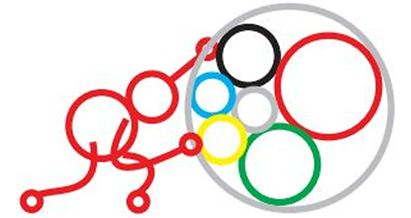
\includegraphics[scale=0.25]{image001.png}}
\end{figure}
\rhead{\LaTeX\ por Axel Aveiga
\\Liceo Cristiano de Guayaquil}
\cfoot{}
%\fancyfoot[R]{\textbf{\LaTeX\ por Axel Aveiga.}}
\begin{center}
\section*{Demostraciones}
\end{center}
\subsection*{1. Teorema de suma de los ángulos de un triángulo.} 
La suma de los ángulos internos de un triángulo es $180^\circ$.
\subsection*{Demostración:}
\begin{center}
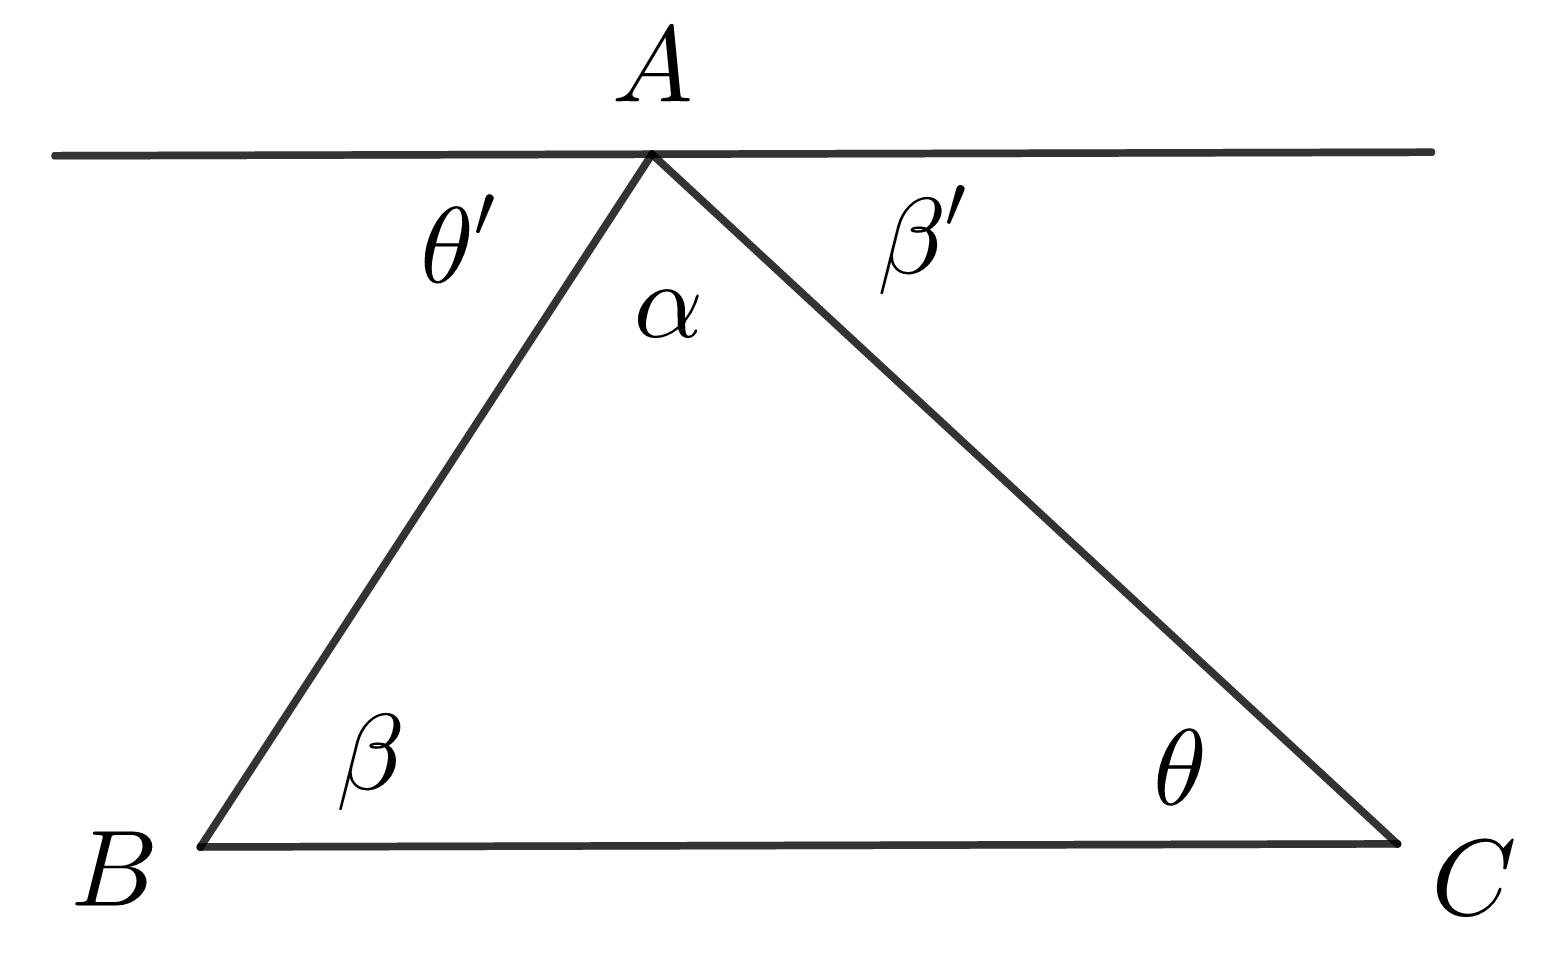
\includegraphics[scale=0.7]{demo1.png}
\end{center}
\begin{tabular}{p{15.9cm} p{1cm}}
Sea un triángulo $ABC$, por el vértice $A$ trazamos una recta paralela al lado $BC$. 
\\Definimos el $\angle A=\alpha, \angle B=\beta$ y $\angle C= \theta$ y definimos respectivamente los  ángulos alternos internos que están en la paralela a $BC$ como $\beta '$ y $\theta '$. & \medskip (1)
\\Por definición y ser ángulo alternos internos, $\beta= \beta '$ y $\theta=\theta '$ &(2)
\\Por (1), los ángulos $\alpha,\beta'$ y $\theta'$ forman un ángulo llano. & (3)
\\Por (2) y (3), $\alpha + \beta+ \theta = \alpha + \beta '+ \theta ' = 180^ \circ$ &(4)
\\Por (4), los  ángulos internos de un triángulo sumas $180^\circ$
\end{tabular}
\subsection*{2.1. Desigualdad del triángulo.}
Para cualquier triángulo tenemos que la suma de las longitudes de dos de sus lados es mayor que la longitud del tercer lado. Es decir, si llamamos $a, b$ y $c$ a las longitudes de los lados del triángulo, tenemos que las siguientes tres desigualdades se cumplen
$$a+b>c, \> a+c>b, \> b+c>a$$
\subsection*{Demostración:}
\begin{center}
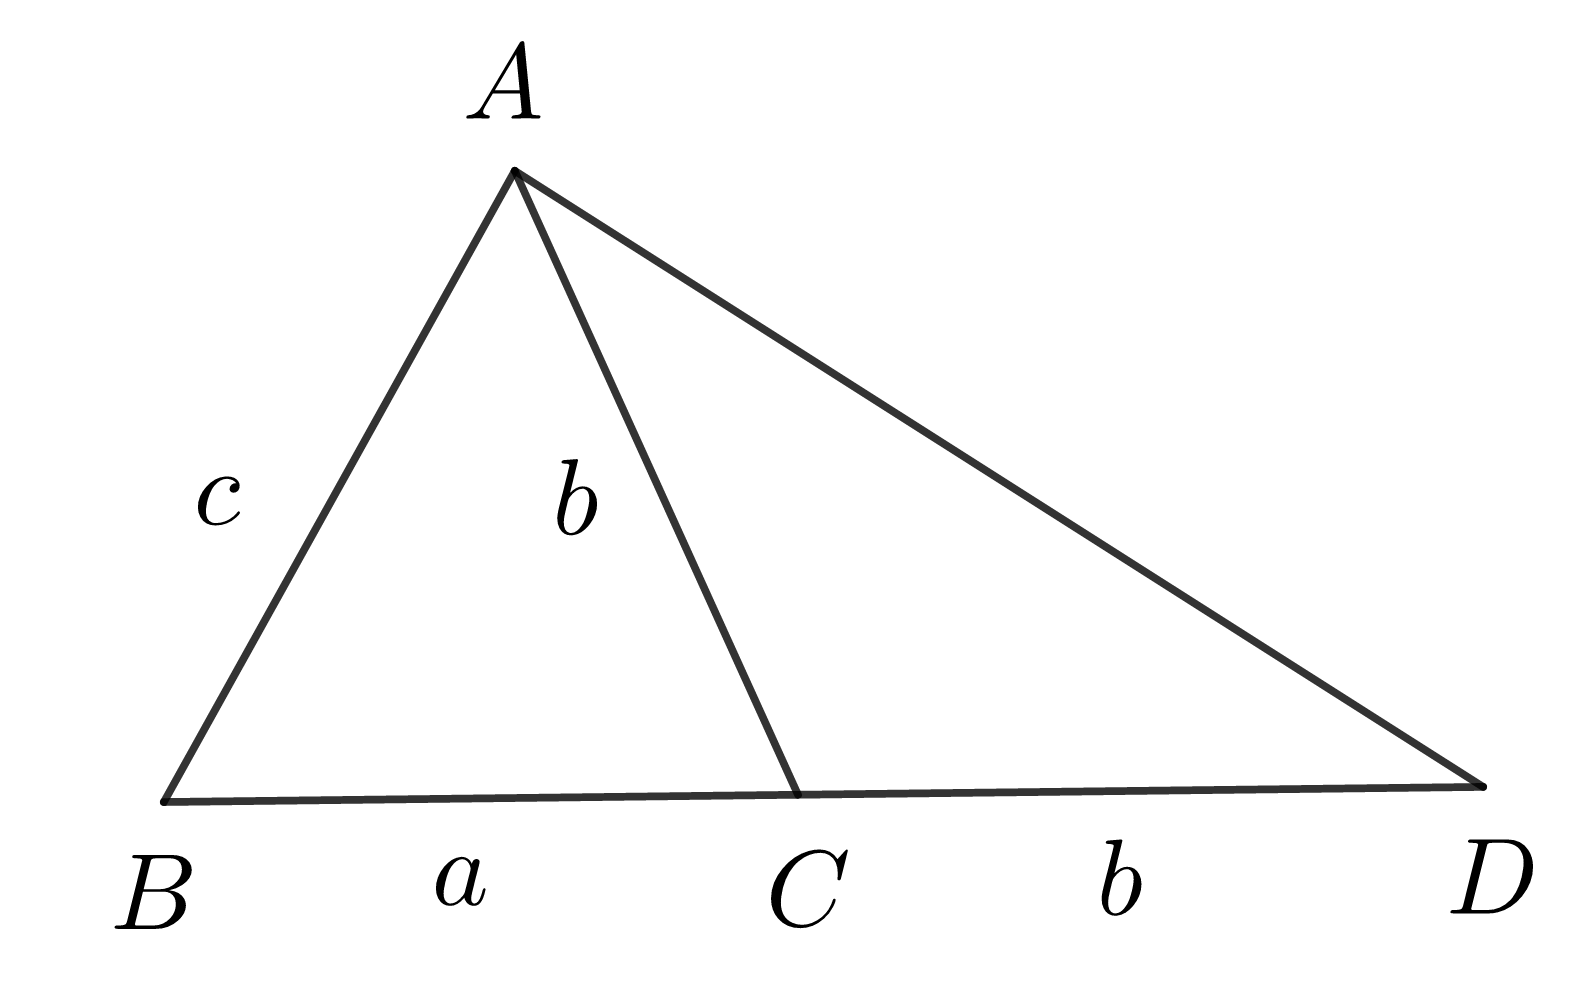
\includegraphics[scale=0.7]{demo2.png} 
\end{center}
\begin{tabular}{p{15.9cm} p{1cm}}\\
Sea $D$ un punto sobre la prolongación del lado $BC$ del triángulo $ABC$, tal que $AC=CD$ & (1)
\\Por (1), $BD=BC+CD=a+b$ & (2)
\\Por (2), el triángulo $ADC$ es isósceles & (3) 
\\Por (3) y $\angle BAD =\angle BAC +\angle CAD$, $\angle BAD > \angle CAD = \angle CDA$ &(4)
\\Se  demostrará lo siguiente, si un triángulo $ABC$ se cumple que $\angle A > \angle B$ entonces $a > b$. &(*)
\\Sea $D$ un punto sobre $AC$ tal que $CD=CB$.
\\Como $\angle A > \angle B$, el punto $D$ no está sobre $\overline{AC}$ & (5)
\\Por (5) y definición de $D$, $CA<CD=BC$ &(6)
\\Por (6), se cumple que $a>b$.
\\Por (4) y (*), $a+b>c$. &
(7)
\\De manera análoga se demuestra que, $a+c>b$ y $b+c>a$.
\end{tabular}
\subsection*{2.2. Teorema.}
Si $a$, $b$ y $c$ son números positivos tales que $a+b>c, a+c>b$ y $c+b>a$, entonces existe un triángulo de lados $a, b$ y $c$.\\
\subsection*{Demostración:}
\begin{center}
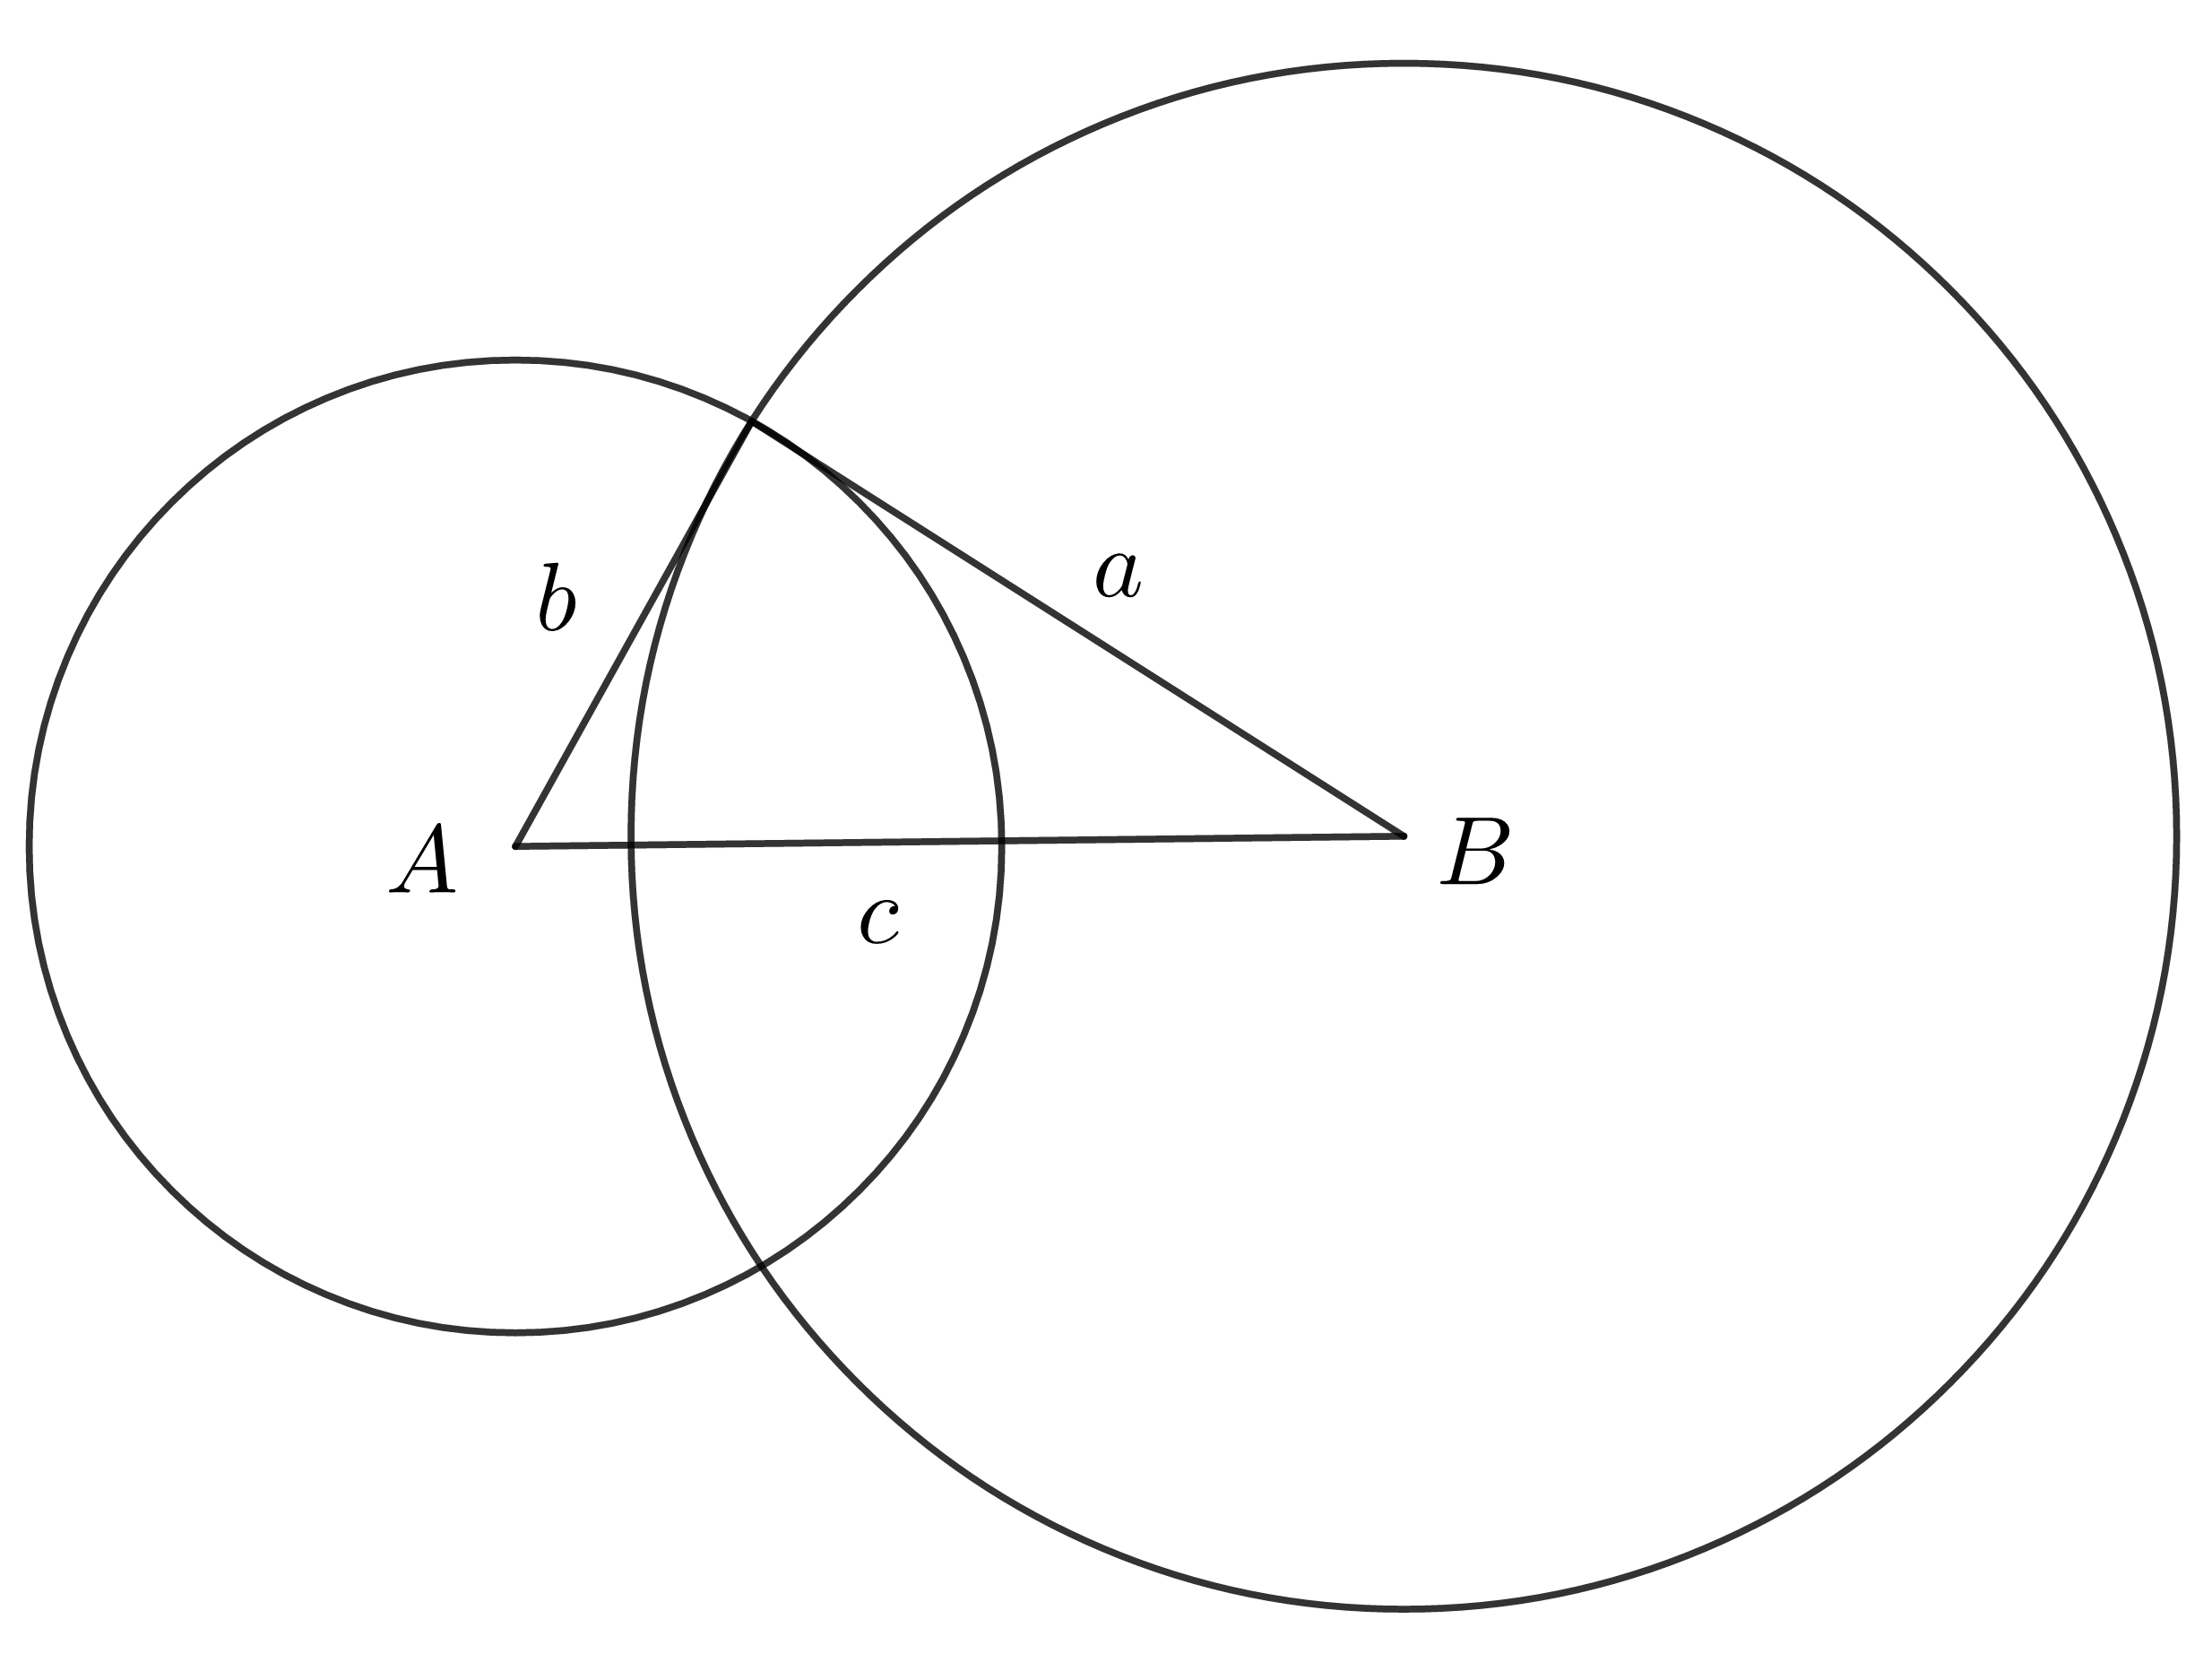
\includegraphics[scale=0.45]{demo3.png} 
\end{center}
\begin{tabular}{p{15.9cm} p{1cm}}
\\Construimos un triángulo con lados iguales a $a, b$ y $c$. 
\\Podemos suponer que $a \leq b \leq c$ y consideramos un segmento $AB$ de longitud $c$.
\\Trazamos ahora dos circunferencias una con centro en $A$ y radio $b$ y otra con centro en $B$ y radio $a$.
\\Como $c<a+b$, las dos circunferencias se intersectan (en caso contrario se tendría que $a+b \leq c)$. Uno de los puntos de intersección sirve como el tercer vértice $C$, del triángulo buscando $ABC$.
\end{tabular}
\subsection*{3.1. Primer teorema de Thales.}
En el triángulo $ABC$, sean $D$ y $E$ puntos de $AB$
y $AC$ respectivamente, tales que $DE$ es paralela a $BC$. Entonces $$\dfrac{AB}{AD}=\dfrac{AC}{AE}$$
\subsection*{Demostración:}
\begin{center}
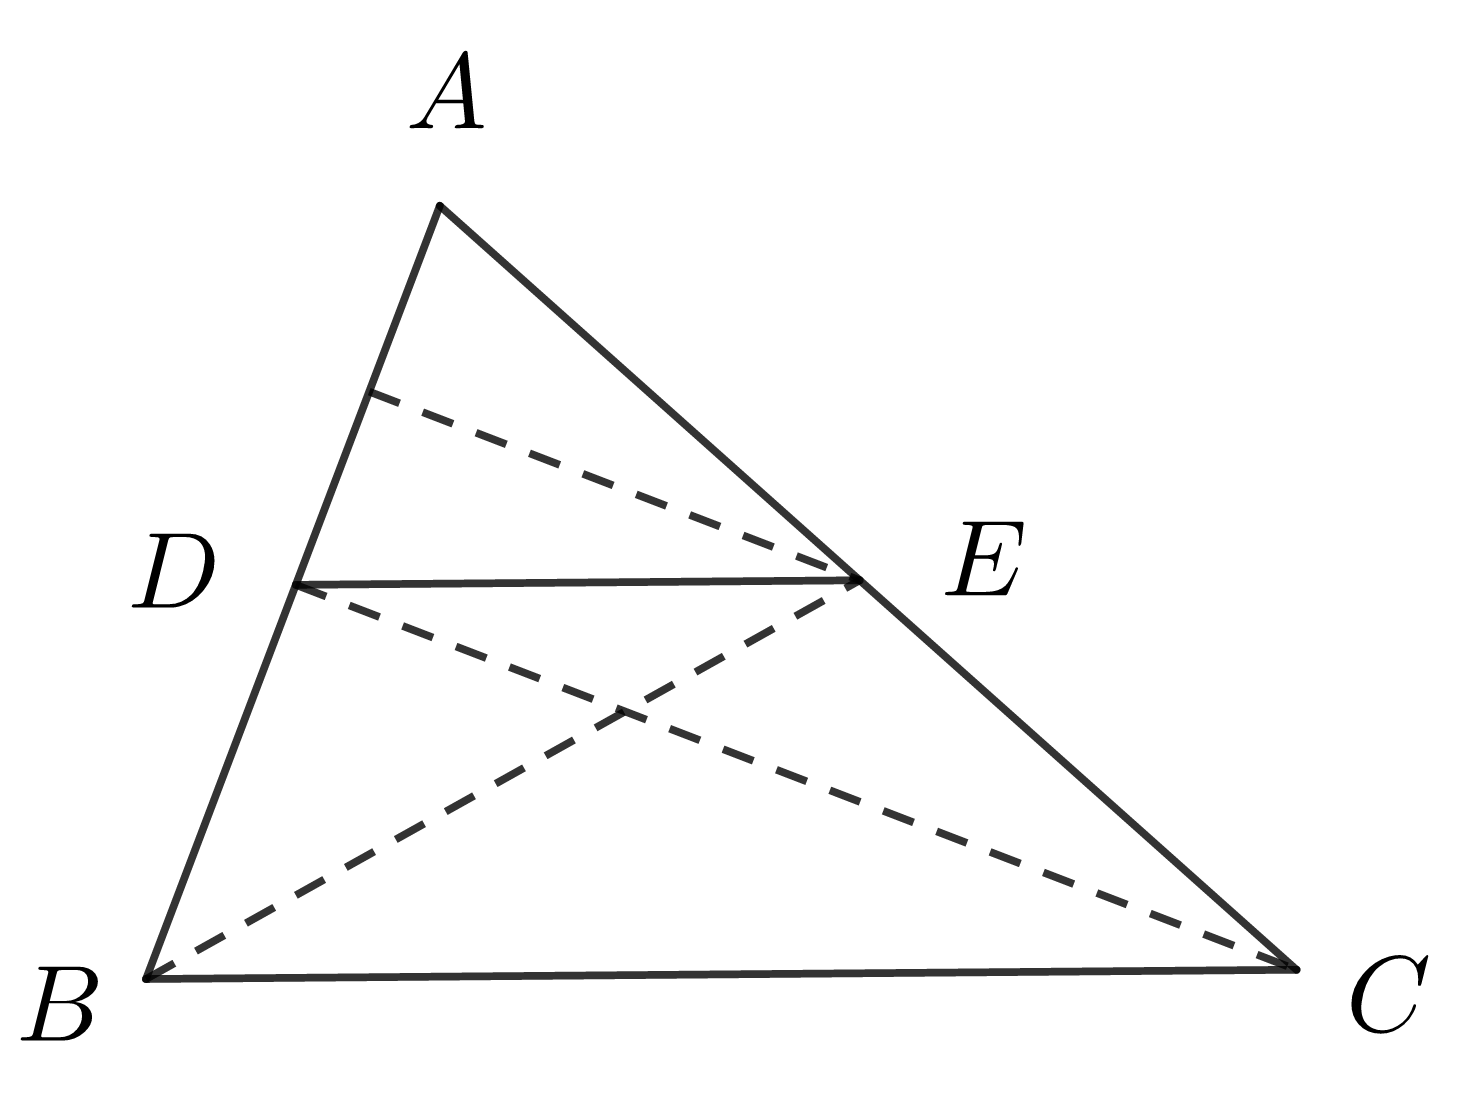
\includegraphics[scale=0.6]{thales 1.png} 
\end{center}
\begin{tabular}{p{15.9cm}p{1cm}}
\\Se considera el triángulo $ABC$ y $DE$ una recta paralela a la base.
\\Por ser $BC$ paralelo a $DE$, los triángulos $ABC$ y $ADE$ tienen alturas paralelas. &(1)
\\Sea la altura $h_1$ que va desde $E$ hacia $AB$ y $h_2$ que va desde $C$ hacia $AB$. &(2)
\\Por (1) y (2), $\dfrac{(ABE)}{(ADE)}=\dfrac{h_1 \cdot AB }{h_1 \cdot AD}=\dfrac{AB}{AD}$ &(3)
\\Análogamente a (3), $\dfrac{AC}{AE}=\dfrac{(ADC)}{(ADE)}$ &(4)
\\Los triángulos $DEB$ y $DEC$ tienen  $DE$ como base común y como $DE$ y $BC$ son paralelos, las respectivas alturas miden lo mismo. &\medskip(5)
\\Por (5), $(DBE)= (DCE)$& (6)
\\Por (6), $(ABE)=(ADE)+(DBE)=(ADE)+ (DCE)= (ADC)$ & (7)
\\Por (3), (4) y (7); tenemos que $\dfrac{AB}{AD}=\dfrac{AC}{AE}$
\end{tabular}
\subsection*{3.1.1. Teorema.}
 Si en el triángulo $ABC$ tenemos puntos $D$ y $E$ sobre los lados $AB$ y $AC$ respectivamente, tales que $$\dfrac{AB}{AD}=\dfrac{AC}{AE}$$
entonces $DE$ es paralela a $BC$.
\subsection*{Demostración:} 
\begin{center}
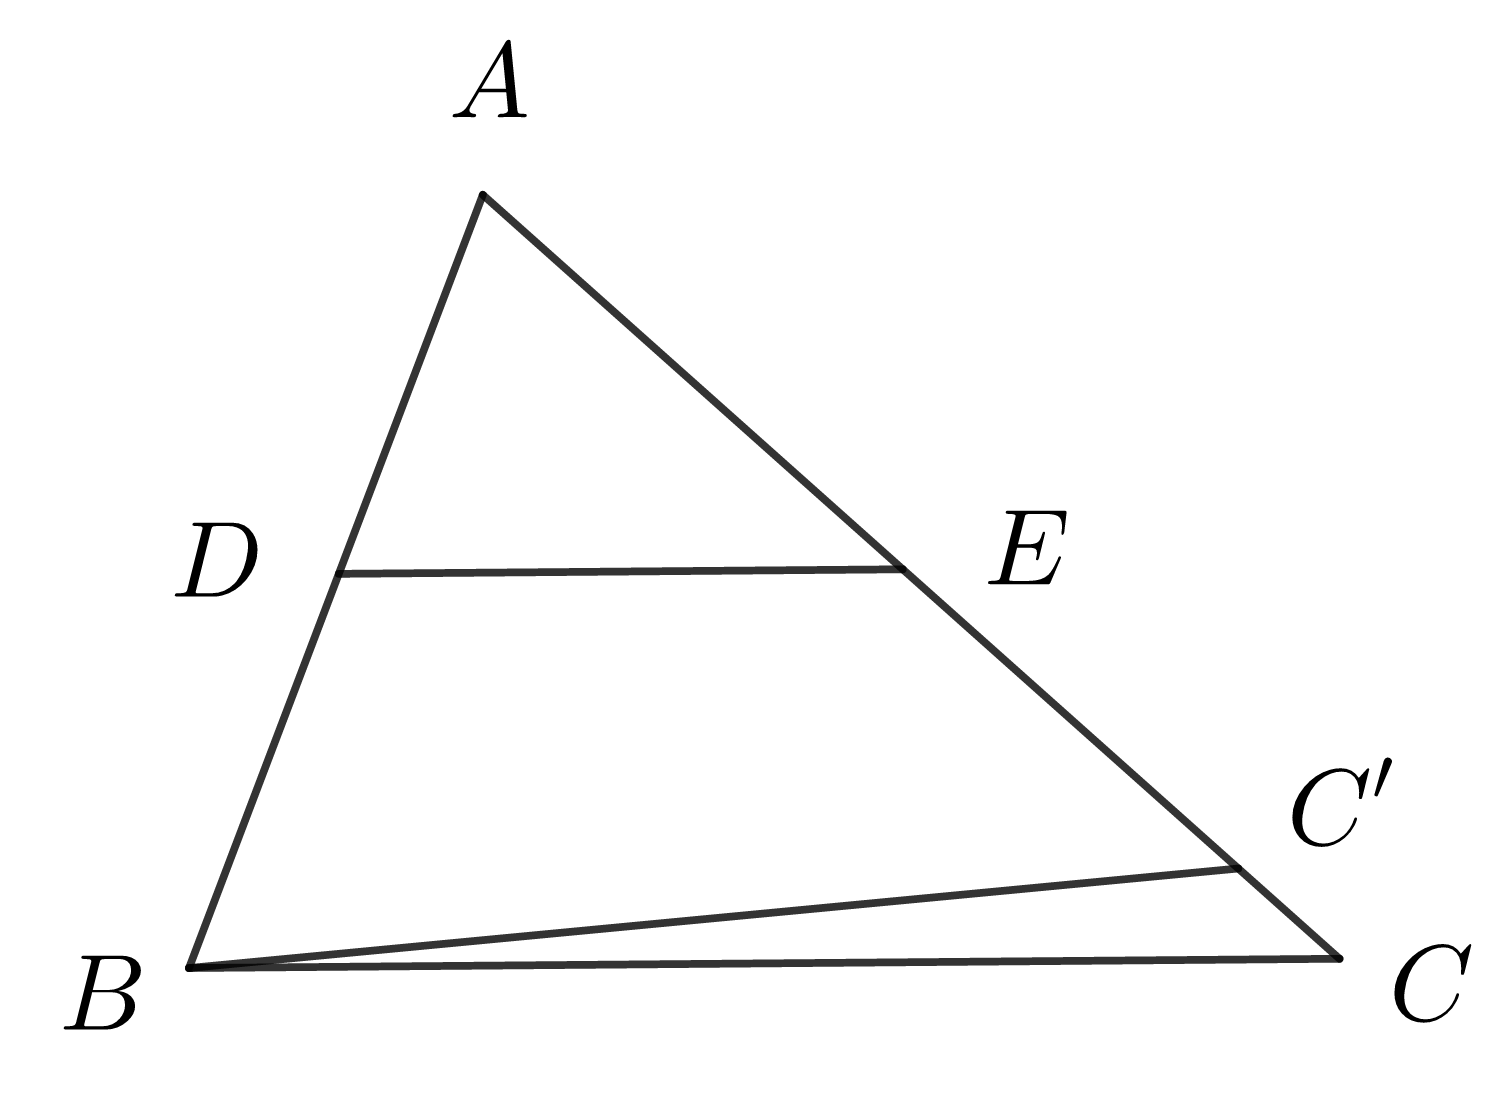
\includegraphics[scale=0.6]{thales1.1.png} 
\end{center}
\begin{tabular}{p{15.9 cm}p{1 cm}}
Supongamos que $DE$ no es paralela a $BC$. Sea $BC'$ la recta que pasa por $B$ paralela a $DE$ y supongamos que intersecta a $AC$ en $C"$.
\\Por el primer teorema de Thales, $\dfrac{AB}{AD}=\dfrac{AC'}{AE}$. & (1)
\\Por hipótesis, $\dfrac{AB}{AD}=\dfrac{AC}{AE}$. & (2) 
\\Por (1) y (2), $\dfrac{AC'}{AE}=\dfrac{AC}{AE}$. &(3)
\\Por (3), $AC'=AC$. & (4) 
\\Por (4), $C'=C$ entonces $DE$ es paralela a $BC$.
\end{tabular}
\subsection*{3.2 Segundo teorema de Thales.}
Consideremos tres rectas y dos rectas transversales a éstas como se muestra en la figura. Tenemos que si $AD, BE$ o $CF$ son paralelas entonces $\dfrac{AB}{BC}=\dfrac{DE}{EF}$, Recíprocamente, si $\dfrac{AB}{BC}=\dfrac{DE}{EF}$ y dos de las rectas $AD, BE$ o $CF$ son paralelas entonces las tres rectas son paralelas.
\begin{center}
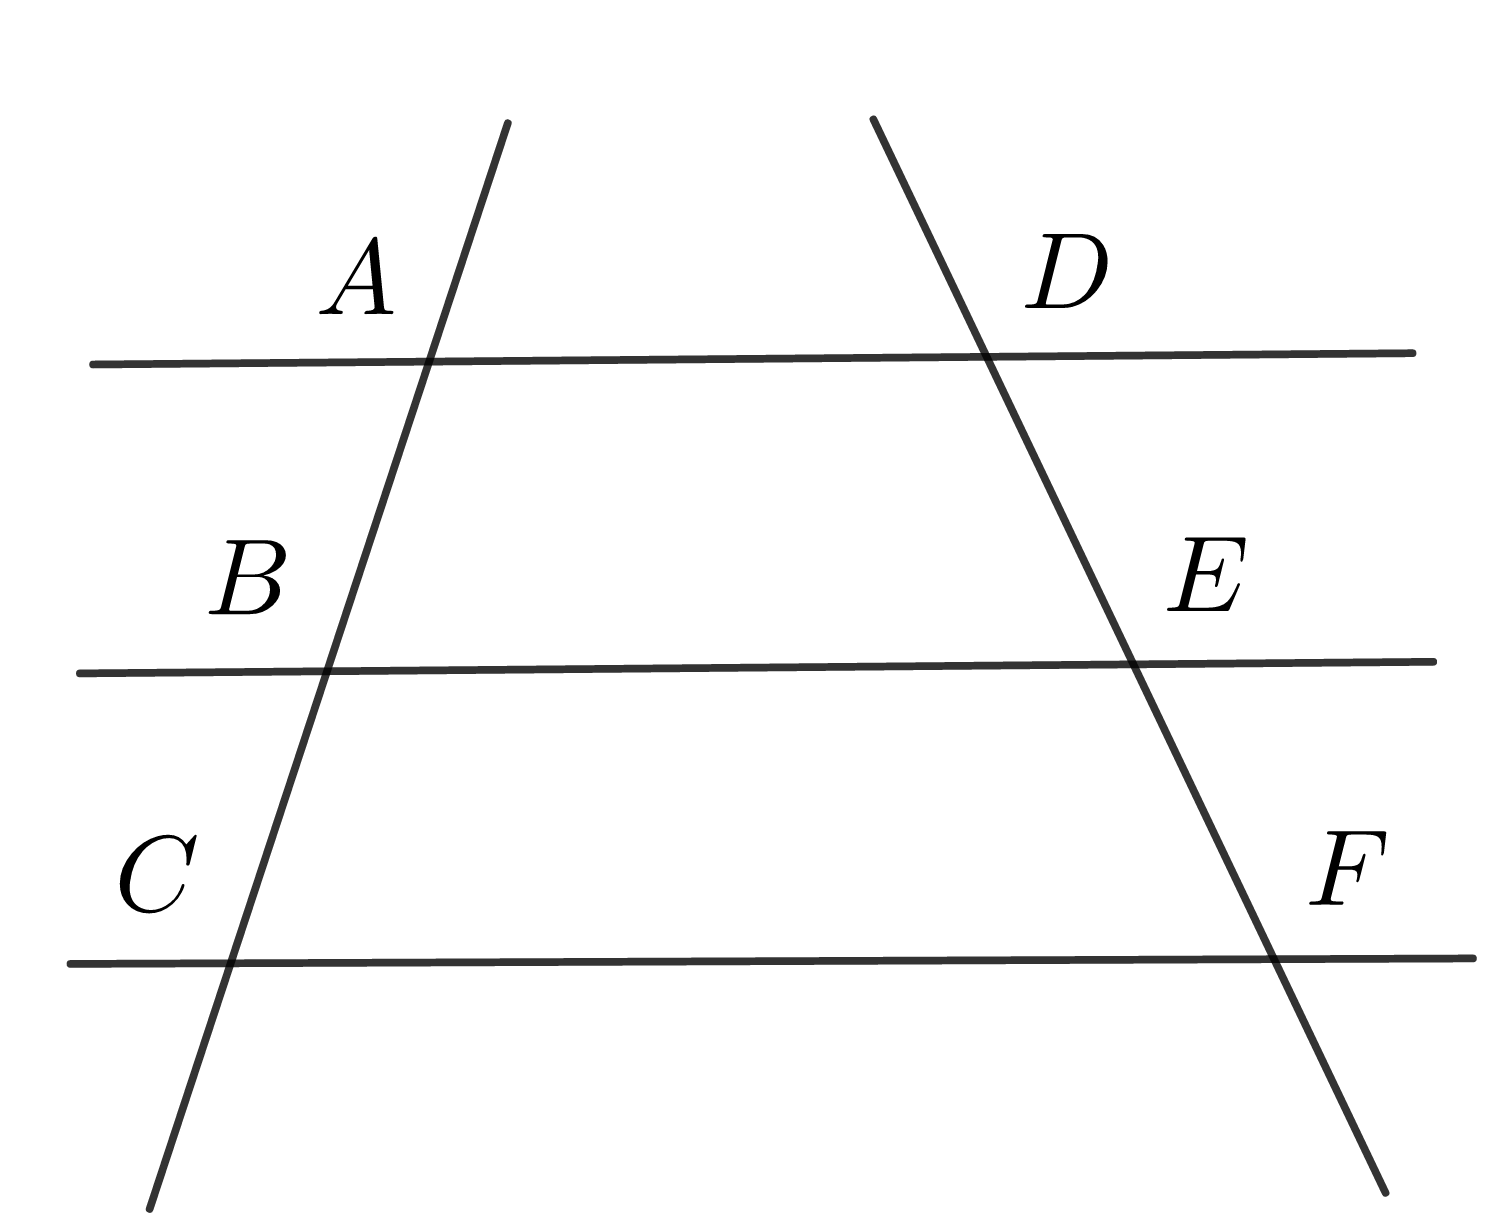
\includegraphics[scale=0.6]{thales.png} 
\end{center}
\subsection*{Demostración:}
\begin{center}
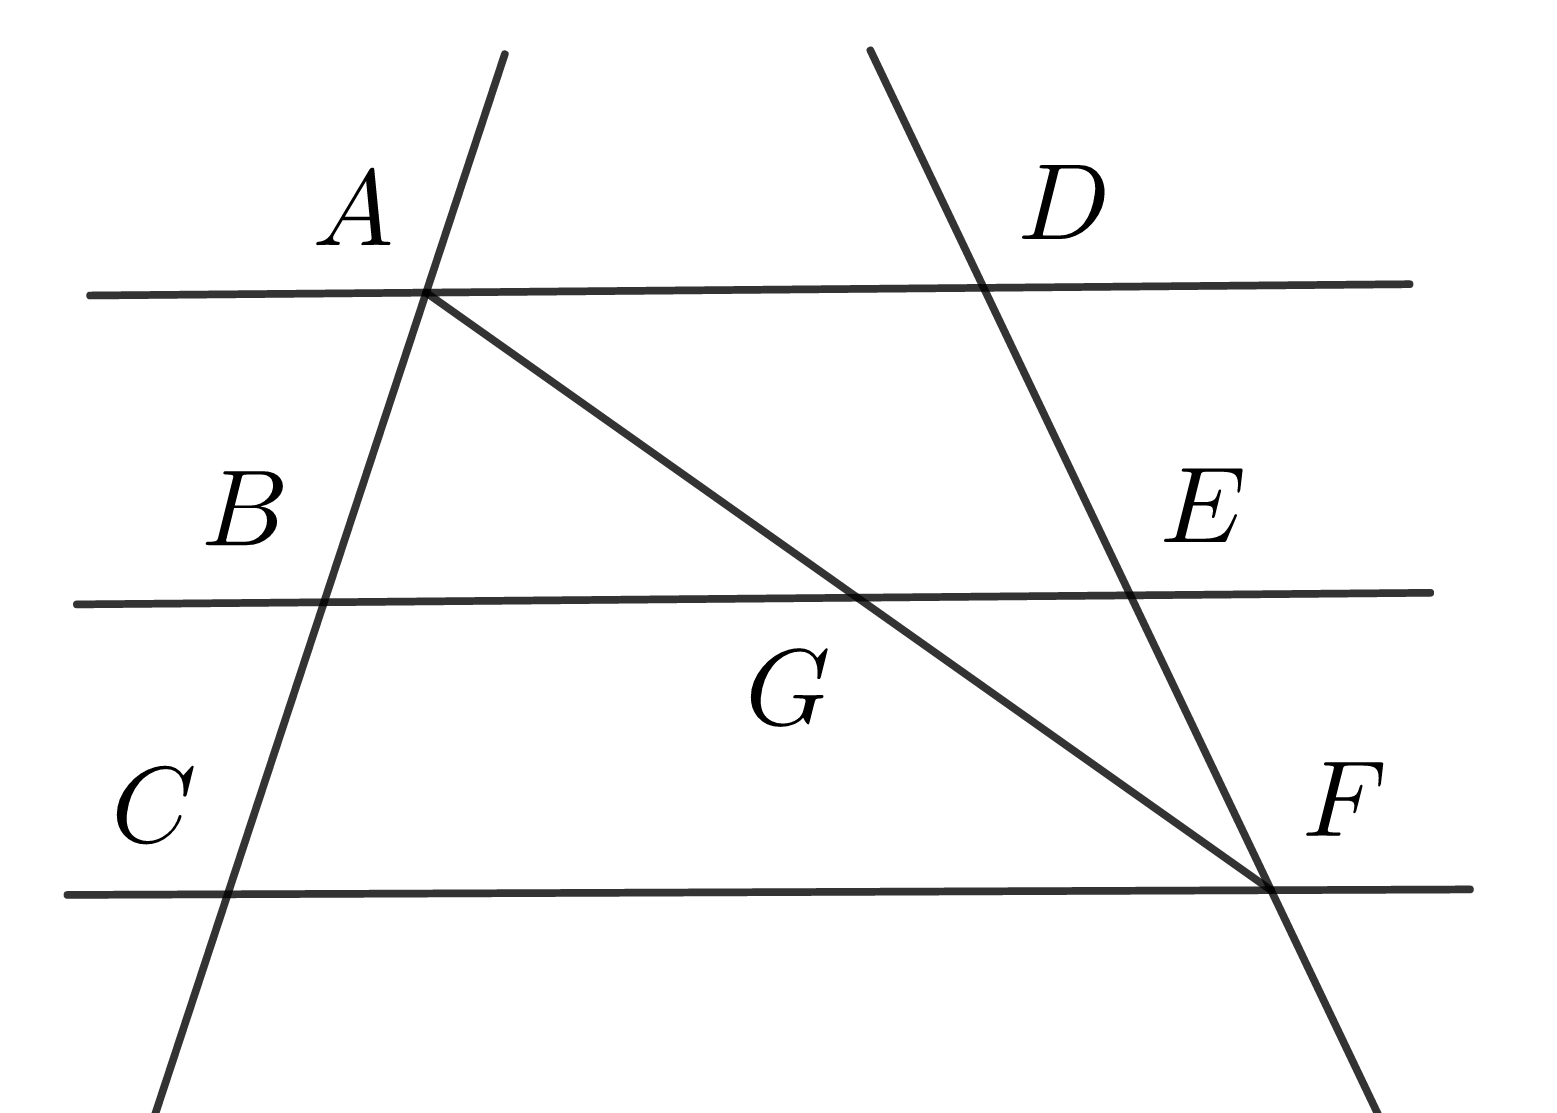
\includegraphics[scale=0.6]{thales2.png} 
\end{center}
\begin{tabular}{p{15.9cm} p{1cm}}
Sea la transversal $AF$ a las tres rectas $AD$, $BE$ y $CF$ y llamamos $G$ al punto de intersección de $AF$ con $BE$.
\\Aplicando el teorema anterior a los triángulos $ACF$ y $FAD$, que las rectas $AD$, $BE$ y $CF$ son paralelas si y sólo si
$$\dfrac{AB}{BC}=\dfrac{AG}{GF} \> \>  y \> \> \dfrac{FG}{GA}=\dfrac{FE}{ED}$$
\\Son paralelas si y sólo si $\dfrac{AB}{BC}=\dfrac{ED}{FE}=\dfrac{DE}{EF}$ & (1)
\\Supongamos que $BE$ y $CF$ son paralelas y que la otra reta $AD$ cumple que $\dfrac{AB}{BC}=\dfrac{DE}{EF}$ &(2)
\\ Por ser $BE$ y $CF$ paralelas, $\dfrac{AB}{BC}=\dfrac{AG}{GF}$&(3)
\\Por ser (2) y (3), $\dfrac{DE}{EF}=\dfrac{AG}{GF}.$ & (4)
\\Por (4) y el primer teorema de Thales, $GE$ y por lo tanto $BE$ es paralelo a $AD$. 
\end{tabular}
\subsection*{4.1. Teorema de semejanza $\angle - \angle - \angle$}
Si dos triángulos tienen sus ángulos correspondientes iguales entonces sus lados correspondiente son proporcionales y los triángulos son semejantes.
\subsection*{Demostración:}
\begin{center}
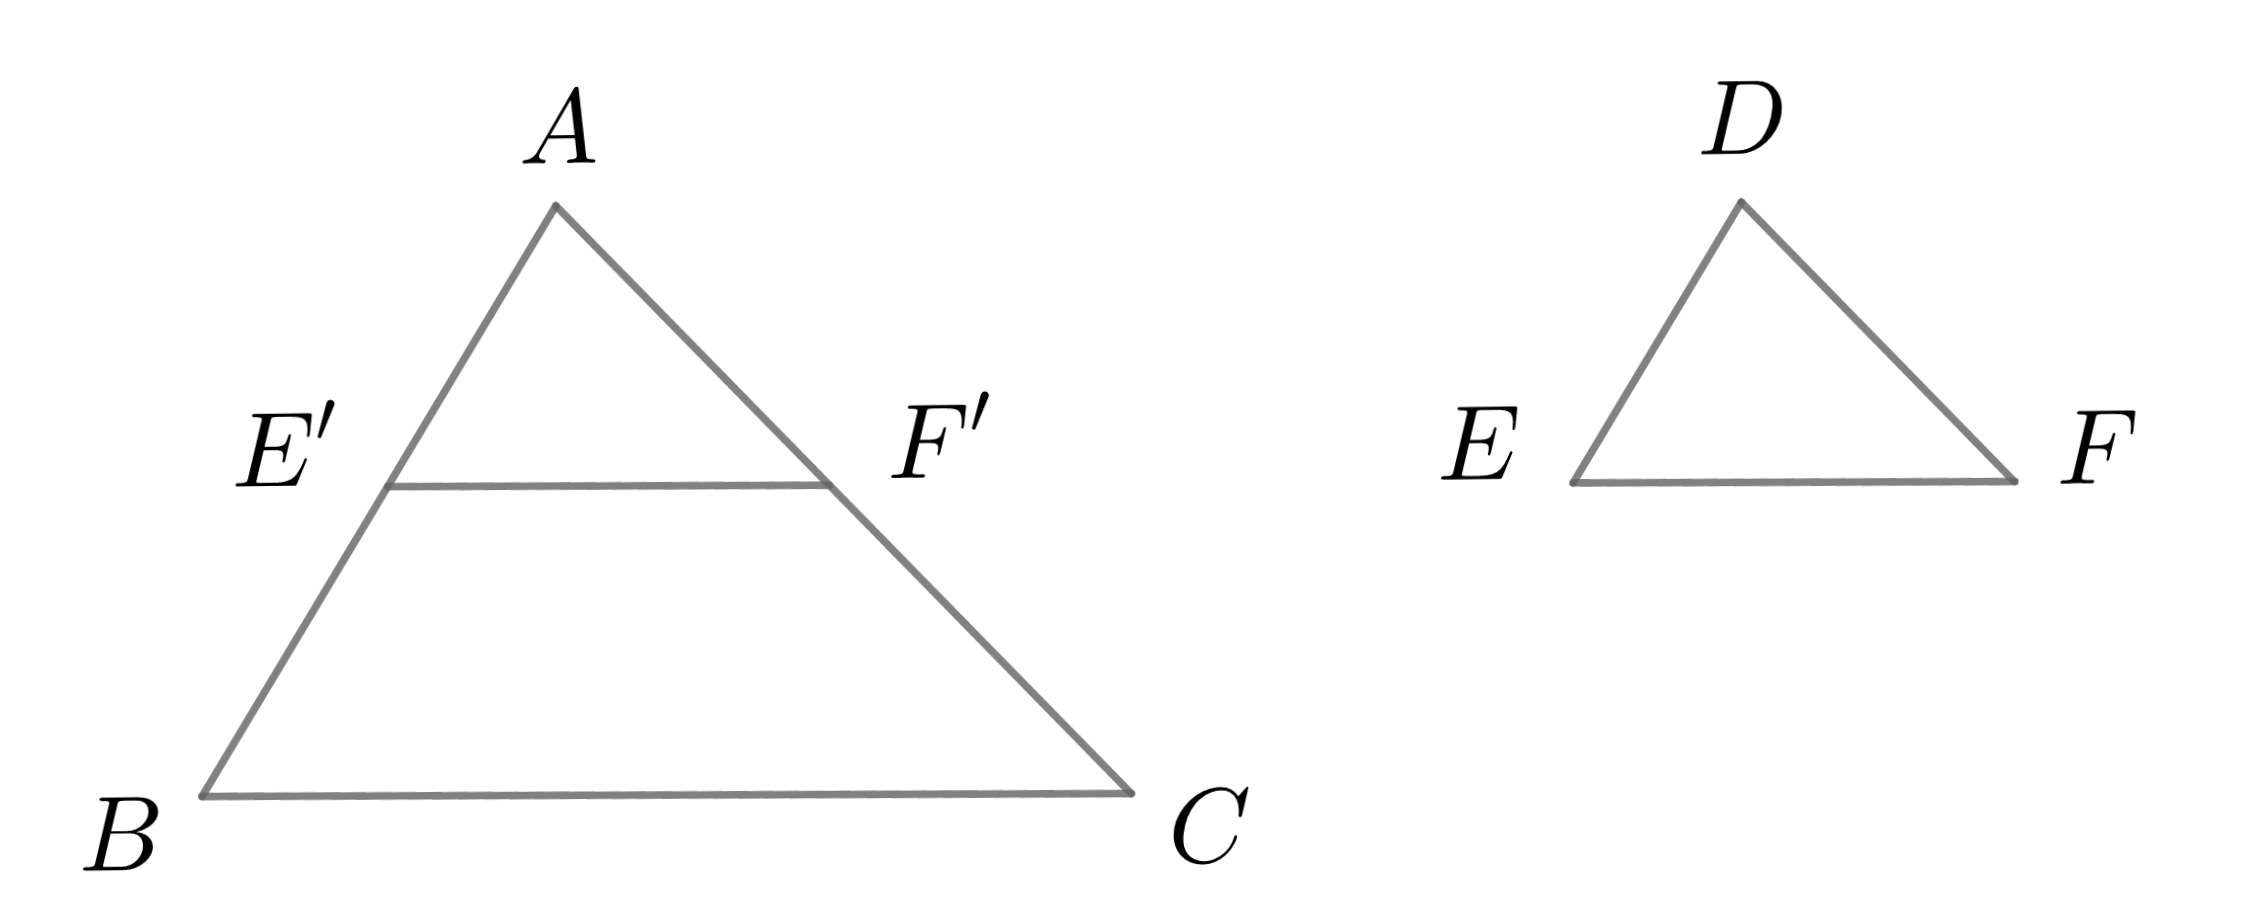
\includegraphics[scale=0.8]{semejanza.png} 
\end{center}
\begin{tabular}{p{15.9 cm} p{1cm}}
Por definición para que dos triángulos sean semejantes se debe cumplir las siguientes condiciones.
\\Todos sus ángulos sean iguales y que $\dfrac{AB}{A'B'}=\dfrac{BC}{B'C'}=\dfrac{CA}{C'A'}.$ 
\\Sean $ABC$ y $DEF$ dos triángulos con ángulos correspondientes iguales, el problema es equivalente a demostrar que $\dfrac{AB}{DE}=\dfrac{CA}{FD}=\dfrac{BC}{EF}.$&\medskip (1)
\\Sean $E'$ y $F'$ dos puntos $AB$ y $AC$ respectivamente, tales que $AE'= DE$ y $AF' = DF$. &(2)
\\Por criterio de congruencia $L-A-L$, tenemos que los triángulos $AEF$ y $DEF$ son congruentes.&(3)
\\Por (3), $\angle AE'F' = \angle DEF $ & (4)
\\Por hipótesis y (4) $\angle AE'F'=\angle ABC$ & (5)
\\Por (5), son $E'F'$ y $BC$ paralelas. & (6)
\\Por (6) y el primer teorema de Thales, $\dfrac{AB}{AE'}=\dfrac{AC}{AF'}$ & (7)
\\Por (2) y (6), $\dfrac{AB}{DE}=\dfrac{AC}{DF}$
\\De manera análoga se demuestra que $\dfrac{AB}{DE}=\dfrac{CA}{FD}=\dfrac{BC}{EF}.$ & (8)
\\Por (1) y (8), se cumplen el teorema de semejanzas $A-A-A$.
\end{tabular}
\subsection*{4.2 Teorema de semejanza $L- \angle -L$.}
Si dos triángulos tienen dos lados correspondientes proporcionales y el ángulo comprendido entre éstos es igual, entonces son semejantes.
\subsection*{Demostración:} 
\begin{center}
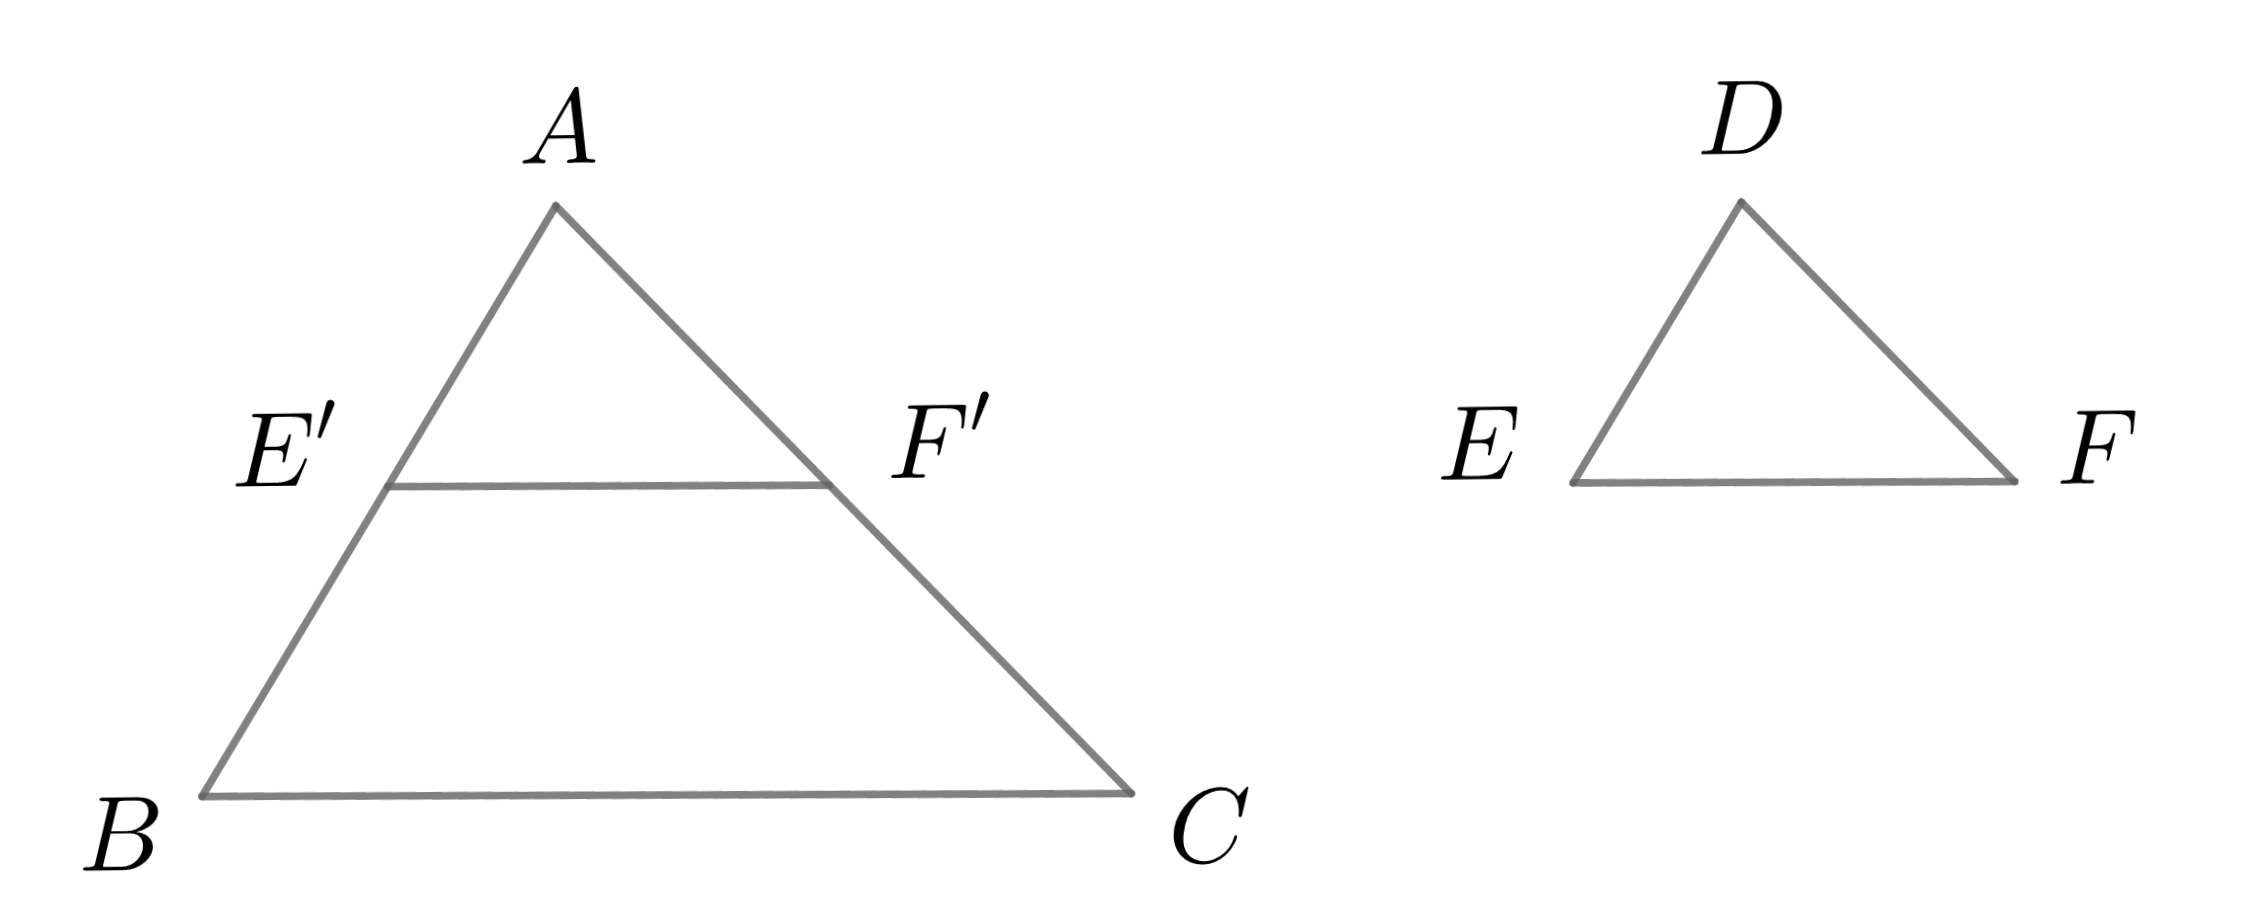
\includegraphics[scale=0.8]{semejanza.png} 
\end{center}
\begin{tabular}{p{15.9cm} p{1cm}}
Por hipótesis y sin perdida de generalidad se considera dos triángulos $ABC$ y $DEF$ tales que $\dfrac{AB}{DE}=\dfrac{AC}{DF}$ y $\angle BAC=\angle EDF$
\\Sean $E'$ y $F'$ los puntos sobre el lado $AB$ y $AC$ tales que $AE'=DE$ y $AF'=DF$& (1)
\\Por el criterio de congruencia $L-A-L$, tenemos que los triángulos $AE'F'$ y $DEF$ son congruentes. &\medskip(2)
\\Por (2), $\dfrac{AB}{AE'}=\dfrac{AC}{AF'}$ &(3)
\\Por el teorema fundamental de la proporcionalidad (Teorema 3.1.1), $EF$ es paralelo a $BC$. &(4) 
\\Por (4), los ángulos $\angle ABC$ y $\angle AEF$ son iguales. &(5)
\\Por hipótesis y (5), $\angle BAC= \angle EAF$&(6)
\\Por (6) y el teorema de semejanza $A-A-A$, los triángulos $ABC$ y $AE'F'$ son semejantes&(7)
\\Por (7), los triángulos $ABC$ y $DEF$ son semejantes. &(8)
\\Por(8), se cumple el teorema de semejanza de $L-A-L$.
\end{tabular}
\subsection*{4.3 Teorema de semejanza $L-L-L$.}
Si dos triángulos tienen sus lados correspondientes proporcionales entonces los triángulos son semejantes.\\
\begin{tabular}{p{15.9cm}p{1cm}}
\subsection*{Demostración:}
\begin{center}
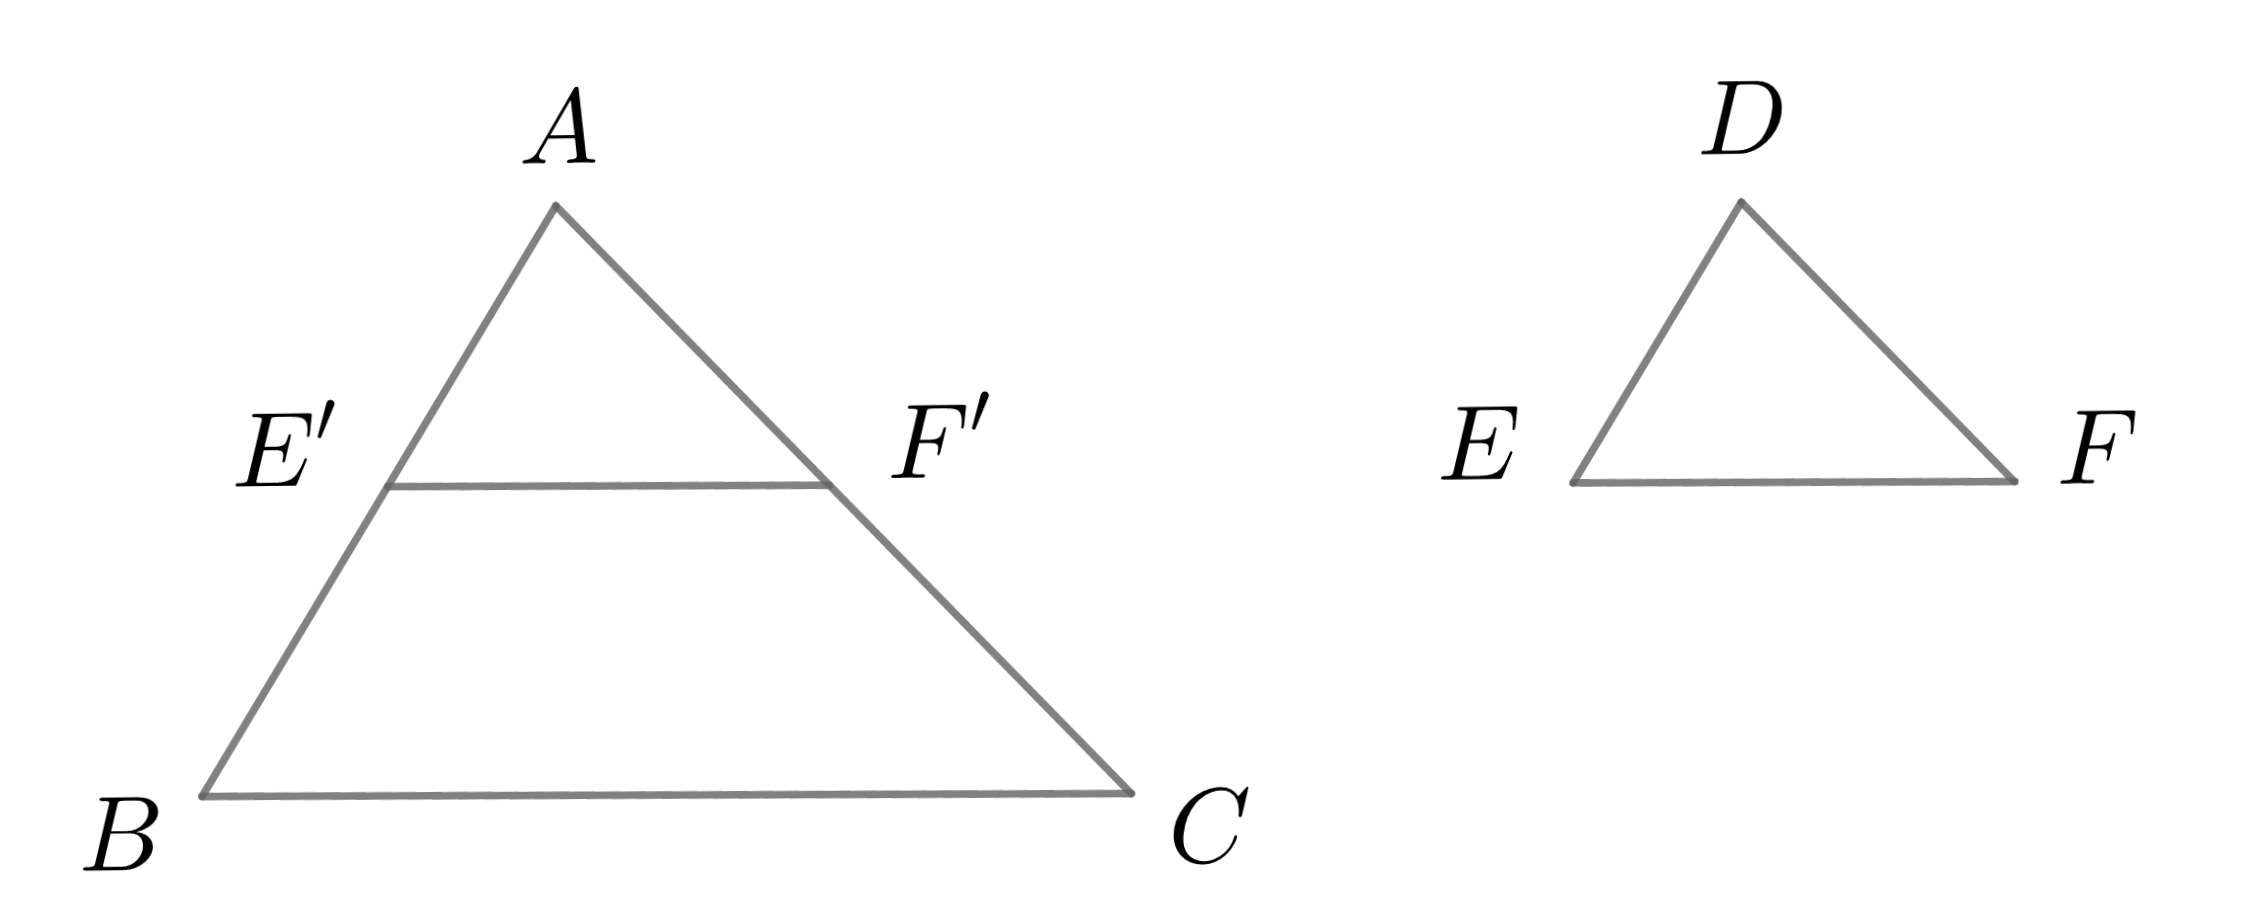
\includegraphics[scale=0.75]{semejanza.png} 
\end{center} 
\\Por hipótesis sean $ABC$ y $DEF$ dos triángulos que cumplen: $\dfrac{AB}{DE}=\dfrac{BC}{EF}=\dfrac{AC}{DF}$ & (1)
\\Sean $E'$ y $F'$ los puntos en $AB$ y $AC$ respectivamente, tales que $DE = AE'$ y $DF= AF'$ &(2)
\\Sustituyendo (2) en (1), $\dfrac{AB}{AE'}=\dfrac{AC}{AF'}$&(3)
\\ Por definición los triángulos $ABC$ y $AEF$ comparten el ángulo en $A$ &(4)
\\Por (1), (4) y el teorema de semejanza $L-A-L$, los triángulos $ABC$ y $AE'F'$ son semejantes. &(5)
\\Por definición de semejanza, $\dfrac{E'F'}{BC}=\dfrac{AE'}{AB}$ &(6)
\\Por (2) y (6), $E'F'=BC\dfrac{DE}{AB}$. & (7)
\\Por (1) y (7), $EF=E'F'$ & (8)
\\Por hipótesis (8) y el criterio de congruencia $L-L-L$, los triángulos $AE'F'$ y $DEF$ son congruentes &\medskip(9)
\\Por (9), los triángulos $ABC$ y $DEF$ son semejantes
\end{tabular}
\subsection*{5.1 Teorema de Pitágoras.}
En un triángulo rectángulo el cuadrado de la hipotenusa es igual a la suma de los cuadrados de los catetos.
\\
\begin{tabular}{p{15.9 cm} p{1cm}}
\subsection*{Demostración:}
\begin{center}
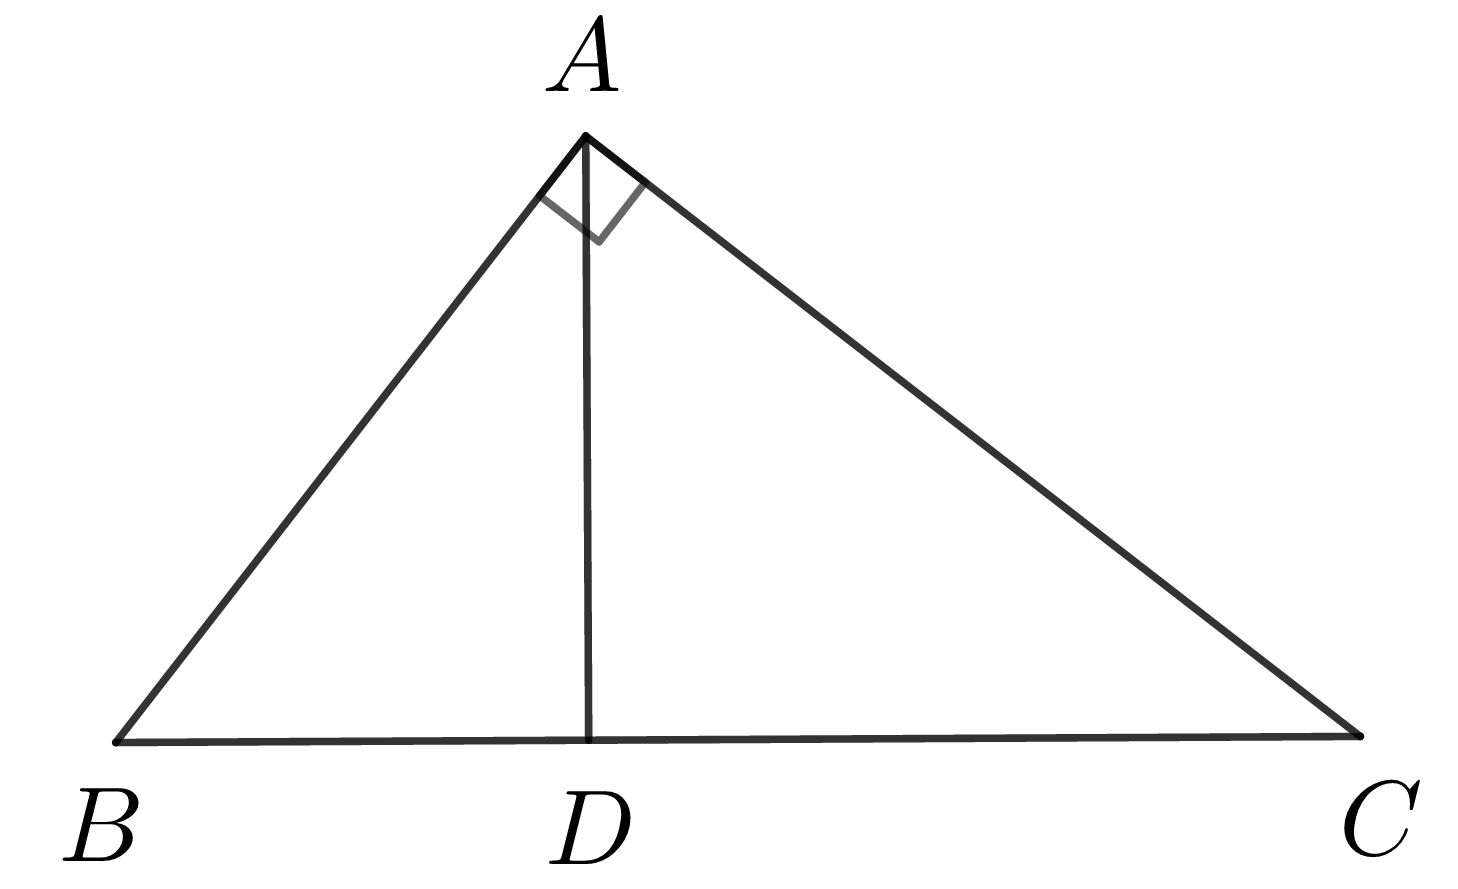
\includegraphics[scale=0.8]{pitagoras.png} 
\end{center}
Sea $ABC$ un triángulo rectángulo con ángulo recto en el vértice $A$ y sea $AD$ altura sobre la hipotenusa $BC$.
\\Por hipótesis y por el teorema de semejanzas de triángulos L-L-L, $ABC$ es semejante a $DBA$. &(1)
\\Análogo a (1), los rectángulos $ABC$ y $DAC$ & (2)
\\Por (1), $\dfrac{AB}{DB}=\dfrac{CB}{AB}$ & (3)
\\Por (3), $AB^2=DB \cdot CB$ &(4)
\\Por (2),  $\dfrac{CA}{CD}=\dfrac{CB}{CA}$ &(5)
\\Por (5), $CA^2=CD.CB$ &(6)
\\AL sumar (4) y (6), tenemos que $AB^2+CA^2=DB\cdot CB + CD\cdot CB$ & (7)
\\Por hipótesis, $DB\cdot CB + CD\cdot CB=(CD +DB)\cdot CB=CB^2$ &(8)
\\Por (7) y (8), $AB^2 + CA^2=CB^2$
\end{tabular}
\subsection*{5.2 Teorema recíproco del Pitágoras.}
Si un triángulo el cuadrado de un lado es igual a la suma de los cuadrados de los otros dos lados, el triángulo es rectángulo.
\begin{center}
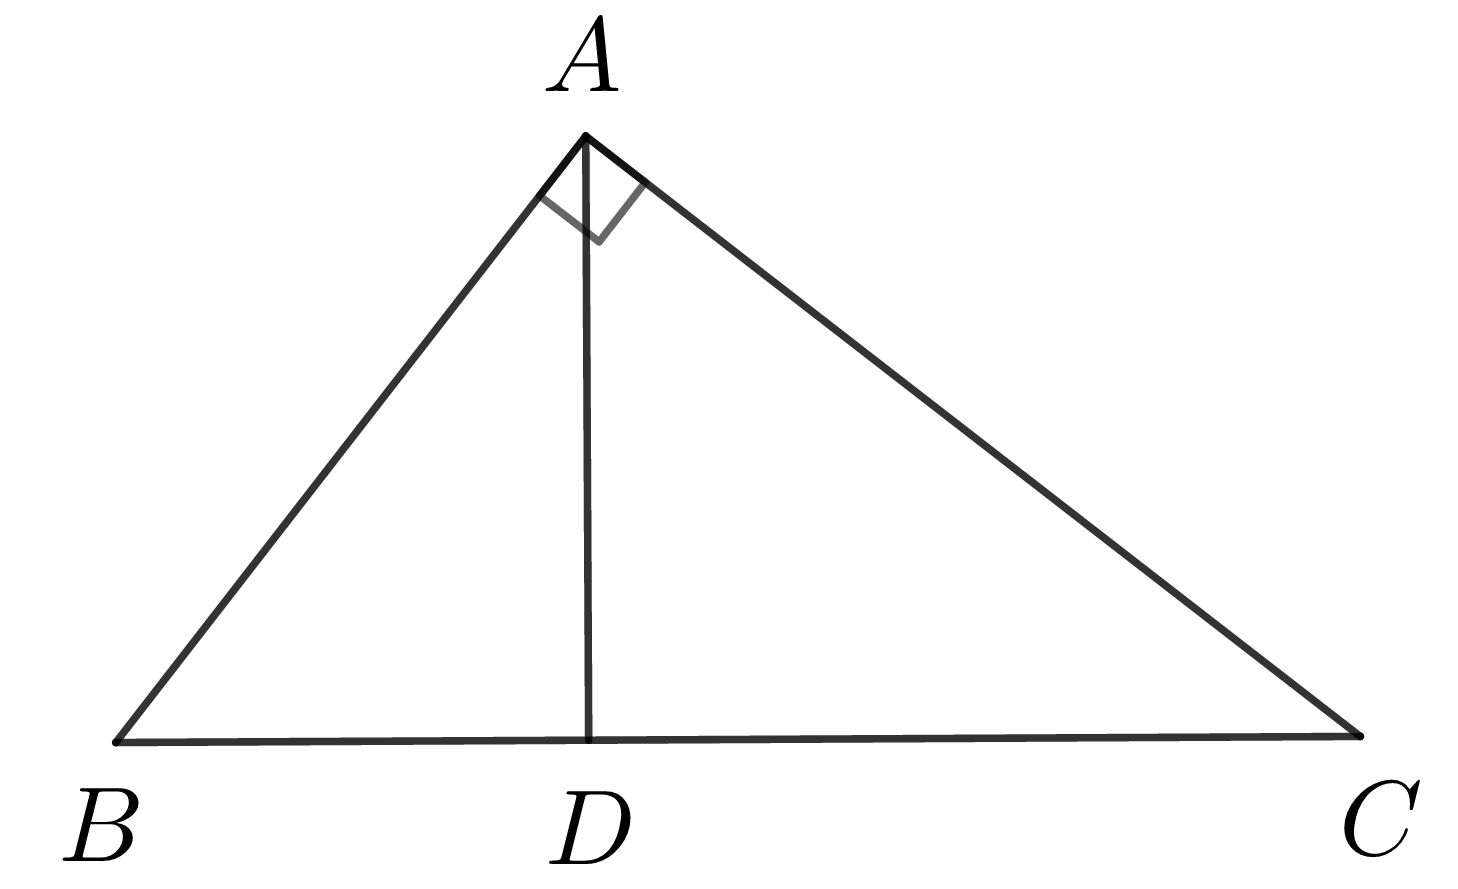
\includegraphics[scale=0.8]{pitagoras.png} 
\end{center}
\subsection*{Demostración:}
\begin{tabular}{p{15.9cm}p{1cm}}
Supongamos que $ABC$ es un triángulo con $BC^2=AB^2+CA^2$. &(1)
\\Por (1), $BC>AB$ y $BC> AC$. &(2)
\\Por(2), los ángulos en $B$ y $C$ son menores a $90^\circ$. 
\\Sea $D$ el pie de la perpendicular de $A$ sobre $BC$.
\\Por ser los triángulos $ABD$ y $ADC$ rectángulos con ángulo recto en $D$ y el teorema de Pitágoras, $AB^2=BD^2+AD^2$ y $CA^2=AD^2+DC^2$. & \medskip(3)
\\Por (3), $2AD^2+ BD^2+DC^2=AB^2+CA^2=BC^2=(BD+DC)^2=BD^2+2BD \cdot DC + DC^2$. &(4) 
\\Por (4), $AD^2 = BD\cdot DC$ &(5)
\\\textbf{Lema:} Sea $ABC$ un triángulo, con ángulos en $B$ y $C$ menores a $90^\cdot$ y sea $D$ el pie de la altura de $A$ sobre $BC$. Si $AD^2=BD\cdot DC$ entonces $ABC$ es triángulo rectángulo.& \medskip (6)
\\Trazamos la perpendicular a $AB$ que pasa por $A$, ésta corta a la recta $BC$ en un punto $C'$ (si no fuera el caso, entonces de tal recta es paralela a $BC$ y resulta entonces que $B=D$, por lo que $AD^2=BD \cdot DC$ sería falso).
\\Por hipótesis, $ABC'$ es un triángulo rectángulo con ángulo recto en $A$.& (7)
\\Por el teorema  de semejanza de triángulo, $\dfrac{AD}{CD'}=\dfrac{BD}{AD}$ & (8)
\\Por (8), $AD^2= BD\cdot DC'$. &(9)
\\Por hipótesis y análogo a (9),$AD^2=BD\cdot DC$.& (10)
\\Por (9) y (10), $DC'=DC$ &(11) 
\\Por (11), $C=C'$. & (12) 
\\Por (12), $ABC$ es triángulo rectángulo y se cumple el lema.
\\Por (5) y (6), se cumple el teorema.
\end{tabular}
\\\\\textbf{Nota:} La condición de que el triángulo no tenga ángulos obtusos en $B$ y $C$, obliga a que $C'$ y $C$ queden del mismo lado con respecto a $D$, entonces $D$ se encuentra entre $B$ y $C$.
\subsection*{6. Teorema.}
Las medianas de un triángulo son concurrentes.
\subsection*{Demostración:}
\begin{center}
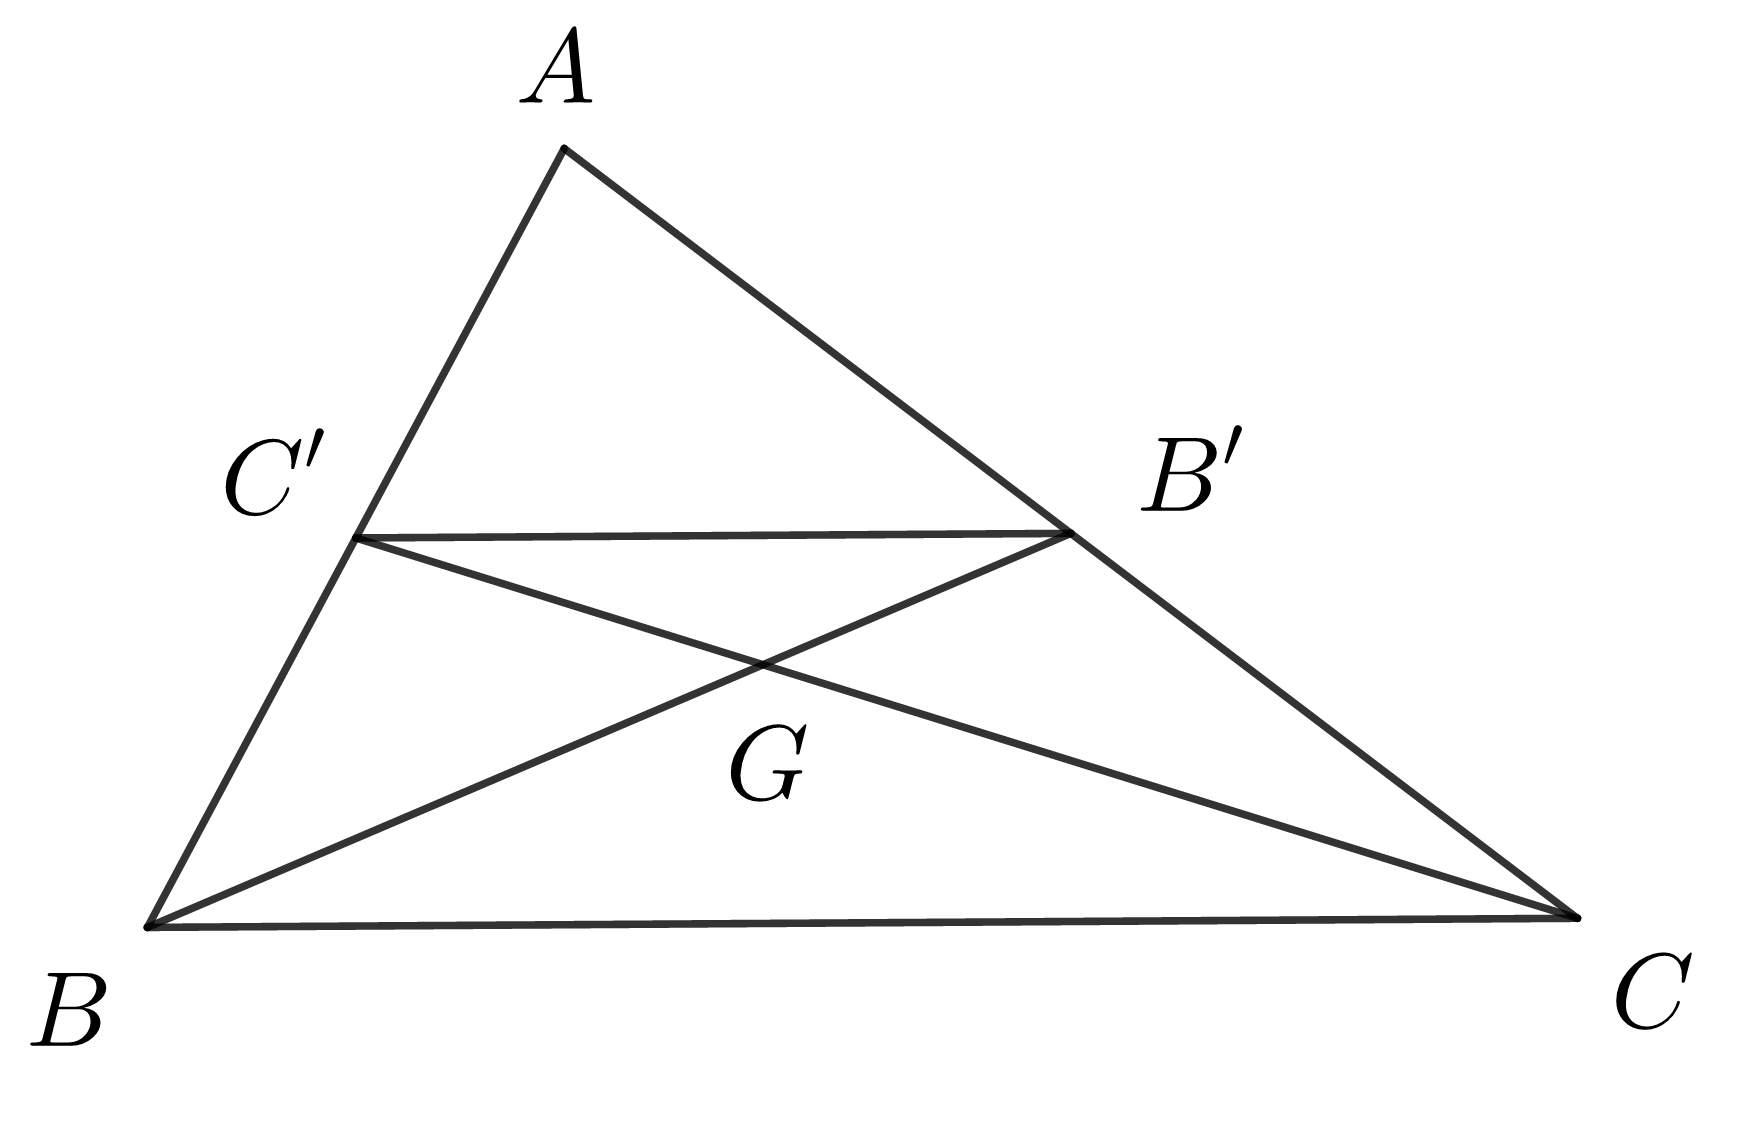
\includegraphics[scale=0.8]{medianas.png} 
\end{center}
\begin{tabular}{p{15.9 cm} p{1cm}}
Sean $ABC$ el triángulo y $A', B', C'$ los puntos medios de $BC, CA$ y $AB$, respectivamente. Sea $G$ el punto de intersección de las medianas $BB'$ y $CC'$. 
\\Por hipótesis y el teorema de Thales, $B'C'$ es paralelo a $BC$. &(1)
\\Por (1) y semejanzas de triángulo, los lados de los triángulos $GBC$ y $GB'C'$ son paralelos. &(2)
\\Por (2), los triángulos son semejantes y en razón de semejanza $2:1.$ &(3)
\\Por (3), las medianas $BB'$  y $CC'$ se cortan en el único punto $G$ que divide a la mediana en razón $2:1$. &\medskip(4)
\\Por (4), $G$ es el único punto sobre $BB'$ con $\dfrac{BG}{GB'}=\dfrac{2}{1}$ y el único sobre $CC'$ con $\dfrac{CG}{GC'}=\dfrac{2}{1}$. &(5)
\\Análogo a (5) se demuestra que la otra mediana $AA'$ se intersecta con $BB'$. &(6)
\\Por (5) y (6), las tres medianas se concurren en $G$.
\end{tabular}
\subsection*{7. Teorema.}
Las bisectrices internas de un triángulo son concurrentes.
\\
\begin{tabular}{p{15.9cm}p{1cm}}
\subsection*{Demostración:}
\begin{center}
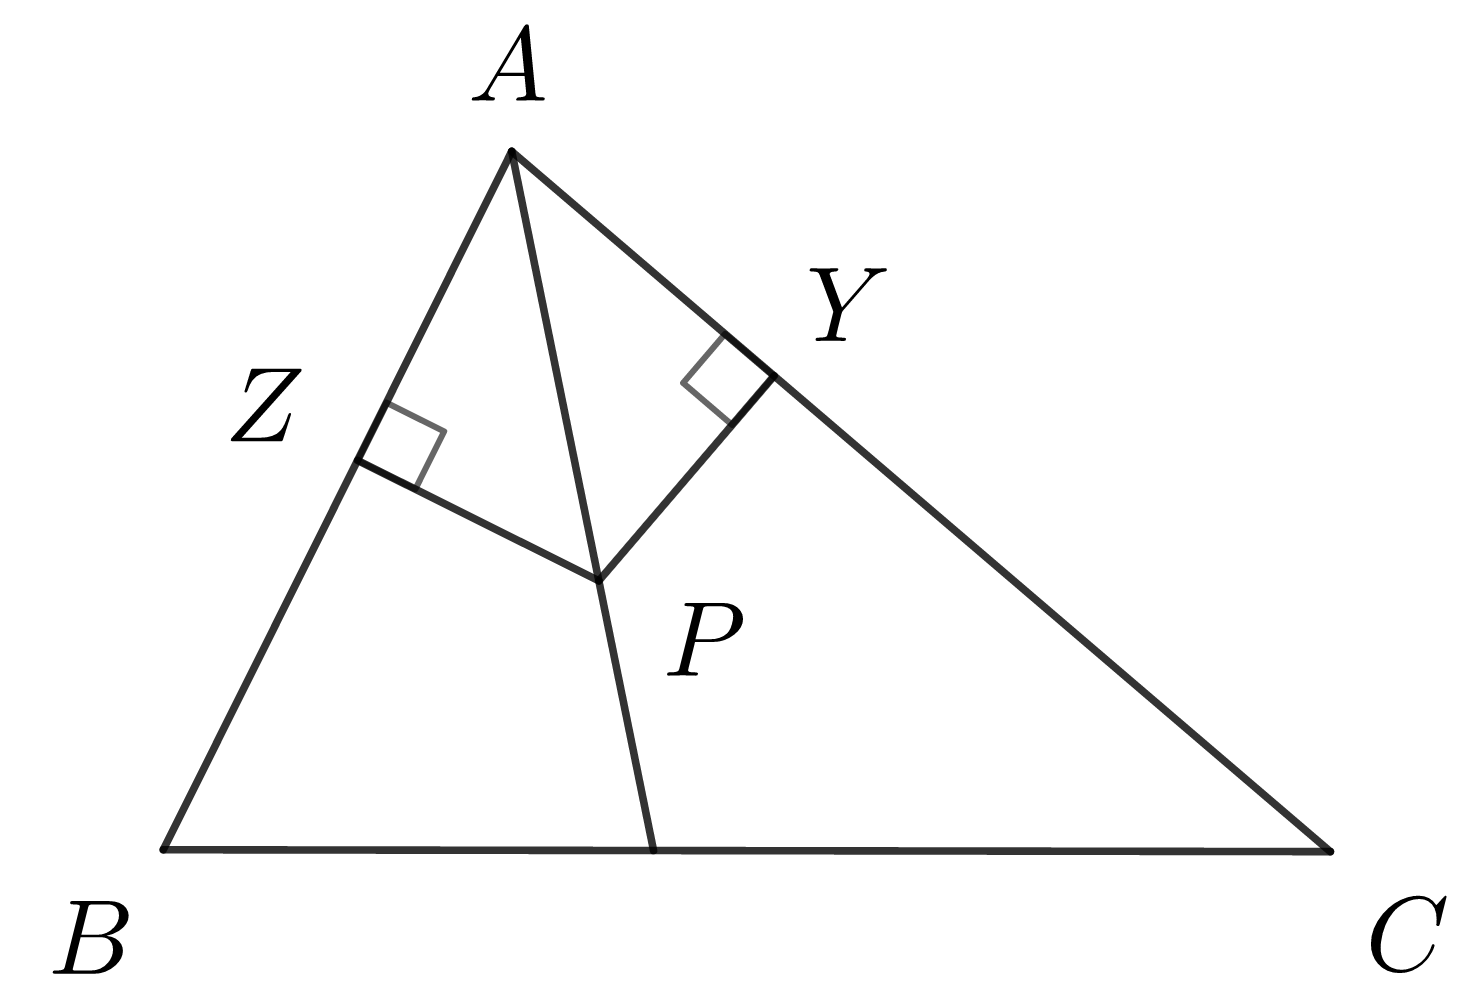
\includegraphics[scale=0.5]{bisectriz.png} 
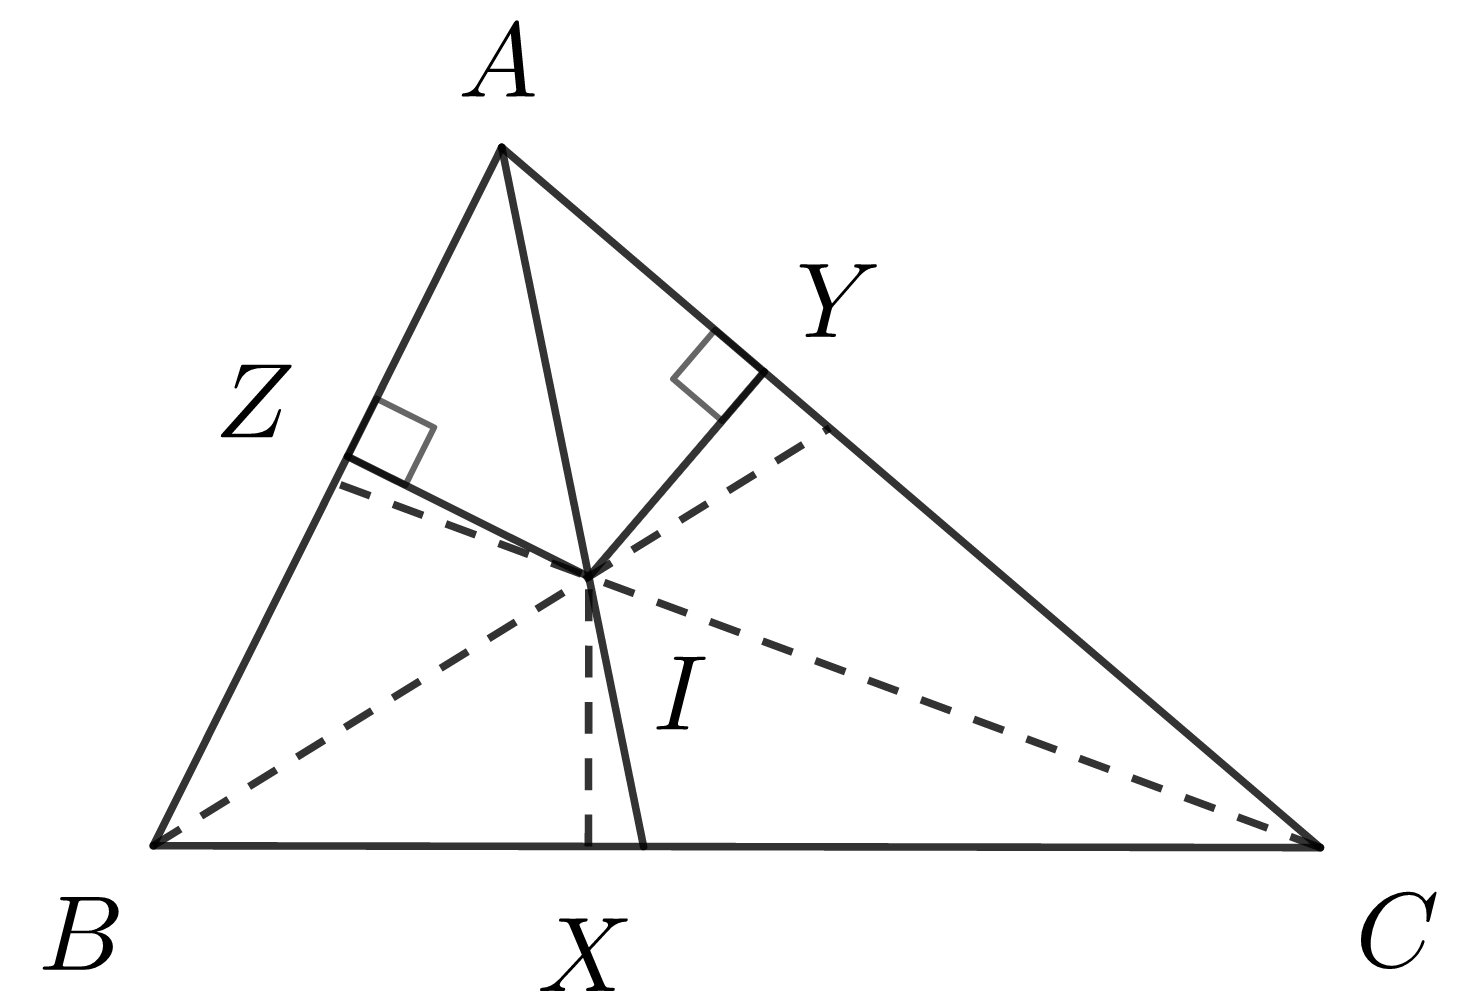
\includegraphics[scale=0.5]{bisectriz1.png} 
\end{center}
\end{tabular}
\\
\begin{tabular}{p{15.9cm}p{1cm}}
\\Sea $Z$ el pie de la perpendicular de $P$ sobre $AB$ y $Y$ es el pie de la perpendicular de $P$ sobre $CA$.
\\Por criterio de congruencia en los triángulos $AZP$ y $AYP$, $PZ=PY$. & (1)
\\Sea un punto $P$ dentro del ángulo $\angle CAB$ de un triángulo $ABC$, que cumpla que $PZ=PY$ donde $Y$ y $Z$ como los pies de la perpendicular de $P$ sobre $CA$ y $AB$, respectivamente.
\\Por definición y congruencia de triángulo L-A-L, $\angle PAZ = \angle PAY$. &(2) 
\\Por (2), se cumple el recíproco, es decir un punto $P$ que cumpla que $PZ=PY$ necesariamente un punto de la bisectriz interna. & \medskip(3)
\\Definimos por $b_a$, $b_b$, $b_c$ a las bisectrices internas de los ángulos en $A$, $B$, $C$ respectivamente
\\Sea $I$ el punto de intersección de las bisectrices $b_b$ y $b_c$ (hay punto de intersección, en caso contrario los ángulos en $B$ y $C$ del triángulo sumarían $180^{\circ}$).
\\Sean $X$, $Y$ y $Z$ los pies de las perpendiculares de $I$ sobre los lados $BC$, $CA$ y $AB$ respectivamente. 
\\Por estar $I$ en la bisectriz $b_c$ y (3), tenemos que $IX=IY$ y por estar $I$ en la bisectriz $b_b$, tenemos que $IX=IZ$. &\medskip(4)
\\Por (4), $I$ cumple $IY=IZ$. &(5)
\\Por (5), $I$ se encuentra en la bisectriz $b_a$.& (6)
\\Por definición y (6), las bisectrices internas concurren en $I$.
\end{tabular}
\subsection*{8. Teorema.}
Las mediatrices de los lados de un triángulo son concurrentes.\\
\begin{tabular}{p{15.9cm}p{1cm}}
\subsection*{Demostración:}
\begin{center}
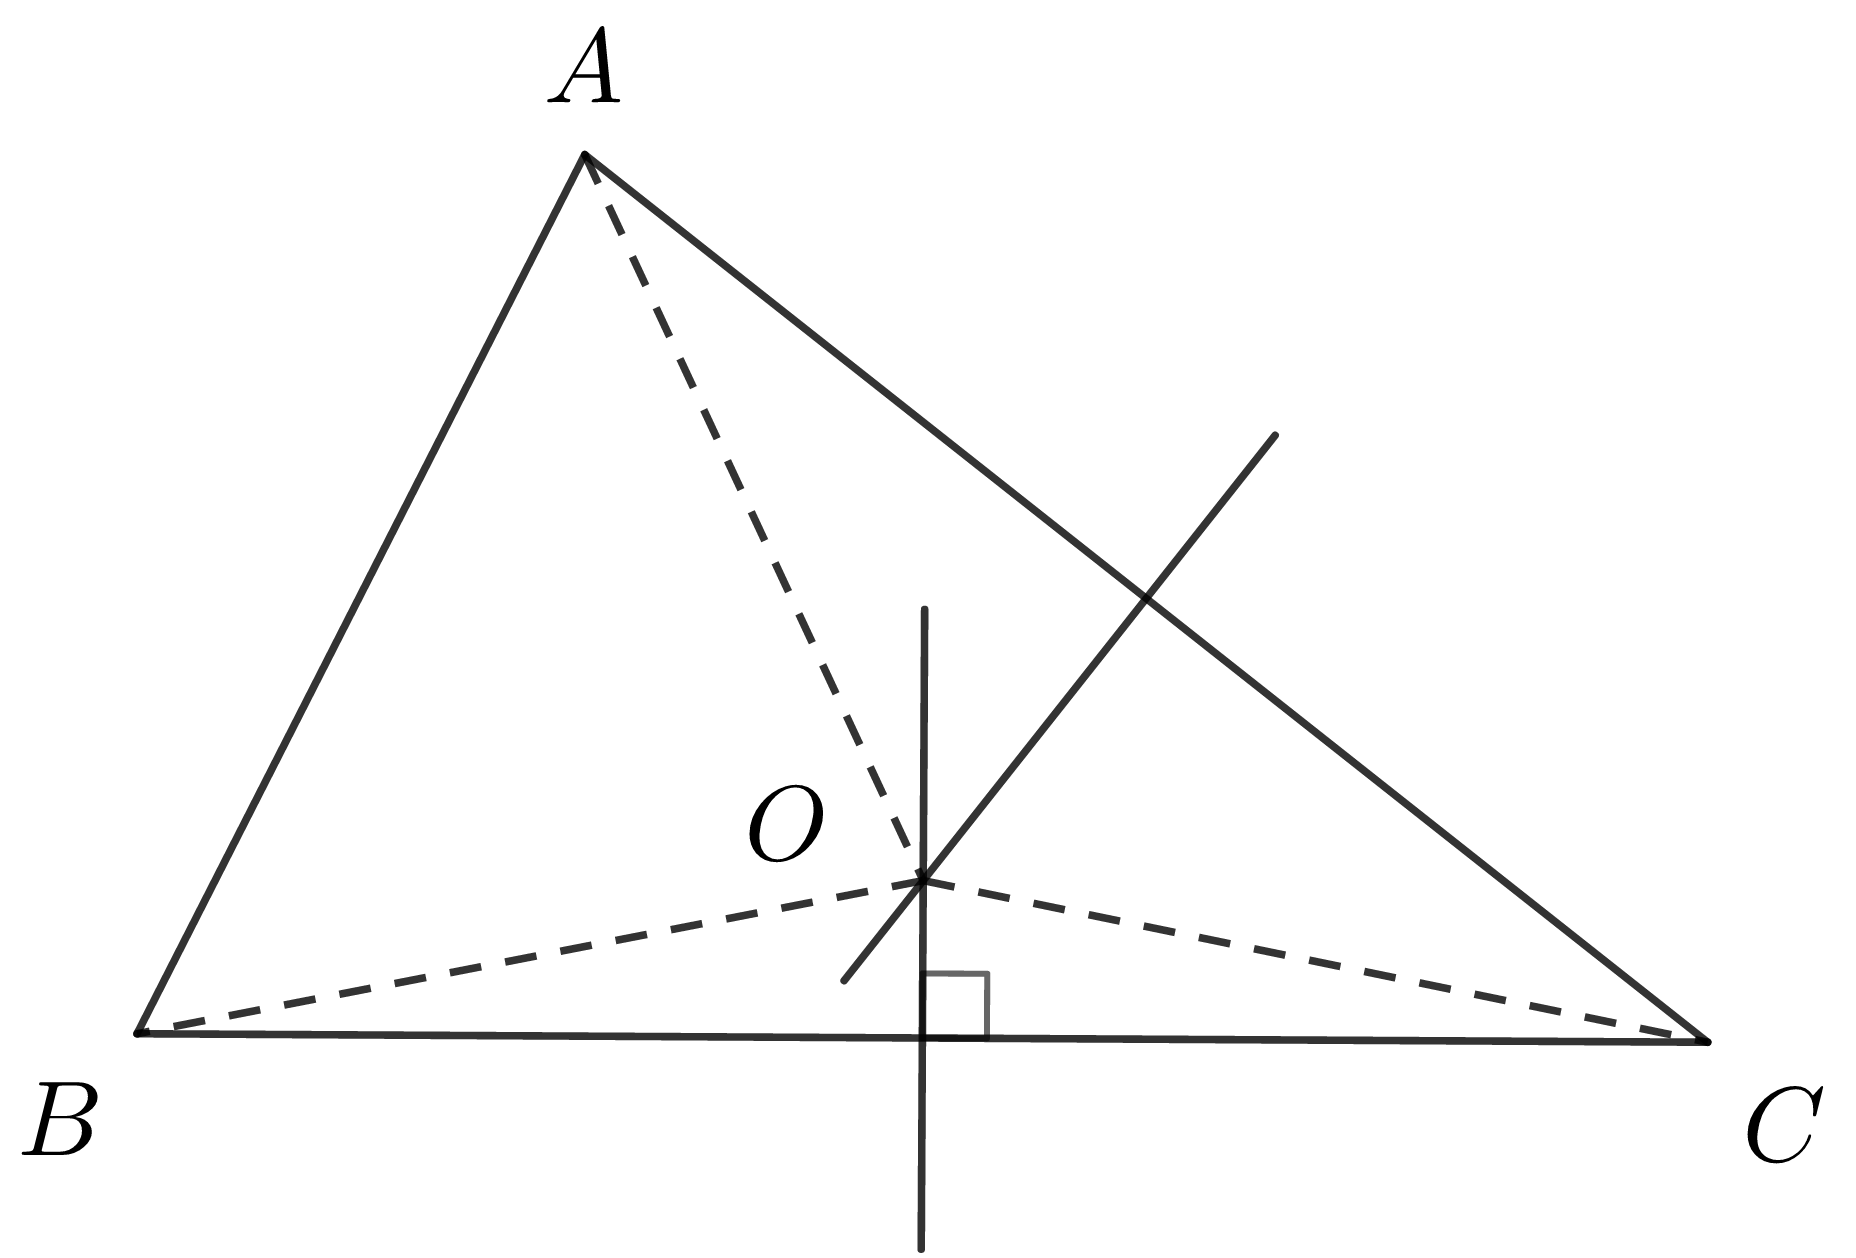
\includegraphics[scale=0.6]{mediatriz.png} 
\end{center}
\\Sean $l_a$ y $l_b$ las mediatrices de los lados $BC$ y $CA$ del triángulo $ABC.$
\\Si $l_a$ y $l_b$ son paralelas entonces también $BC$ y $CA$ son paralelos, lo cual es una contradicción. &\medskip(1)
\\Por (1), las mediatrices se intersectan y sea $O$ el punto de intersección de estas mediatrices. & (2) 
\\Por definición, $O$ está en $l_a$ &(3)
\\Por (3) y congruencia de triángulo, $OB=OC$ &(4)
\\ Análogo a (4) en $l_b$, $OA=OC$. &(5)
\\Por (4) y (5), $OA=OB$. &(6)
\\Por (6), $O$ está en la mediatriz de $AB$. &(7)
\\ Por (7), las mediatrices concurren, que se denota por $O$, se conoce como el circuncentro del triángulo $ABC$. 
\end{tabular}
\subsection*{9. Teorema.}
Las alturas de un triángulo son concurrentes.
\subsection*{Demostración:}
\begin{center}
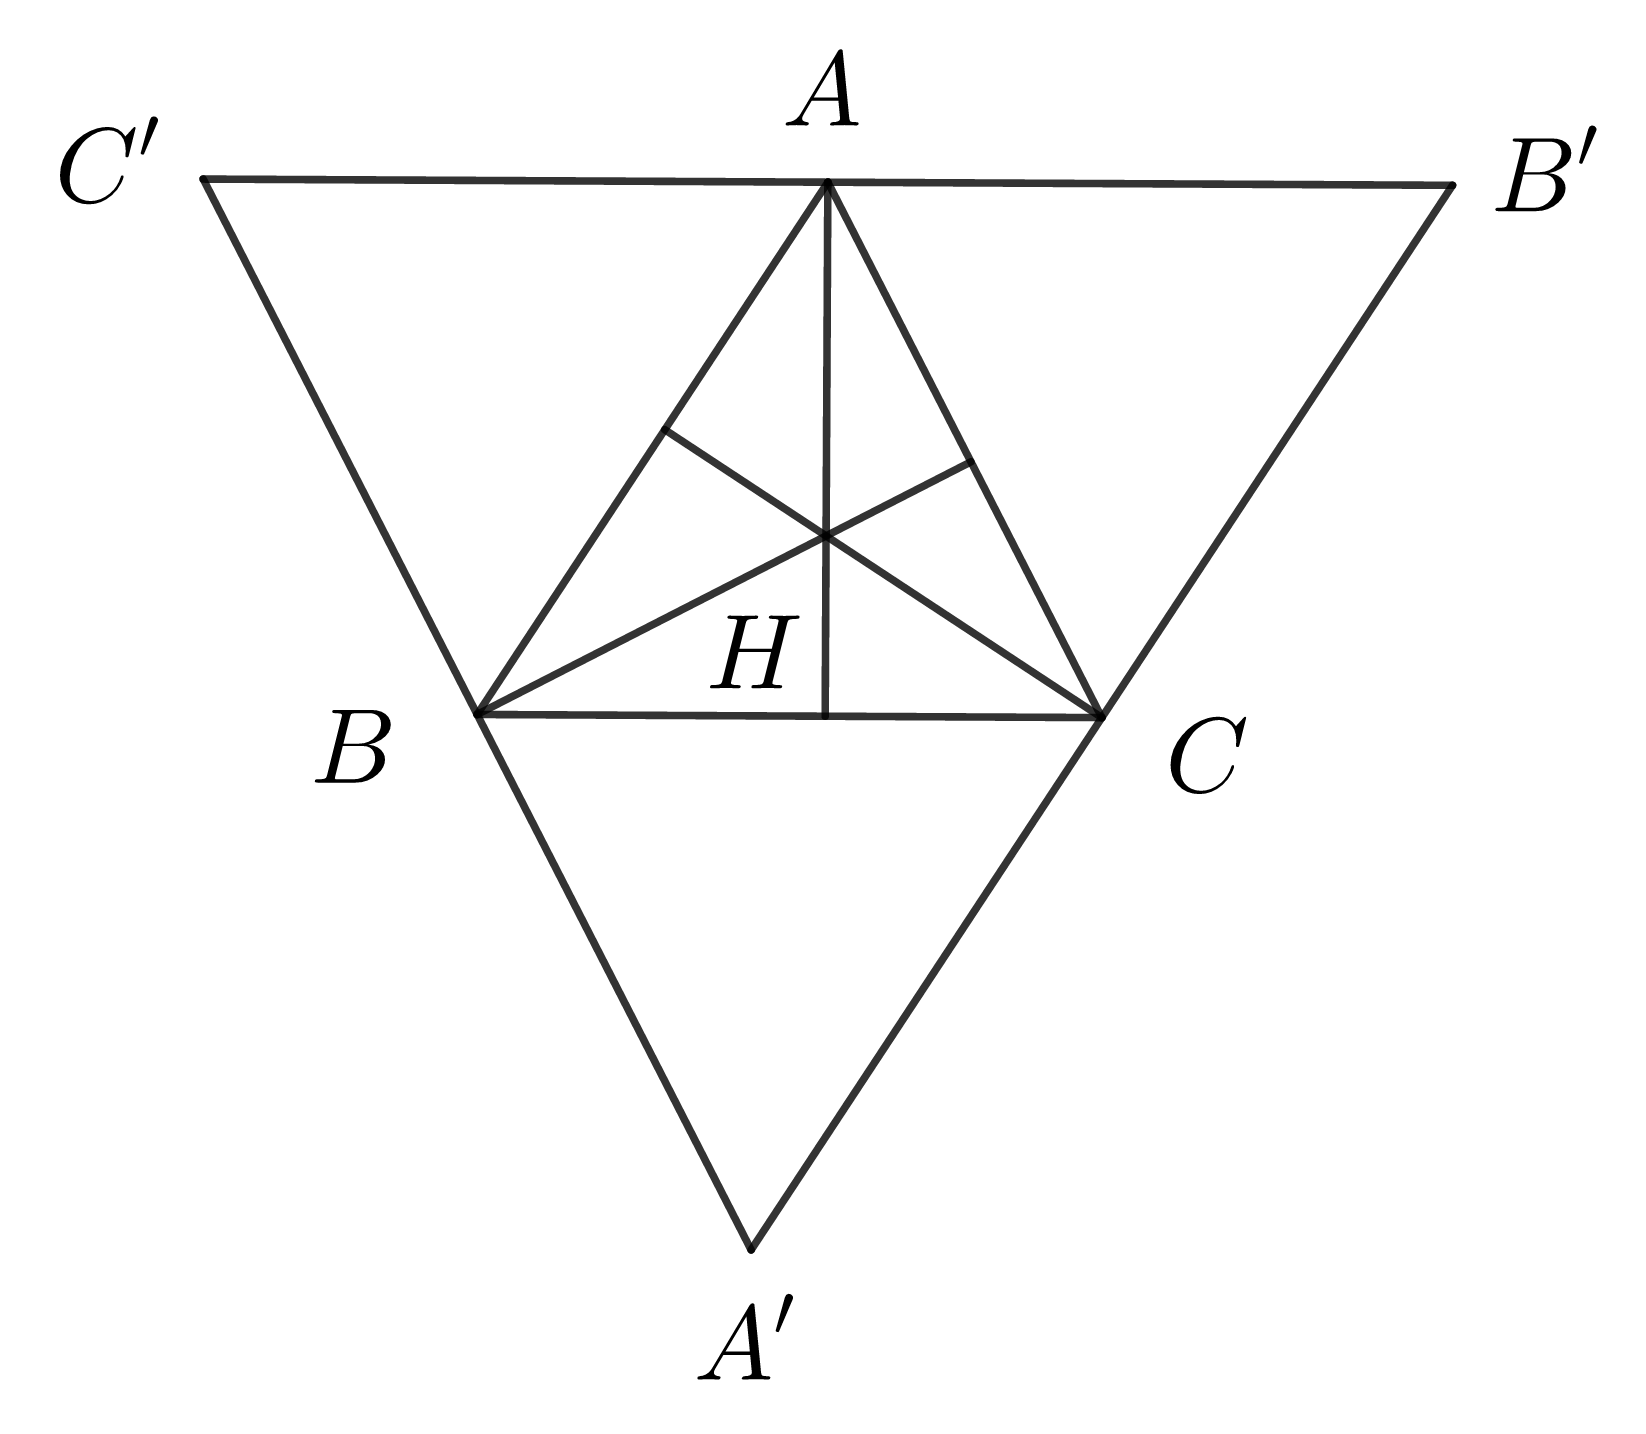
\includegraphics[scale=0.6]{alturas.png} 
\end{center}
\begin{tabular}{p{15.9cm}p{1cm}}
Sea $ABC$ el triángulo y trazamos por cada vértice la recta que es paralela al lado opuesto de tal vértice, estas rectas paralelas determinan un triángulo $A'B'C'$.
\\Por definición; $ABCB'$, $AC'BC$ y $ABA'C$ son paralelogramos. &(1) 
\\Por (1); tenemos que $A$, $B$ y $C$ son puntos medios de $B'C'$,  $C'A'$ y $A'B'$ respectivamente& (2)
\\Por (2), las alturas de $ABC$ son las mediatrices del triángulo $ABC$ &(3)
\\Por (3) y saber que las mediatrices concurren, las alturas que son mediatrices son concurrentes. &\medskip(4)
\\Por (4), las alturas de $ABC$ son concurrentes.
\end{tabular}
\subsection*{10.1. Teorema de la medida del ángulo inscrito.}
La medida de un ángulo inscrito en una circunferencia es igual a la mitad del arco comprendido entre sus lados, es decir, es la mitad del ángulo central que abre del mismo arco.
\subsection*{Demostración:}
\textbf{Primer caso.}
\begin{center}
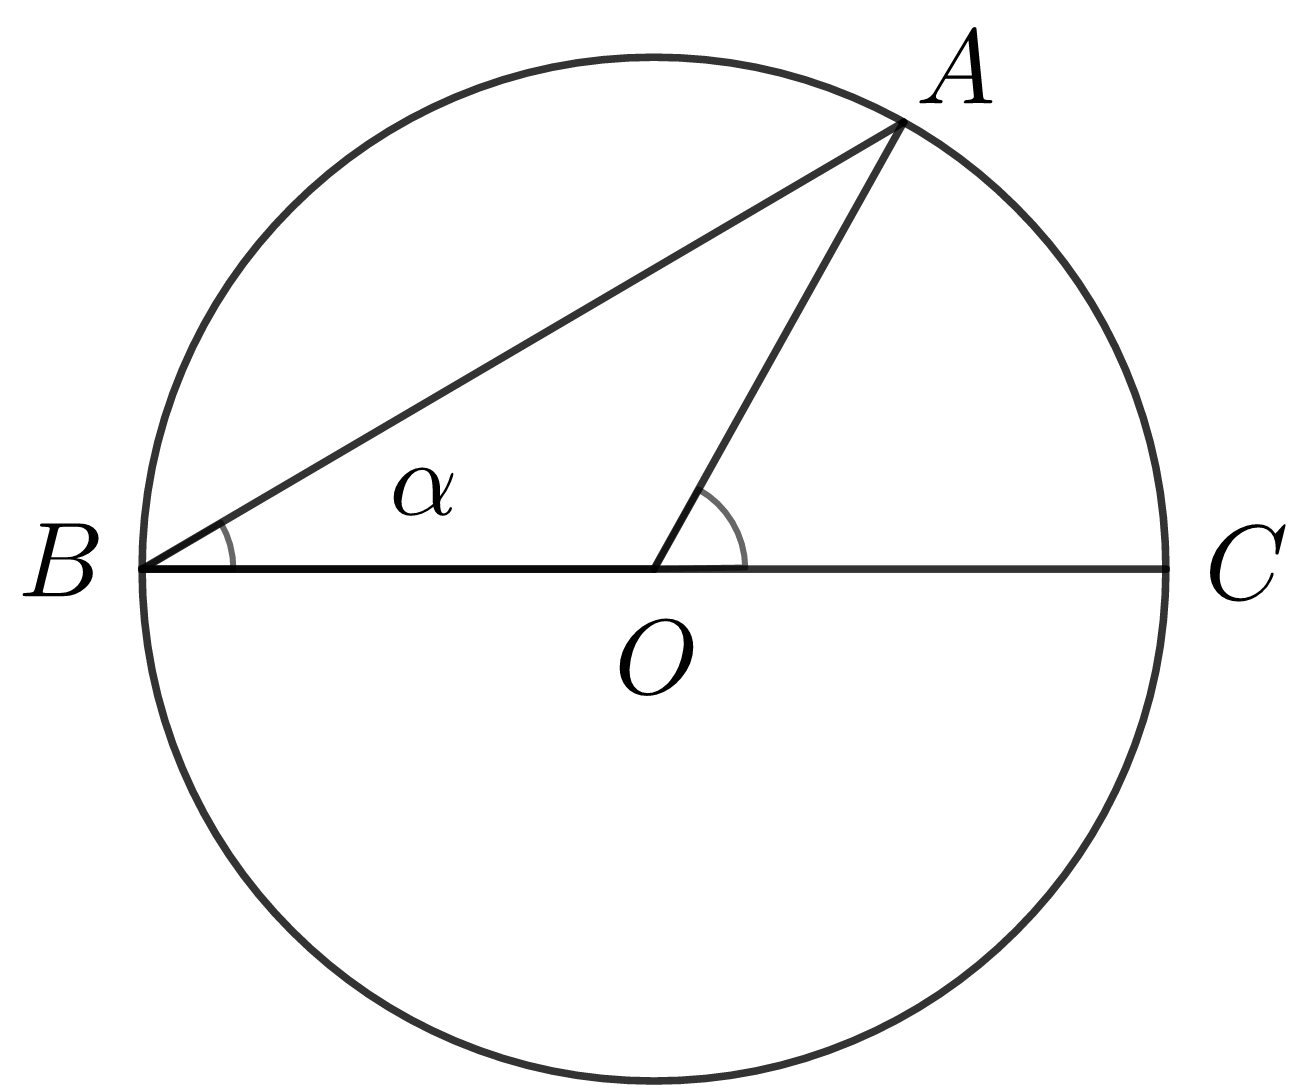
\includegraphics[scale=0.6]{circulo.png} 
\end{center}
\begin{tabular}{p{15.9 cm} p{1cm}}
Un lado del ángulo inscrito pasa por el centro de la circunferencia 
\\Definimos como $\alpha =\angle ABC$ que es el ángulo inscrito y que el centro de la circunferencia $O$ se encuentra sobre $BC$. 
\\Por hipótesis y definición, el triángulo $ABO$ es isósceles. &(1)
\\Por (1), $\angle ABO = \angle BAO = \alpha$ &(2)
\\Por suma de ángulo internos de un triángulo, la medida del ángulo exterior al vértice $O$ del triángulo $ABO$ es la suma de los otros dos ángulos interiores. &\medskip(3)
\\Por (3), tenemos que $\angle AOC =2 \alpha$ como queríamos demostrar.
\end{tabular}\\\\
\textbf{Segundo caso.}
\begin{center}
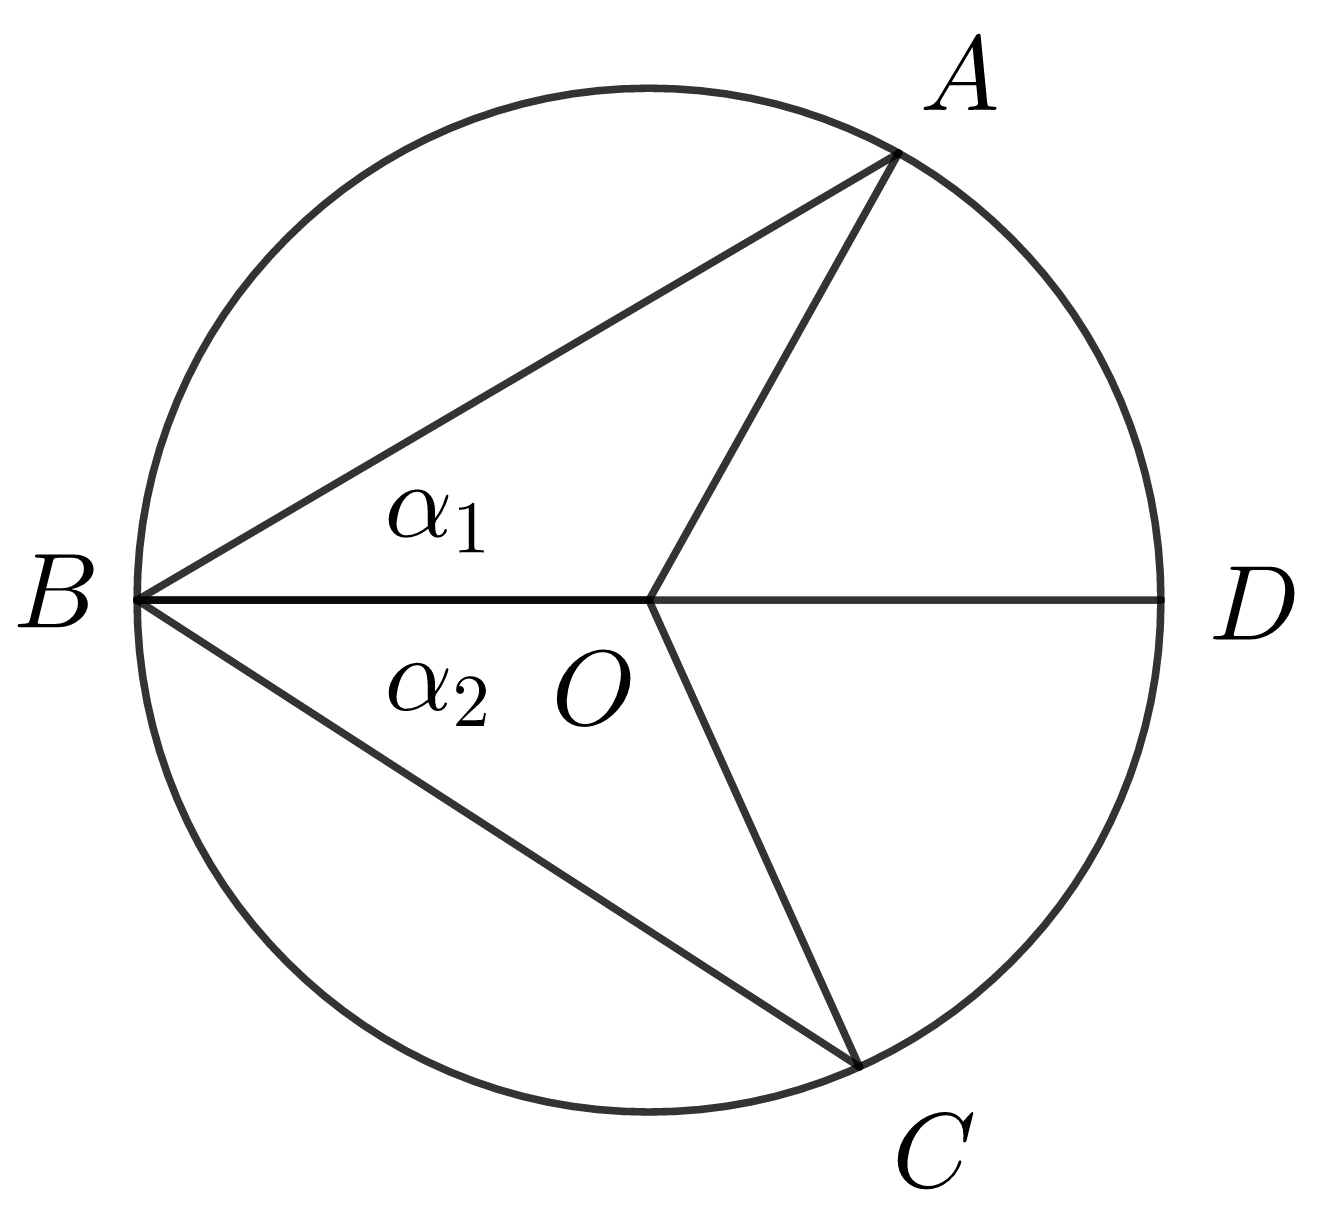
\includegraphics[scale=0.6]{circulo 1.png} 
\end{center} 
\begin{tabular}{p{15.9 cm} p{1cm}}
El centro de la circunferencia es un punto interior del ángulo
\\Trazamos la cuerda $BD$ que pase por el centro $O$. 
\\Definimos el ángulo $\alpha =\angle ABC$, el cual queda divido en dos partes por $BD$.
\\Sea $\alpha_1 = \angle ABD$ y $\alpha _2= DBC$. 
\\Por el primer caso y definición, $\angle AOD = \angle AOD + DOC =2 \alpha _1 + 2 \alpha _2$ y $\angle DOC= 2 \alpha _2$. &(1)
\\Por (1), $\angle AOC = \angle AOD + \angle DOC = 2 \alpha _1 + 2 \alpha _2 = 2 \alpha $.
\\\\\textbf{Tercer caso.}
\begin{center}
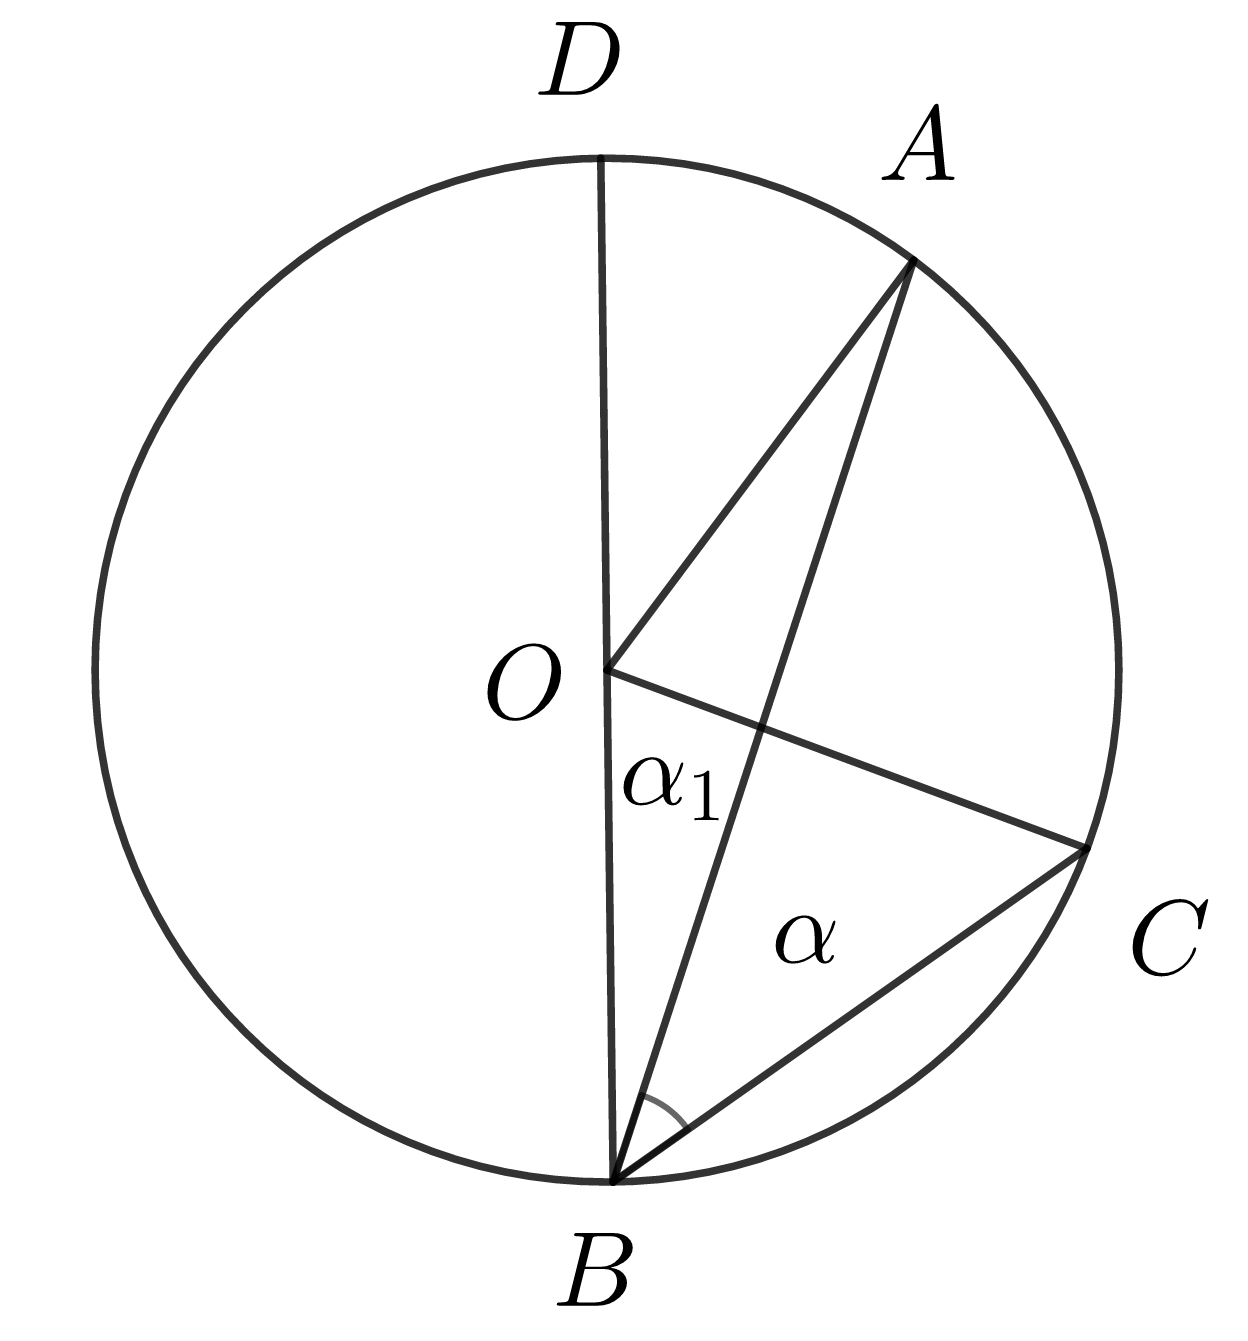
\includegraphics[scale=0.6]{circulo 2.png} 
\end{center} 
El centro de la circunferencia es un punto exterior del ángulo.
\\Trazamos el diámetro $BD$ y definimos $\alpha _1 = \angle ABC$ y $\alpha _2 = \angle CDB$.
\\Por hipótesis, definición y suma de ángulos internos del triángulo; $\alpha = \angle ABC= \alpha _2 - \alpha_1$ &(1)
\\Por el primer caso y definición, $\angle AOD= 2\alpha _1 $ y $\angle COD= \alpha _2$. &(2)
\\Por (1) y (2), $\angle COA = \angle COD - \angle AOD= 2 \alpha _2 - 2 \alpha_1= 2 \alpha$ como queríamos demostrar.
\end{tabular}
\subsection*{10.2. Teorema de la medida del ángulo semi-inscrito.}
Todo ángulo semi-inscrito es igual a la mitad del ángulo central que abarca el mismo arco.
\subsection*{Demostración:}
\begin{center}
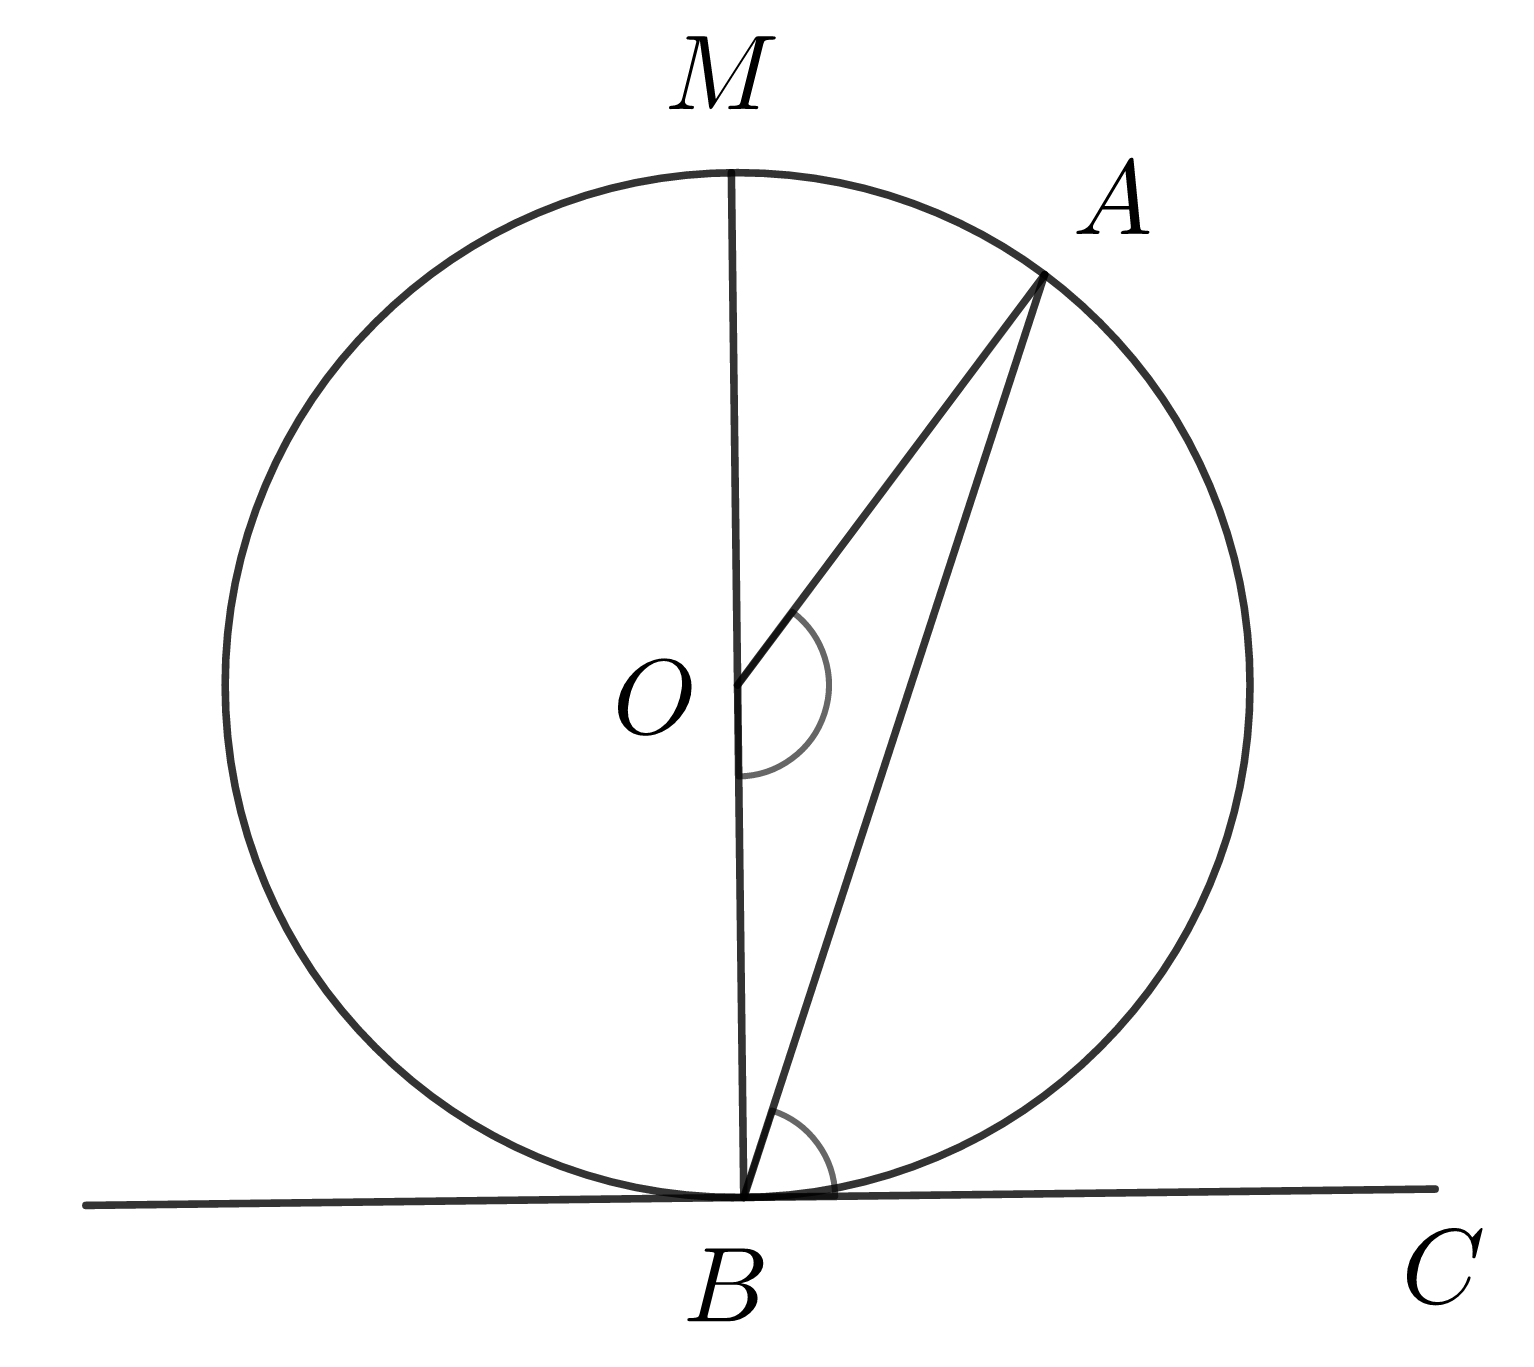
\includegraphics[scale=0.6]{circulo 3.png} 
\end{center}
\begin{tabular}{p{15.9 cm} p{1cm}}
Prolonguemos el radio  $BO$ para formar un diámetro $BM$. 
\\Por ser $BC$ la tangente, el ángulo $MBC$ es recto. &(1)
\\Por (1), $\angle MBC = \dfrac{\angle MOB}{2}$ &(2)
\\Por el teorema del ángulo inscrito, $\angle MBA = \dfrac{\angle MOA }{2}$&(3)
\\Por (1) y (2), $\angle ABC = \angle MBC - \angle MBA= \dfrac{\angle MOB}{2}-\dfrac{\angle MOA}{2}=\dfrac{\angle AOB}{2}$ que es lo que queríamos demostrar.
\end{tabular}
\subsection*{11. Teorema.}
Un cuadrilátero convexo es cíclico si y solamente si tiene dos ángulos opuestos suplementarios.\\
\begin{tabular}{p{15.9 cm} p{1cm}}
\subsection*{Demostración:}
\begin{center}
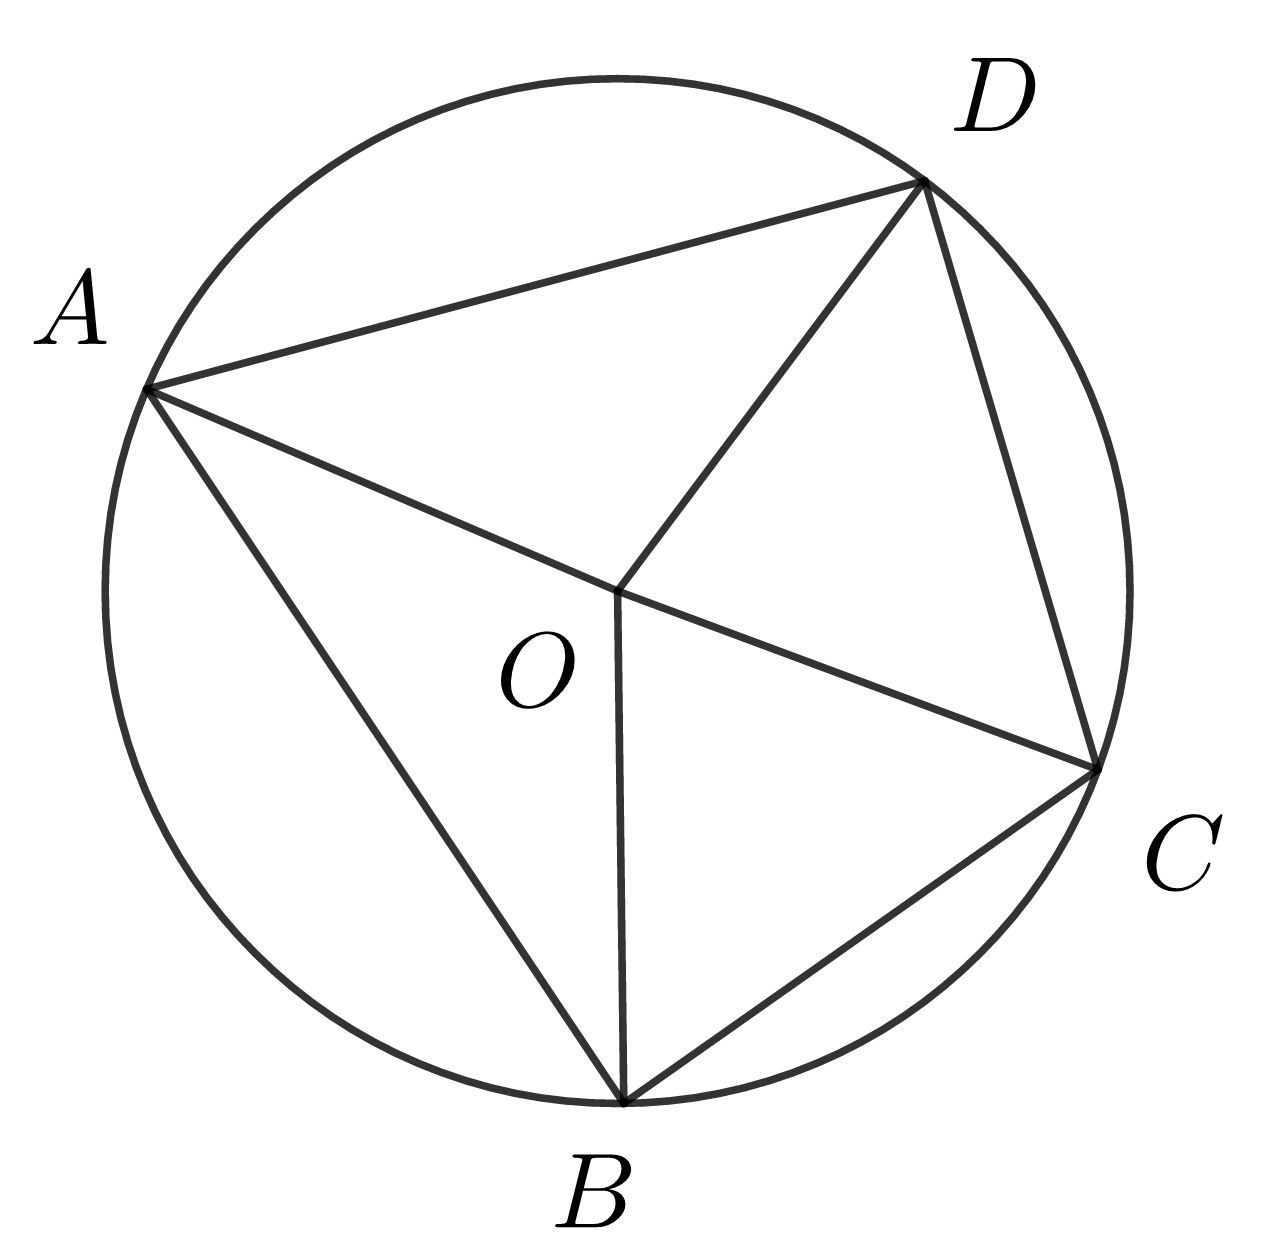
\includegraphics[scale=0.6]{ciclico.png} 
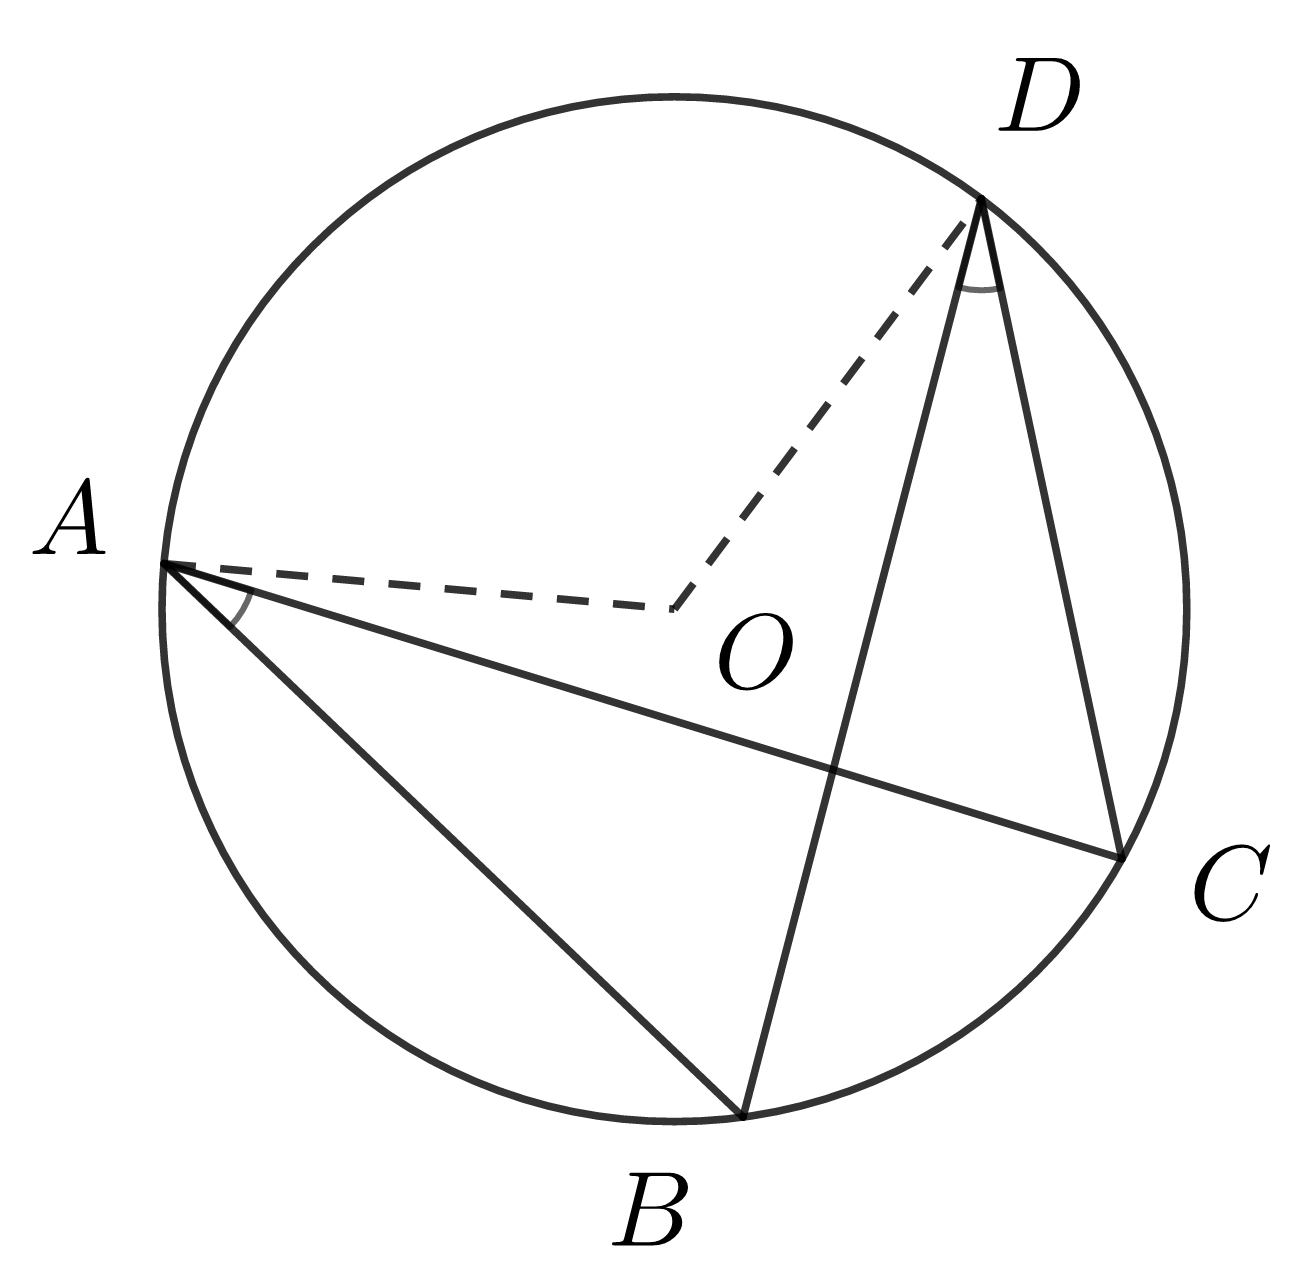
\includegraphics[scale=0.6]{ciclico1.png} 
\end{center}
Sea $ABCD$ un cuadrilátero convexo y sea $O$ su centro.
\\Si el cuadrilátero $ABCD$ está inscrito en una circunferencia entonces por el teorema del ángulo inscrito, los ángulos inscritos que abren de un mismo tienen la misma medida. & \medskip(1)
\\Por (1), $\angle A= \angle BAD= \dfrac{1}{2}\angle BOD$ y $\angle C= \angle DCB = \dfrac{1}{2}\angle DOB$ &(2)
\\ Por (2), $\angle BAD + \angle DCB = \dfrac{1}{2}( \angle BOD + \angle DOB)=180^\circ$ & (3)
\\Recíprocamente, supongamos que los ángulos en $A$ y en $C$ del cuadrilátero convexo $ABCD$ son suplementarios y consideramos el circuncírculo del triángulo $BCD$. & \medskip (4)
\\Por (1) y (4), los puntos $P$ que se encuentran sobre el arco $DB$ opuesto al vértice $C$, cumplen que el $\angle BPD$ es suplementario al $\angle DCB$. &\medskip(5)
\end{tabular}
\begin{center}
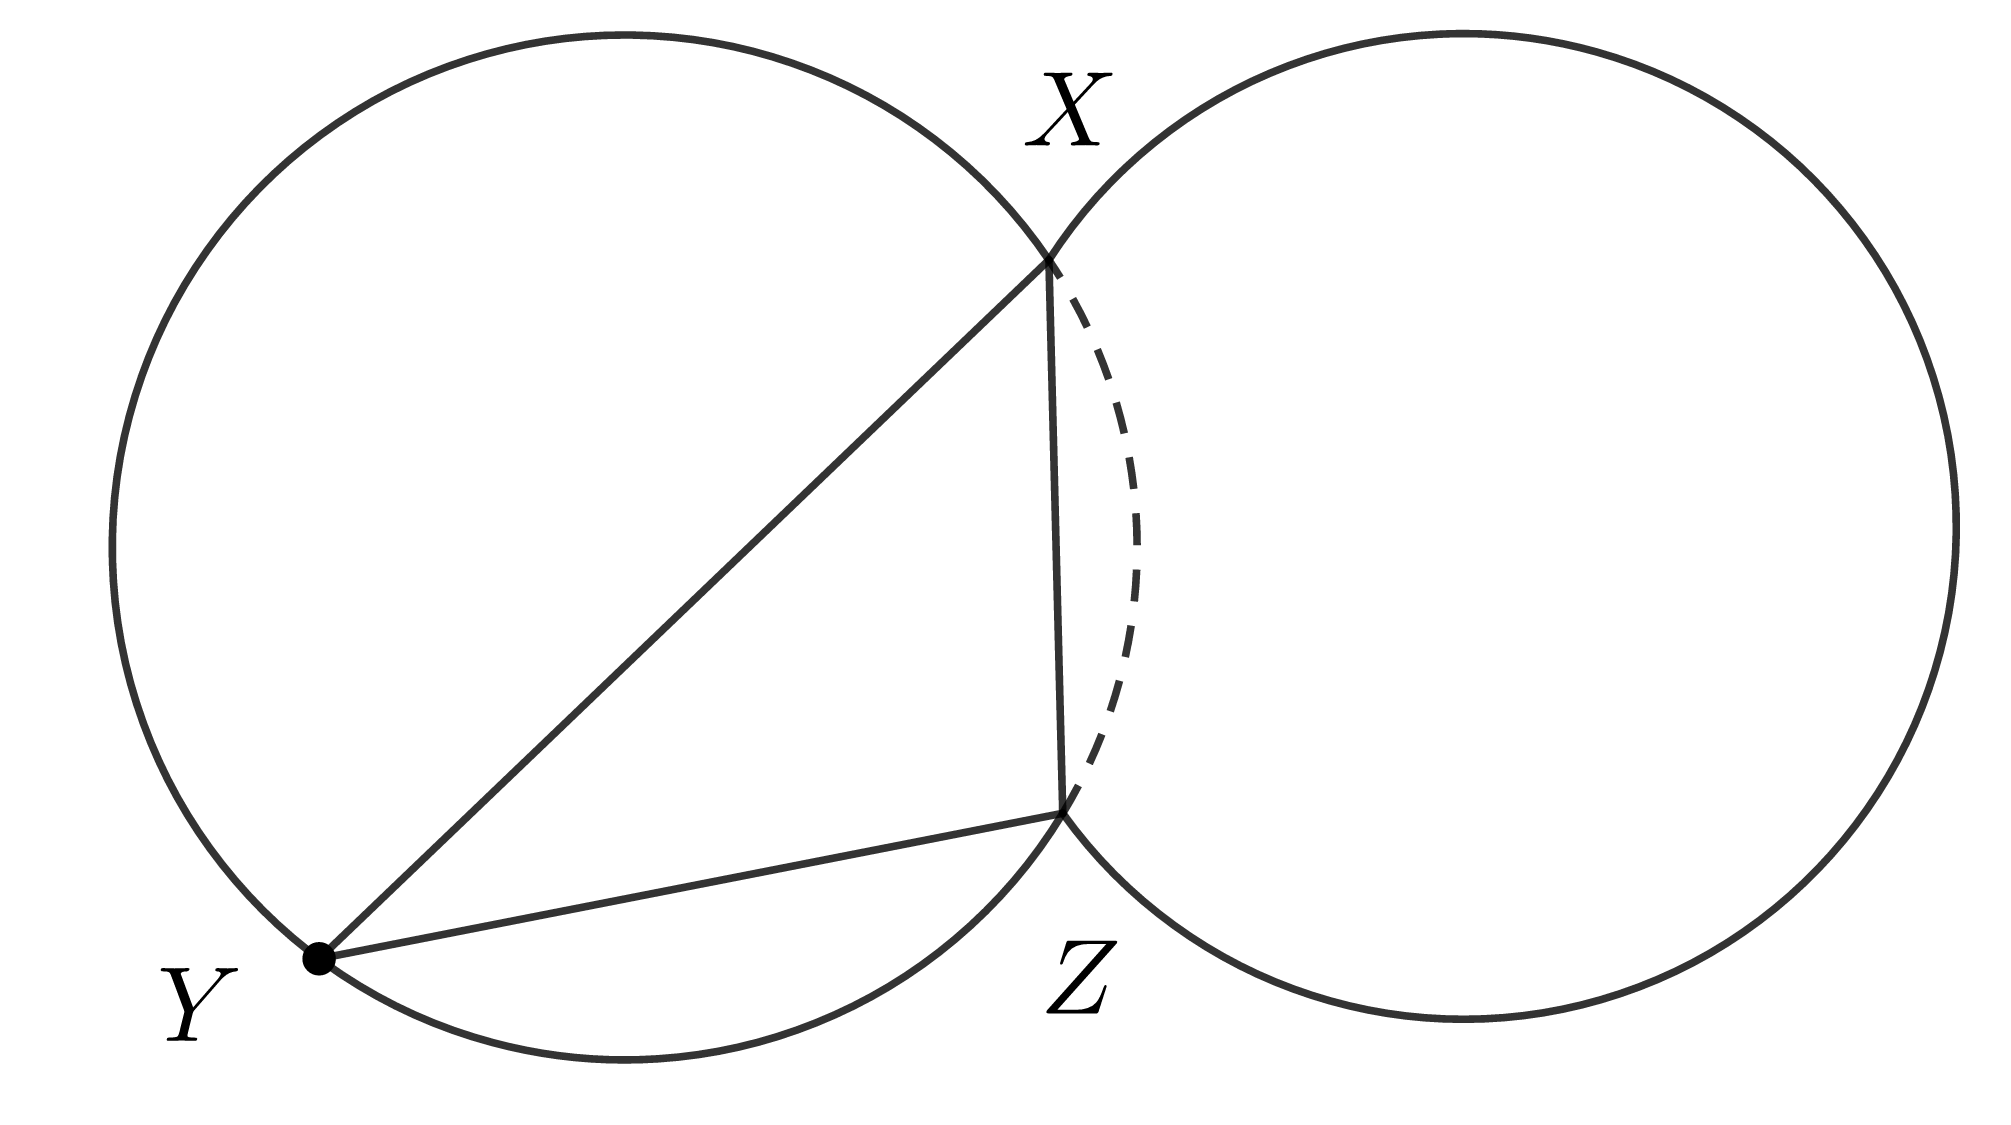
\includegraphics[scale=0.6]{ciclico 2.png} 
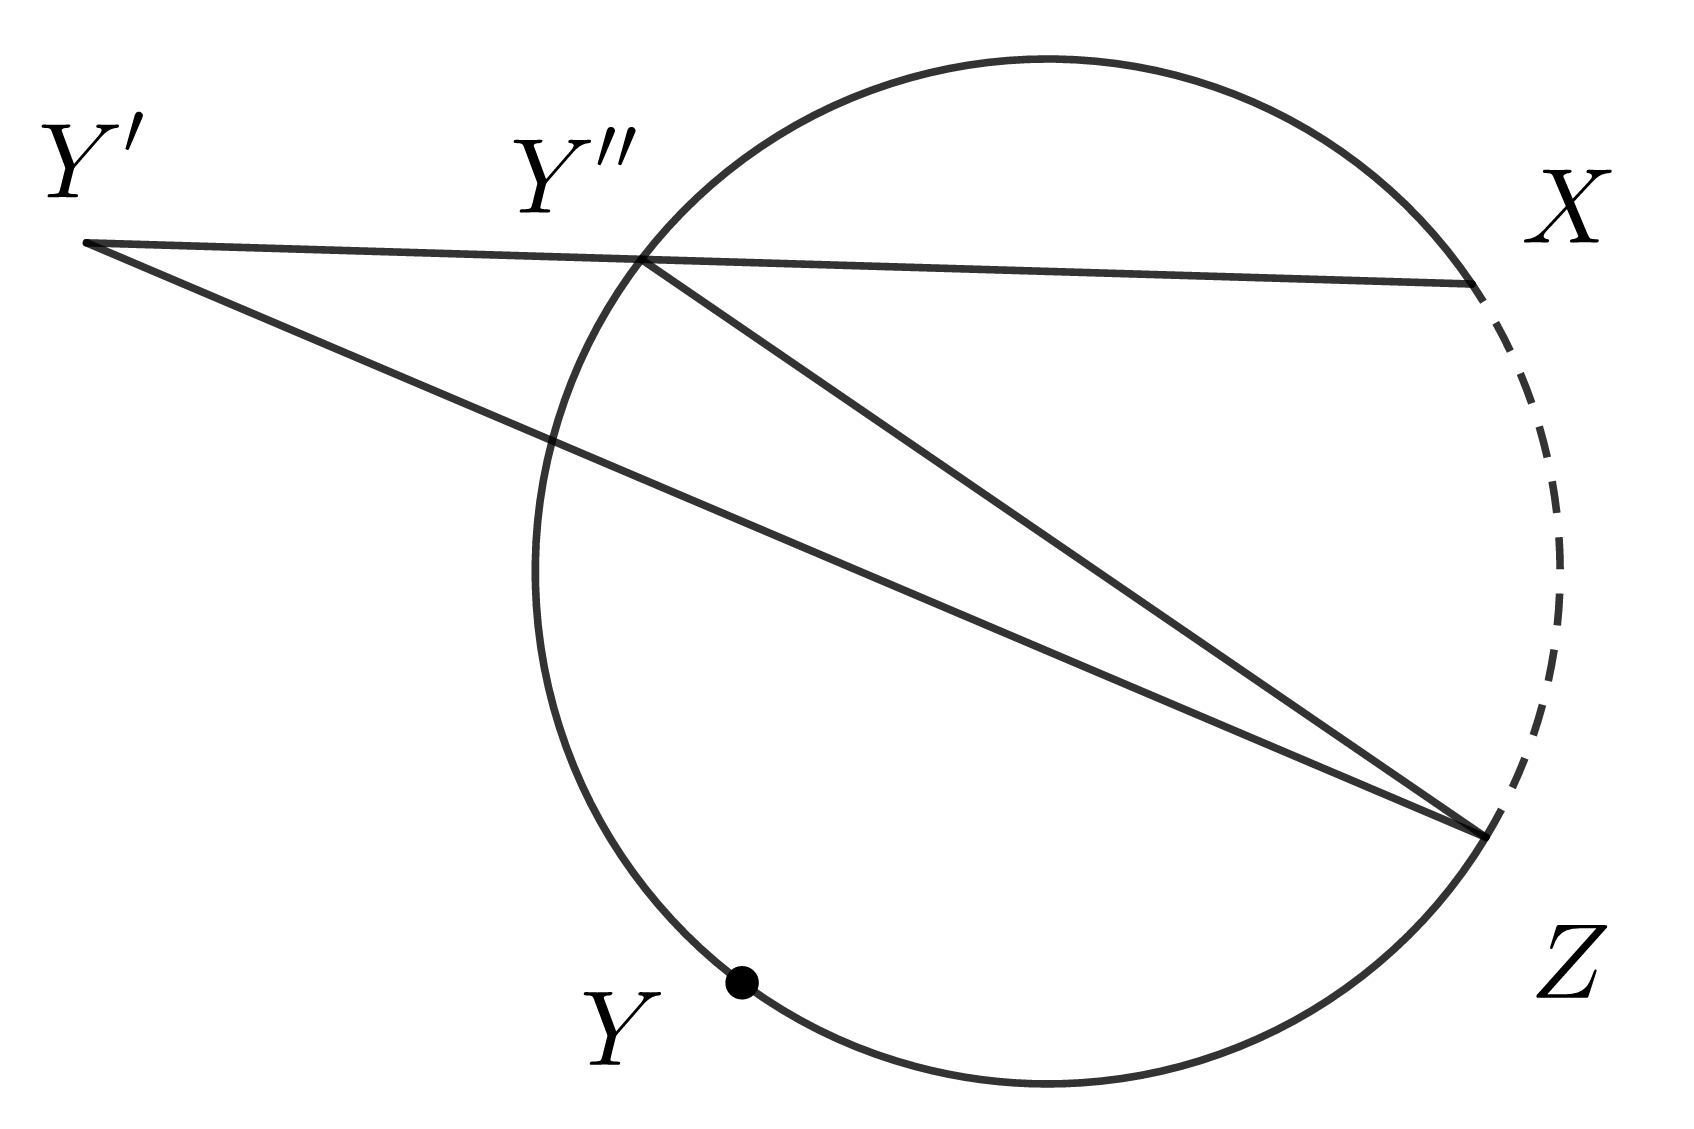
\includegraphics[scale=0.6]{ciclico 3.png} 
\end{center}
\begin{tabular}{p{15.9 cm} p{1cm}}
\\Supongamos que $Y$ es un punto en el conjunto y construyamos el circuncirculo del triángulo $XYZ$. Los puntos $X$ y $Z$ dividen a la circunferencia en dos arcos, en uno de ellos se encuentra $Y$.
\\Por (1), los puntos del arco que contiene a $Y$ son puntos del conjunto que cumple que $\angle XYZ$ es constante. & \medskip(6)
\end{tabular}
\begin{tabular}{p{15.9 cm} p{1cm}}
\\Consideramos el arco de circunferencia que resulta de reflejar el arco anterior con respecto a la recta por $X$ y $Z$, estos pertenecen también al conjunto que cumple que $\angle XYZ$ es constante.&\medskip\medskip(7)
\\Por (6) y (7), los puntos del conjunto son solamente los puntos de estos arcos.
\\Supongamos que $Y'$ es un punto del conjunto y que se encuentra en el mismo lado de $Y$ con respecto a la recta por $X$ y $Z$, caso contrario se considera su reflejo en el otro arco con respecto a $XZ$
\\Por definición de $Y'$, $\angle XY'Z= \angle XYZ$ & (8)
\\Si $Y'$ no se encuentra sobre el circuncirculo del triángulo $XYZ$, llamamos $Y"$ al punto de intersección de $XY'$ con el circuncírculo.
\\Por (1), $\angle XY"Z= \angle XYZ$. &(9)
\\Por (8) y (9), $Y'=Y"$.&(10)
\\Por el (5) y (10), los puntos que cumplen que el $\angle BPD$ es suplementario al $\angle DCB$ son únicos.&(11)
\\Por (11), $A$ se encuentra el arco $DB$ &(12)
\\Por (12), $ABCD$ es cíclico. &(13)
\\Por (3) y (13), se cumple lo que queríamos demostrar.
\end{tabular}
\subsection*{12. Ley del paralelogramo.}
La suma de los cuadrados de las diagonales de un paralelogramo es igual a la suma de los cuadrados de sus lados, es decir, si $d_1$ y $d_2$ son las diagonales y $a, b$ los lados, entonces tenemos que 
$$d_1^2 + d_2^2=2a^2+2b^2$$
\subsection*{Demostración:}
\begin{center}
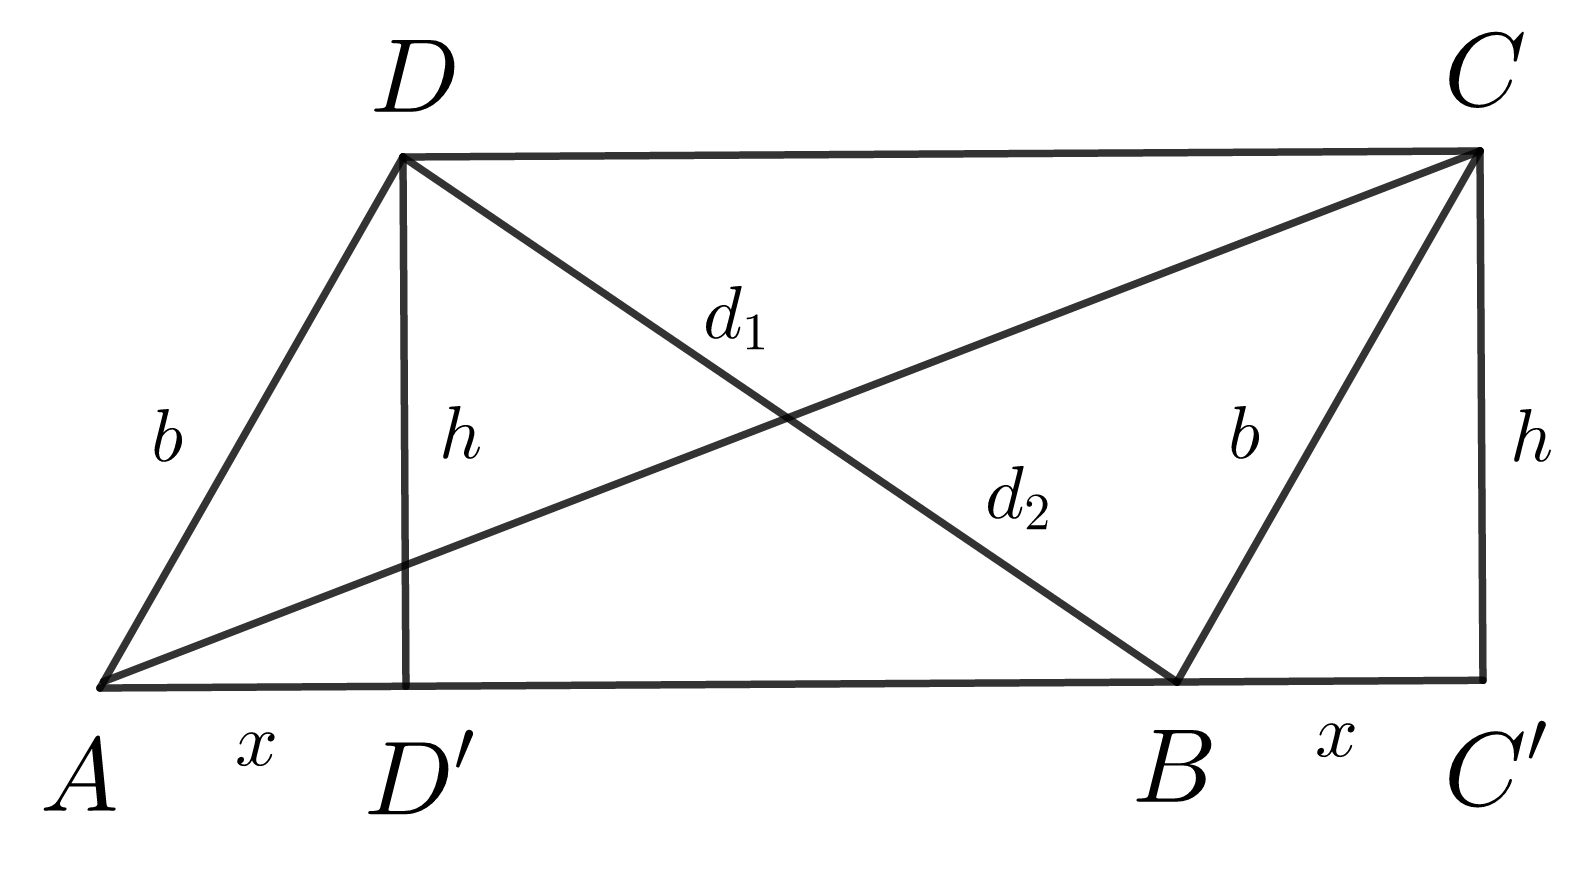
\includegraphics[scale=0.7]{paralelogramo.png} 
\end{center}
\begin{tabular}{p{15.9 cm} p{1cm}}
Sea $ABCD$ un paralelogramo con diagonales $d_1$ y $d_2$ y lados $AB=DC=a$, $DA=CB=b$. Y sean $D'$ y $C'$ los pies de las perpendiculares sobre $AB$ de $D$ y $C$, respectivamente.
\\Se construye los triángulos $BDD'$ y $AC'C$ como se muestra en la figura.
\\Por hipótesis y congruencia de triángulos, $CC'=DD'=h$ y $AD'=BC'=x$.
\\Por el teorema de Pitágoras y lo anterior, 
\end{tabular}
\begin{eqnarray}
b^2&=& h^2 +x^2 \\
d_1^2 &=&h^2 +(a-x)^2\\
d_2^2&=&h^2 +(a+x)^2
\end{eqnarray}
\begin{tabular}{p{15.9 cm} p{1cm}}
Por (2) y (3), $d_1^2 +d_2^2=h^2 +(a-x)^2+h^2 +(a+x)^2=2a^2+2(h^2+x^2)$ &(4)
\\Por (1) y (4), $d_1^2 +d_2^2=2a^2+2(h^2+x^2)=2a^2+2b^2$ & (5)
\\Por (5), $d_1^2 +d_2^2=2a^2+2b^2$
\end{tabular}
\subsection*{13. Teorema de la recta de Euler}
En un triángulo $ABC$ el ortocentro, el centroide y el circuncentro son colineales. La recta donde se encuentran estos puntos se conoce como la recta de Euler.\\
\begin{tabular}{p{15.9 cm} p{1cm}}
\subsection*{Demostración:}
\begin{center}
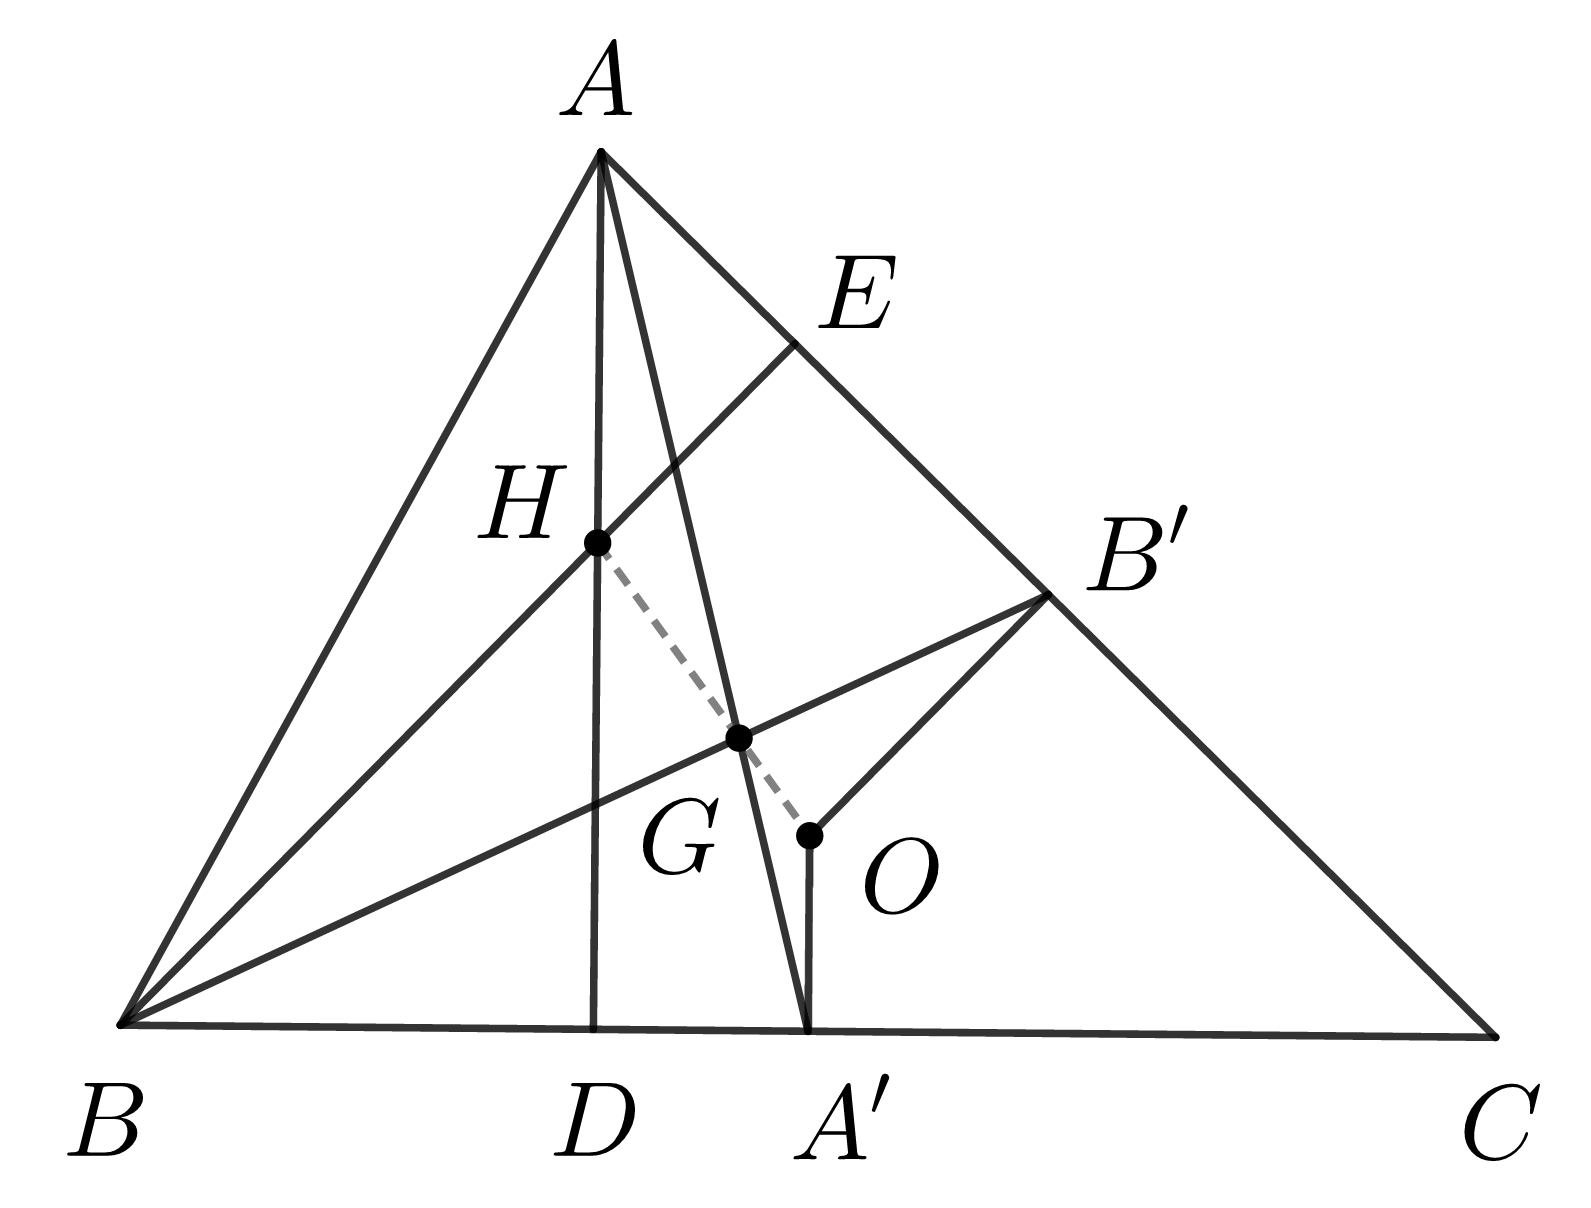
\includegraphics[scale=0.7]{recta_euler.png} 
\end{center}
Sean las medianas $AA'$, $BB'$ con centroide $G$, las alturas $AD$ y $BE$ con ortocentro $H$ y las mediatrices $OA'$ y $OB'$ con circuncentro $O$.
\\Por hipótesis, ser sus lados correspondientes  paralelos y semejanzas de triángulos $A-A-A$; los triángulos $ABH$ y $A'B'O$ son semejantes con razón de semejanza es $\dfrac{AB}{A'B'}=2$ &(1)
\\Por (1), $AH=2A'O$ &(2)
\\Por (2), $AH+2AO$. &(3)
\\Por ser $G$ el centroide, es conocido que $AG= 2GA'$. (4)
\\Por hipótesis, $AH$ y $A'O$ son ambas perpendiculares a $BC$ y son paralelas entre si. & (5)
\\Por (5), $\angle HAG= \angle OA'G$ &(6)
\\Por (6), ser $A$, $G$ ,$A'$ colineales y ángulo opuestos por un vértice; $H, G$ y $O$ son colineales. &(7)
\\Por (7) e hipótesis; el centroide, el ortocentro y el circuncentro son colineales.
\end{tabular}
\subsection*{14.1. Teorema de la Circunferencia de nueves puntos}
Los pies de las tres alturas de un triángulo, los puntos medios de los tres lados y los puntos medios de los segmentos que van de los vértices al ortocentro, están en una circunferencia de radio $\dfrac{1}{2}R$, donde $R$ es el radio del circuncentro del triángulo $ABC$.\\\\
\begin{tabular}{p{15.9 cm} p{1cm}}
\subsection*{Demostración:}
\begin{center}
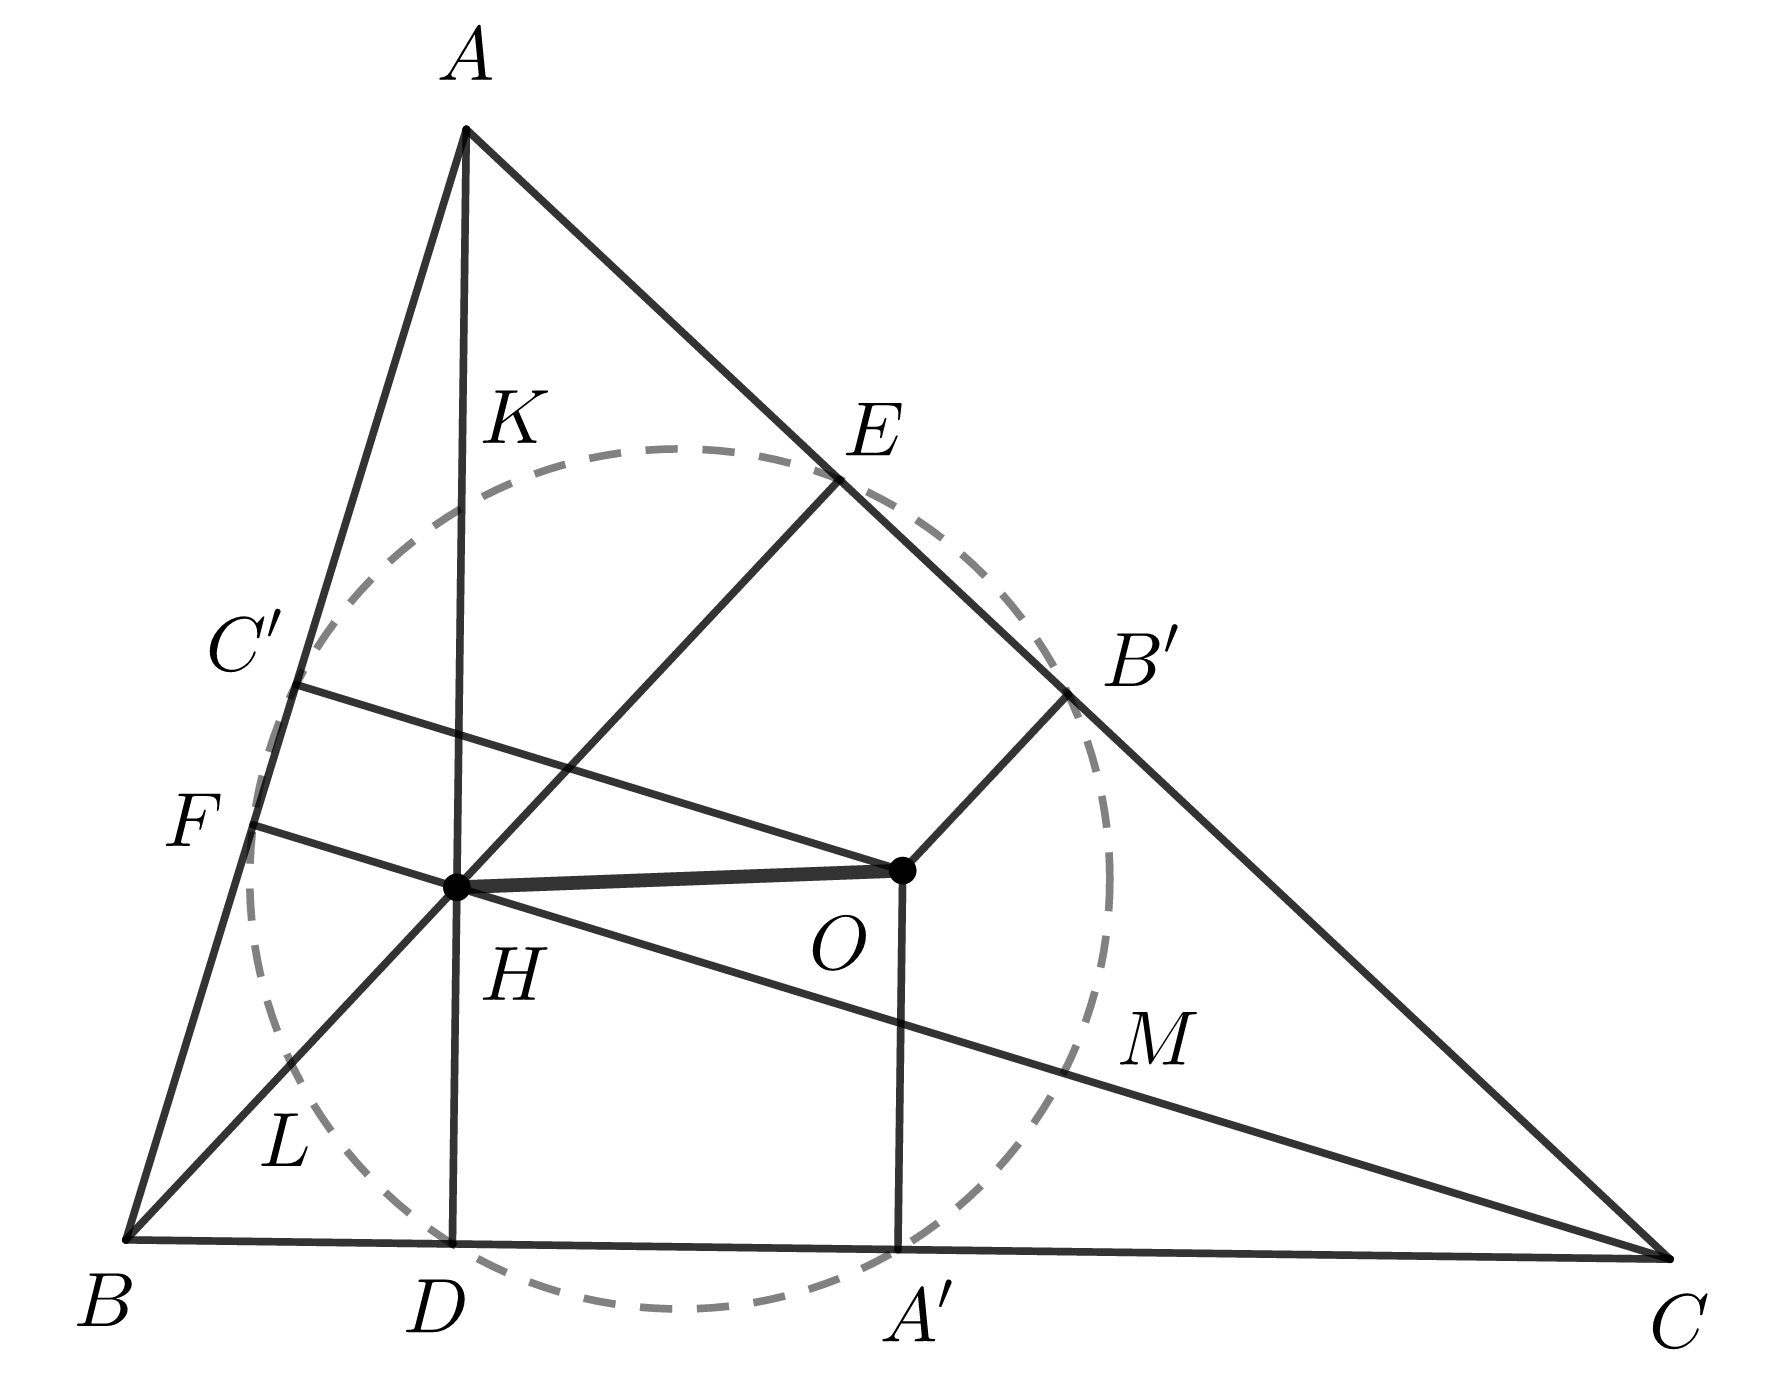
\includegraphics[scale=0.7]{circunferencia nueve.png} 
\end{center}
Sea $C'$, $A'$ y $B'$ son los puntos medios de los lados $AB$, $BC$ y $CA$, los puntos $K$, $L$ y $M$ son los puntos medios de los segmentos $AH$, $BH$ y $CH$ donde $H$ es un ortocentro. 
\\Por definición y paralela media, los segmentos $C'B'$ y $LM$ son paralelos al lado $BC$ &(1)
\\Por (1) y paralela media, $C'B'=LM=\dfrac{1}{2} BC$. &(2)
\\Análogamente, como $AH$ es un lado común de los triángulos $BAH$ y $CAH$, $C'L$ y $B'M$ son paralelos a $AH$ y $C'L=B'M=\dfrac{1}{2} AH$. &\medskip (3)
\\Por (1) y (3), $B'C'LM$ es un paralelogramo. &(4)
\\Por ser $BC$ y $AH$ perpendiculares y (4), $B'C'LM$ es rectángulo. &(5)
\\ Análogo a (5), $A'B'KL$ y $C'A'MK$ son rectángulos. &(6)
\\Es conocido que en un rectángulo las diagonales son iguales y se cortan en su punto medio. &\medskip(7)
\\Por (6) y (7), los rectángulos respectivos tienen una diagonal común. &(8)
\\ Por (8), $A'K$, $B'L$ y $C'M$ son diámetros de un mismo círculo (el circuncírculo del triángulo medial $A'B'C'$). &\medskip (9)
\\Por ser $\angle A'DK$ recto, el círculo con diámetro $AK$ pasa por $D$, análogamente pasa por $E$ y $F$. &\medskip(10)
\\Por (9) y (10), los puntos $A', B', C', D, E ,F, K, L, M$ pertenecen a una misma circunferencia. &\medskip(11)
\\Por ser $A'B'C'$ el triángulo medial, su circunradio es la mitad del circunradio del triángulo $ABC$ &\medskip(12)
\\Por (11) y (12), es lo que queríamos demostrar.
\end{tabular}
\subsection*{14.2. Teorema.}
El centro de la circunferencia de nueve puntos se encuentra en la recta de Euler y es el punto medio del segmento $HO$.\\\\
\begin{tabular}{p{15.9cm} p{1 cm}}
Usando los enunciados y datos de la solución anterior.
\\Sea $N$ el centro del circuncentro del triángulo $A'B'C'$.
\\Por (9), los puntos $K$, $L$ y $M$ son diametralmente opuestos a los puntos $A'$, $B'$ y $C'$. & (13)
\\Por (13), el triángulo $KLM$ se puede obtener rotando $180^\circ$ al triángulo $ABC$ y viceversa.  &(14)
\\Por (14) y definición, esta rotación intercambia los ortocentros $H$ y $O$.&(15)
\\Por (15), $N$ es el centro también es el circuncentro del triángulo $KLM$. & (16)
\\Por (16), $N$ es el centro de la circunferencia de Nueve puntos.
\end{tabular}
\subsection*{15. Teorema de Ceva.}
En un triángulo $ABC$ los puntos $D$, $E$, $F$ sobre los lados $BC$, $AC$, y $AB$, respectivamente. Las rectas $AD$, $BE$ y $CF$ concurren en un punto si y sólo si
$$\dfrac{BD}{DC}\cdot\dfrac{CE}{EA}\cdot\dfrac{AF}{FB}=1$$
\begin{center}
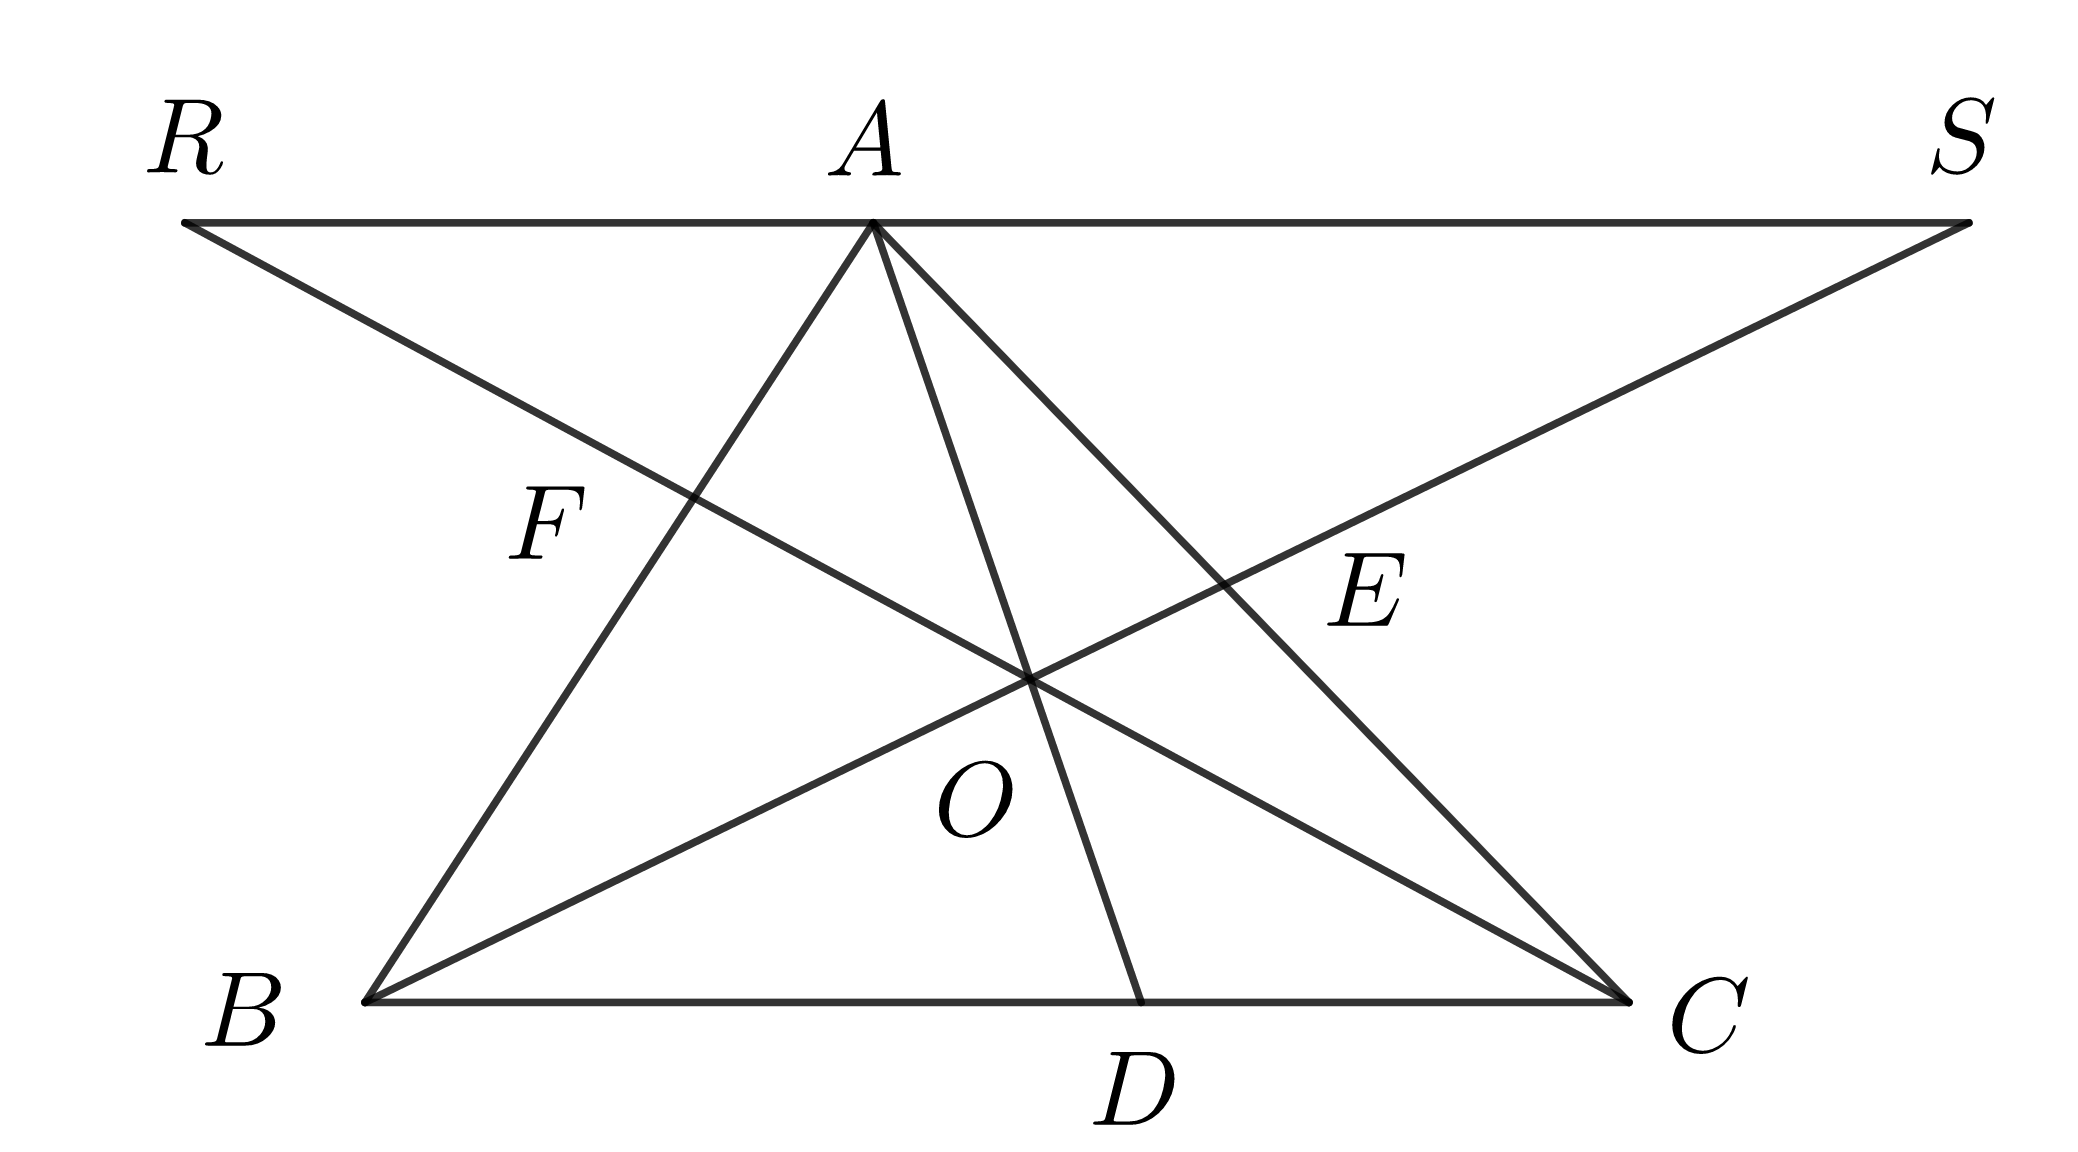
\includegraphics[scale=0.8]{Ceva.png} 
\end{center}
\begin{tabular}{p{15.9 cm} p{1cm}}
\subsection*{Demostración:}
Se traza una recta $l$ paralela a $BC$ que pasa por $A$. Sean $R$ y $S$ los puntos de intersección de $CF$ y $BE$ con $l$, respectivamente.
\\Por ser $l$ paralelo a $BC$, los triángulos $FAR$ y $FBC$ son semejantes& (1)
\\Por (1), $\dfrac{AF}{FB}=\dfrac{AR}{CB}$&(2) 
\\Análogamente; $\dfrac{CE}{EA}=\dfrac{CB}{SA}$, $\dfrac{BD}{DO}=\dfrac{SA}{AO}$, $\dfrac{DO}{DC}=\dfrac{AO}{AR}$&(3)
\\Por (3), $\dfrac{BD}{DC}=\dfrac{SA}{AR}$&(4)
\\Por (4) y (3), $\dfrac{BD}{DC}\cdot \dfrac{CE}{EA}\cdot \dfrac{AF}{FB}=\dfrac{SA}{AR}\cdot \dfrac{CB}{SA}\cdot \dfrac{AR}{CB}=1$
\end{tabular}
\begin{tabular}{p{15.9 cm} p{1cm}}
\\Inversamente, supongamos que $BE$ y $CF$ se intersectan en el punto y supongamos que $AO$ corta a $BC$ en un punto $Q$. 
\\Por la parte directa de este teorema, $\dfrac{BQ}{QC}\cdot\dfrac{CE}{EA}\cdot\dfrac{AF}{FB}=1$ &(5)
\\Por hipótesis, $\dfrac{BD}{DC}\cdot\dfrac{CE}{EA}\cdot\dfrac{AF}{FB}=1$&(6)
\\Igualando (5) y (6), $\dfrac{BQ}{QC}=\dfrac{BD}{DC}$ &(7)
\\Por (7), $D=Q.$ &(8) 
\\Por (8), $AD$ pasa por $O$ y la tres rectas concurren en un mismo punto.
\end{tabular}
\subsection*{16. Teorema de Menelao.}
En un triángulo $ABC$, una recta intersecta las rectas $BC$, $CA$ y $AB$ en los puntos $L$, $M$ y $N$ si y sólo si
$$\dfrac{BL}{LC}\cdot\dfrac{CM}{MA}\cdot\dfrac{AN}{NB}=-1$$
\begin{center}
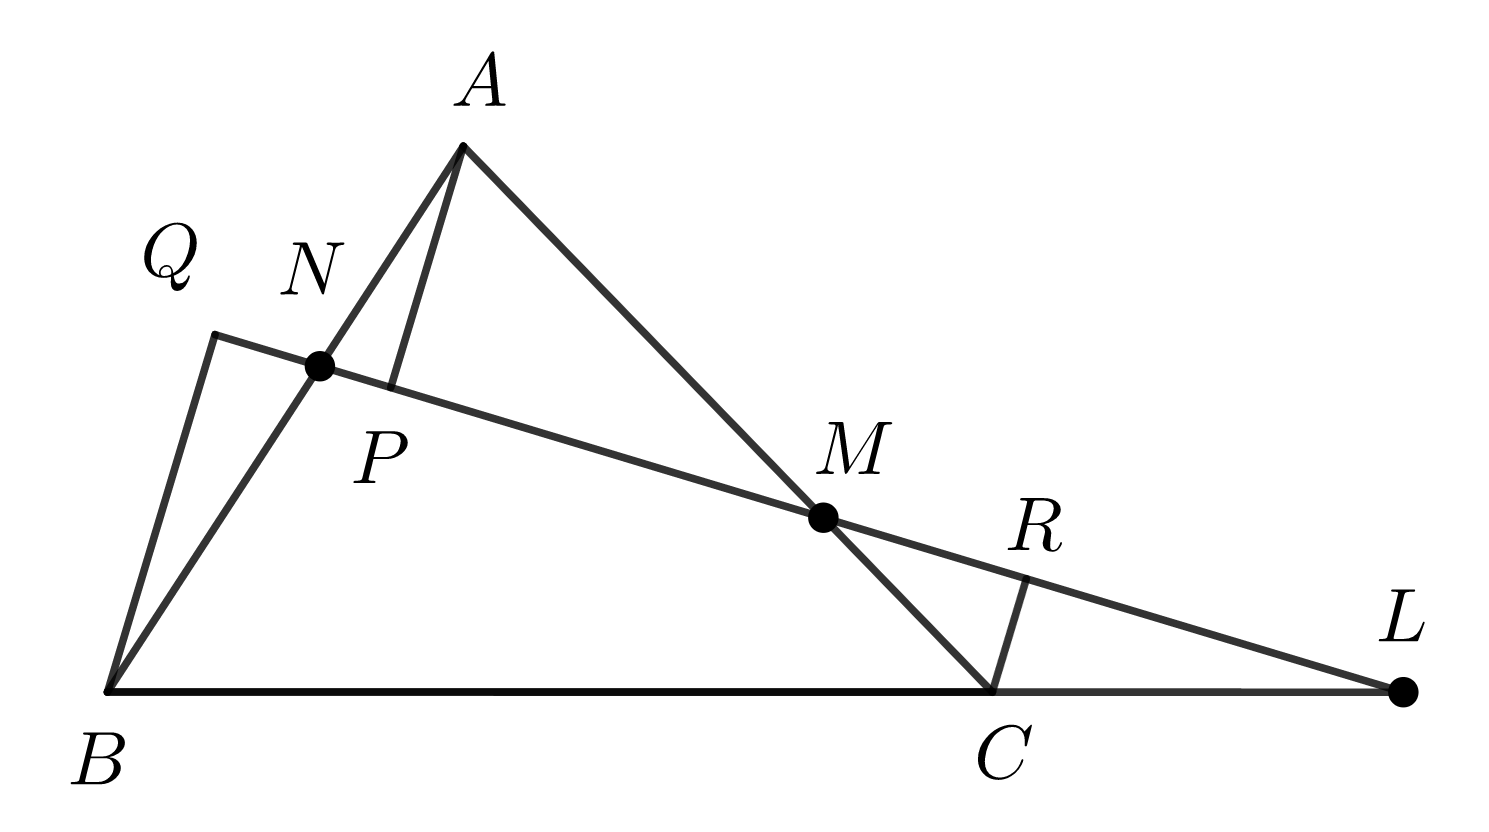
\includegraphics[scale=0.7]{Menelao1.png} 
\end{center}
\subsection*{Demostración:}
\begin{tabular}{p{15.9 cm} p{1cm}}
Sean $AP$, $BQ$, $CR$ las perpendiculares desde $A$, $B$ y $C$, respectivamente, a la recta donde se encuentran $L$, $M$ y $N$.
\\Por criterio de semejanzas, los triángulos rectángulos $APN$ y $BQN$ son semejantes así como los triángulos rectángulos $QBL$ y $RCL$. &(1)
\\Por (1), $\dfrac{AN}{BN}=\dfrac{AP}{BQ}$ y $\dfrac{BL}{LC}=\dfrac{QB}{RC}$ &(3)
\\Por criterio de semejanzas, los triángulos rectángulos $APM$ y $CRM$ también son semejantes.&(4)
\\ De modo que $\dfrac{CM}{AM}=\dfrac{CR}{AP}$
\\Por lo tanto
\end{tabular}
\begin{eqnarray*}
\dfrac{AN}{NB}\cdot \dfrac{BL}{LC}\cdot \dfrac{CM}{MA} &=& \left( - \dfrac{AP}{BQ}\right)  \left( -  \dfrac{QB}{RC} \right) \left( - \dfrac{CR}{AP}\right)
\\&=& \left(- \dfrac{AP}{BQ}\right) \left( \dfrac{BQ}{RC}\right) \left(\dfrac{RC}{AP} \right)
\\&=& -1
\end{eqnarray*}
\begin{tabular}{p{15.9 cm} p{1cm}}
La afirmación inversa se demuestra de manera análoga a la del teorema de Ceva.
\end{tabular}
\subsection*{17. Teorema de la bisectriz.}
Sea un triángulo $ABC$, la bisectriz $AL$, donde $L$ es la intersección de la bisectriz con $BC$, del ángulo en $A$ divide al lado opuesto $BC$ de tal forma que
$$\dfrac{BL}{LC}=\dfrac{AB}{CA}$$
\subsection*{Demostración con bisectriz interna:}
\begin{center}
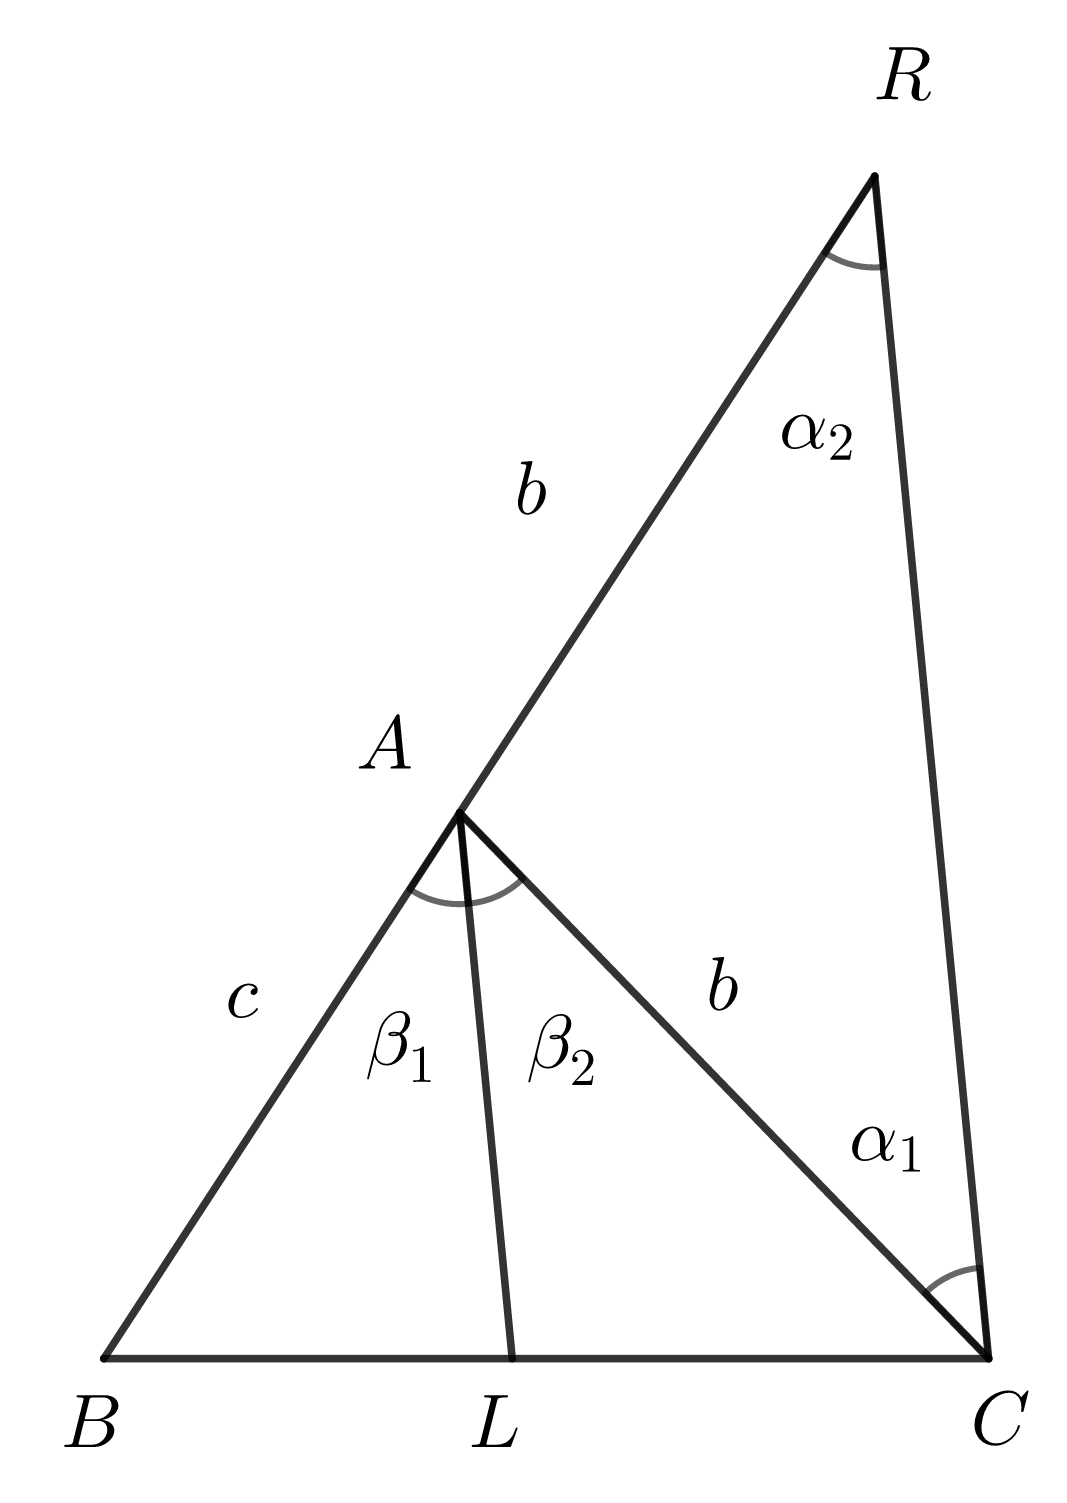
\includegraphics[scale=0.6]{bisectriz_int.png} 
\end{center}
\begin{tabular}{p{15.9 cm} p{1cm}}
Sea $AL$ la bisectriz interna del ángulo interior $BAC$, $b$ y $c$ las longitudes de los lados $CA$ y $AB$, respectivamente. Trazamos a paralela a la bisectriz que pasa por el punto $C$, llamamos $R$ a la intersección de esta recta con la prolongación de $AB$.
\\Por ser rectas paralela y ángulos alternos internos, $\alpha _1= \beta _1$ y $\alpha _2= \beta _2$. &(1)
\\Por hipótesis, $\beta _1= \beta _2$ &(2)
\\Por (1) y (2), $\alpha _1= \alpha _2$&(3)
\\Por (3), el triángulo $ACR$ es isósceles y $AR=b$. &(4)
\\Por ser lados paralelos, los triángulos $RBC$ y $ABL$ son semejantes. (5)
\\Por el teorema de Thales (3), (4) y (5); $\dfrac{BL}{LC} =\dfrac{c}{b}$ como queríamos demostrar
\end{tabular}
\subsection*{Demostración con bisectriz externa:}
\begin{center}
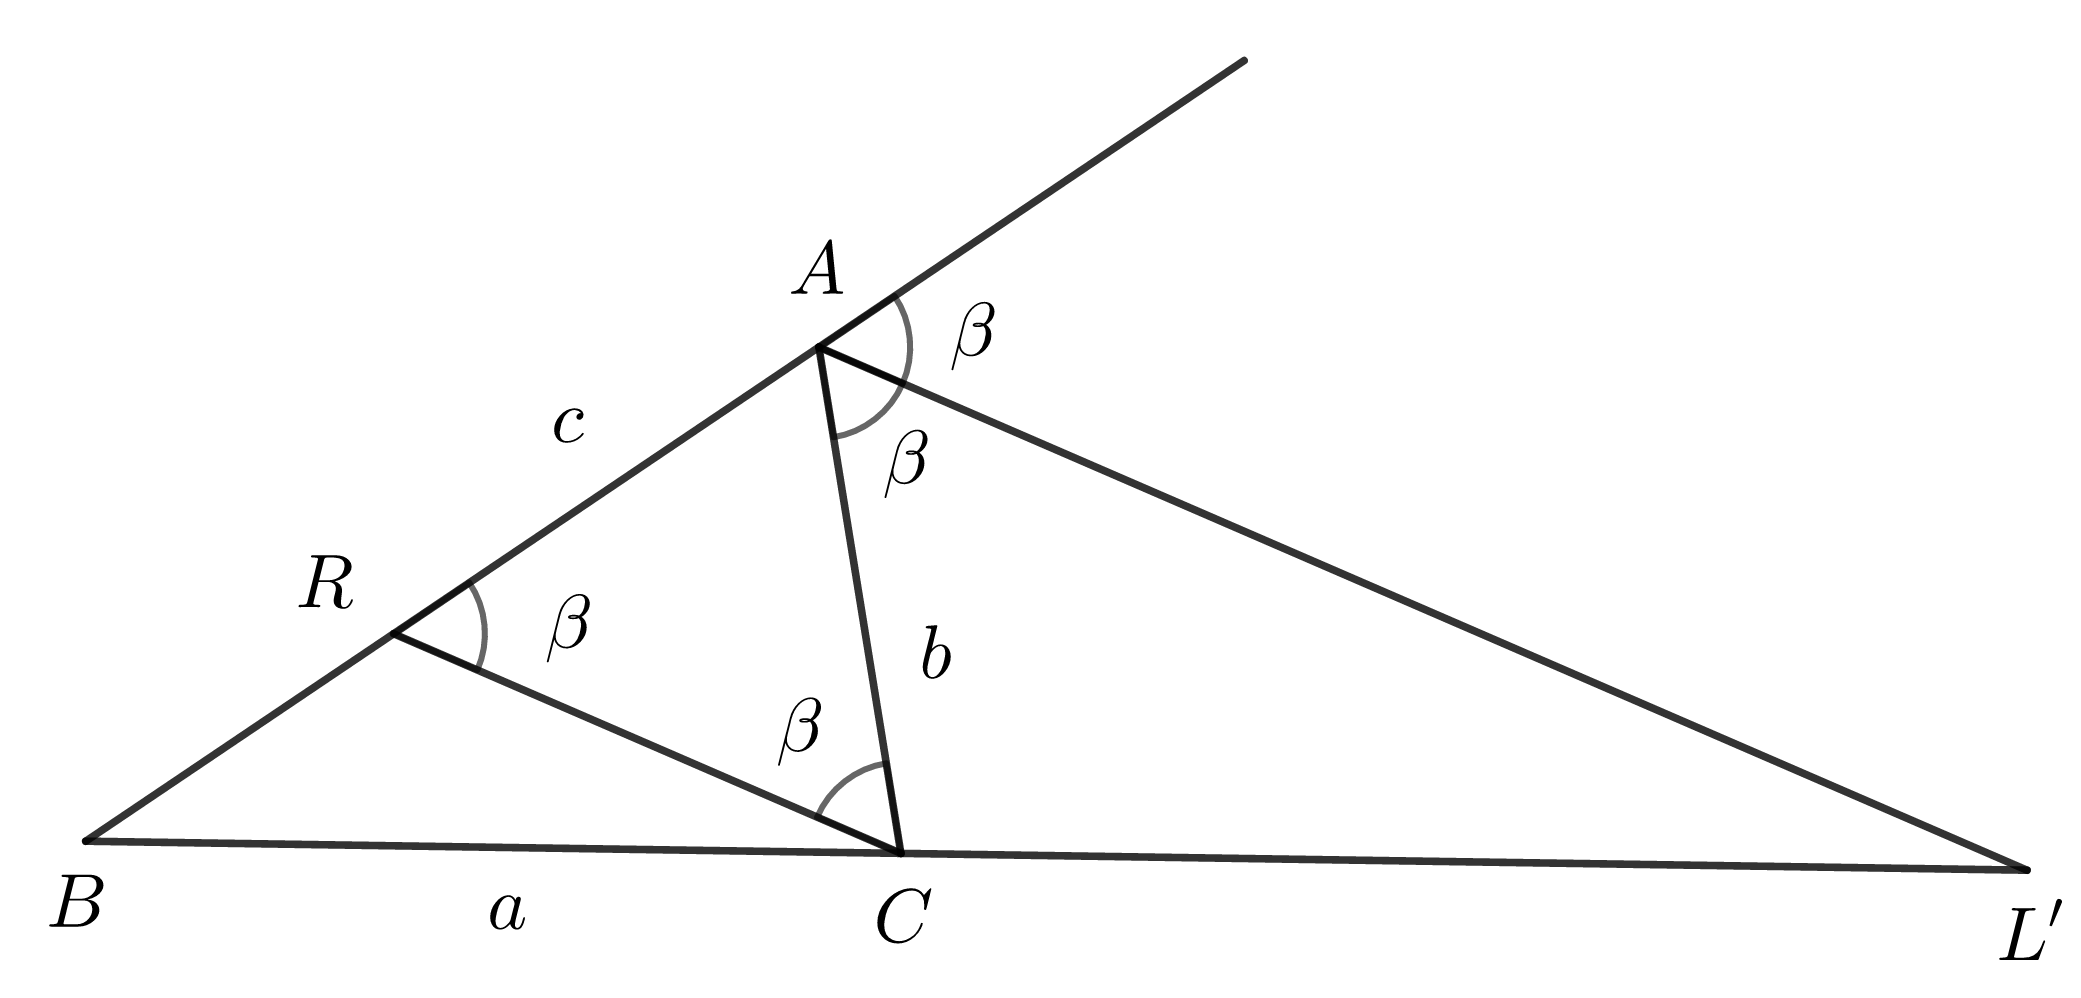
\includegraphics[scale=0.6]{bisectriz_ext.png} 
\end{center}
\begin{tabular}{p{15.9 cm} p{1cm}}
Sea $AL'$ la bisectriz externa del ángulo exterior en $A$ como se muestra en la figura y consideramos $CR$ la recta paralela a $AL'$ que pasa por $C$.
\\Por paralelas y ángulos alternos internos, el triángulo $ARC$ es isósceles. &(1)
\\Por el teorema de Thales y (1), los triángulos $RBC$ y $ABL$ son de lados paralelos, $\dfrac{BL}{LC}=\dfrac{BA}{AR}=\dfrac{c}{b}$
\end{tabular}
\subsection*{18. Teorema de Pappus.}
Si $A$, $C$, $E$ son tres puntos en una recta, $B$, $D$, $F$ tres puntos en otra recta $AB$, $CD$, $EF$ intersectan a las rectas $DE$, $FA$ y $BC$ respectivamente, entonces los tres puntos de intersección $L$, $M$ y $N$ son colineales.
\subsection*{Demostración:}
\begin{center}
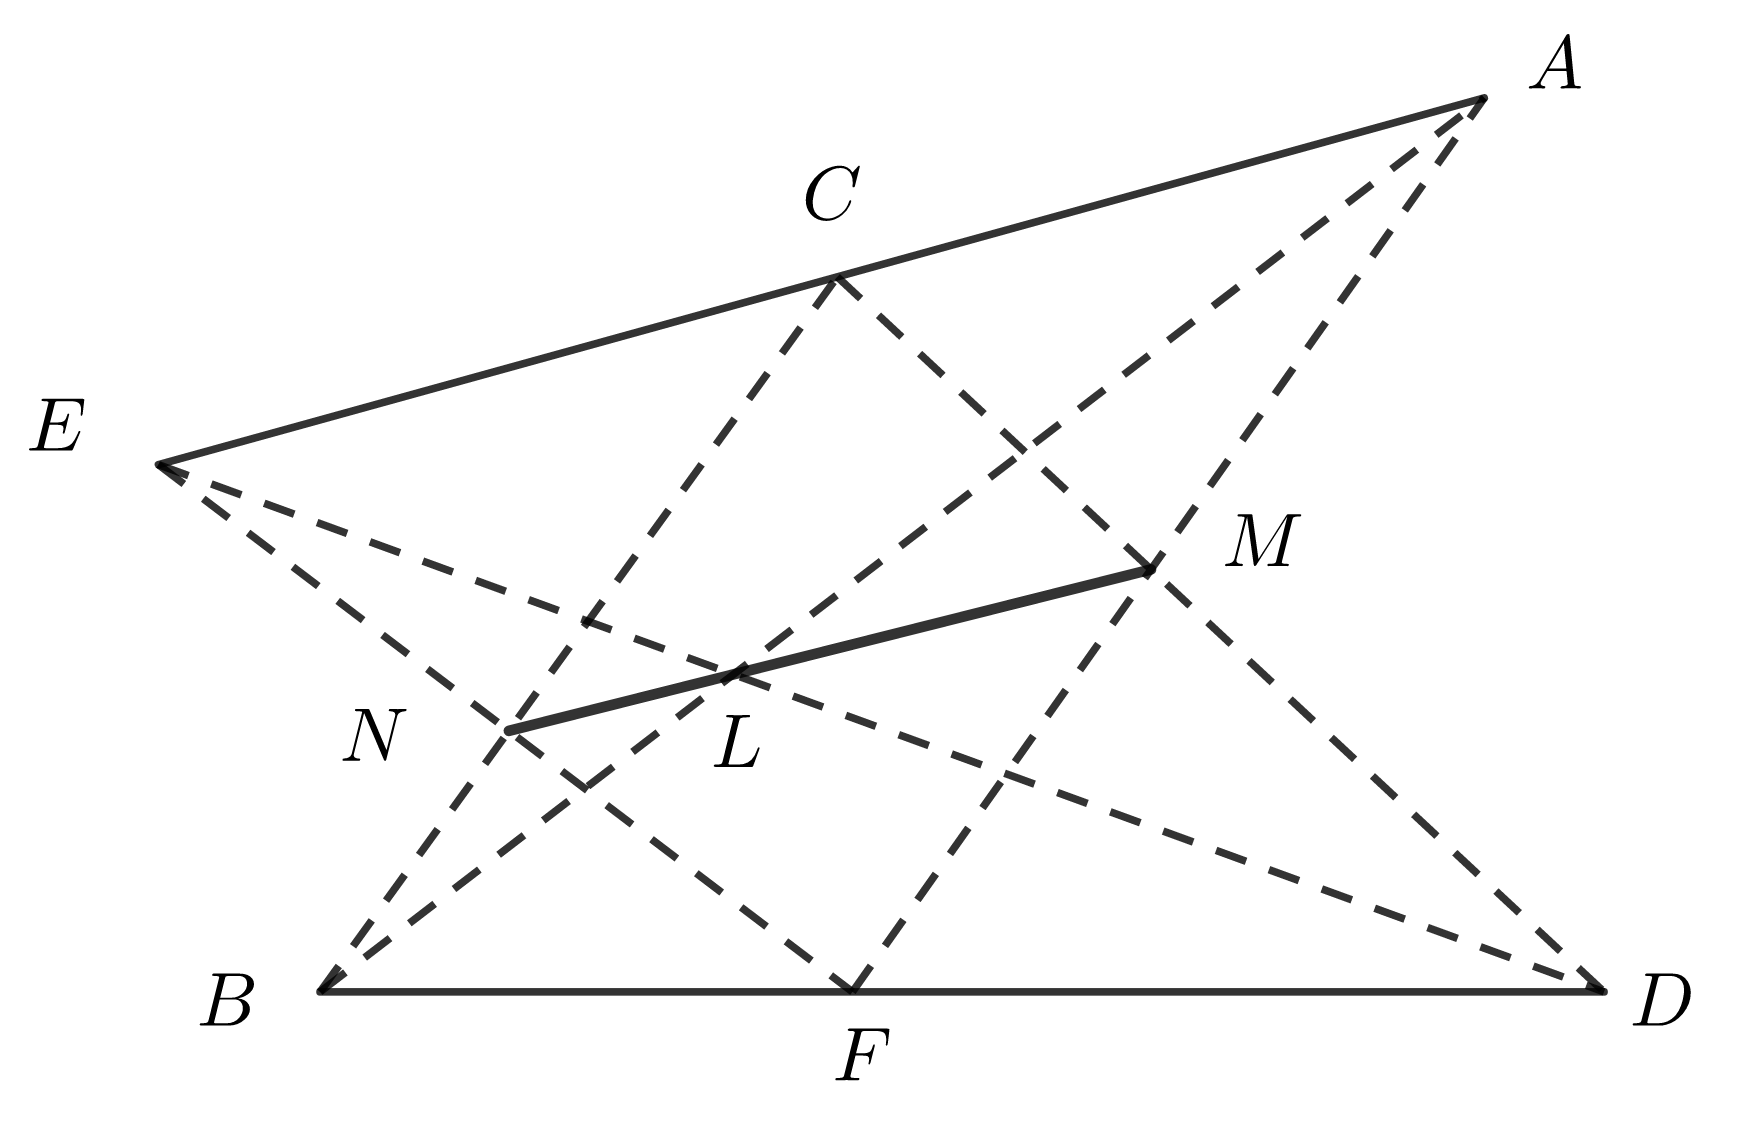
\includegraphics[scale=0.45]{pappus.png} 
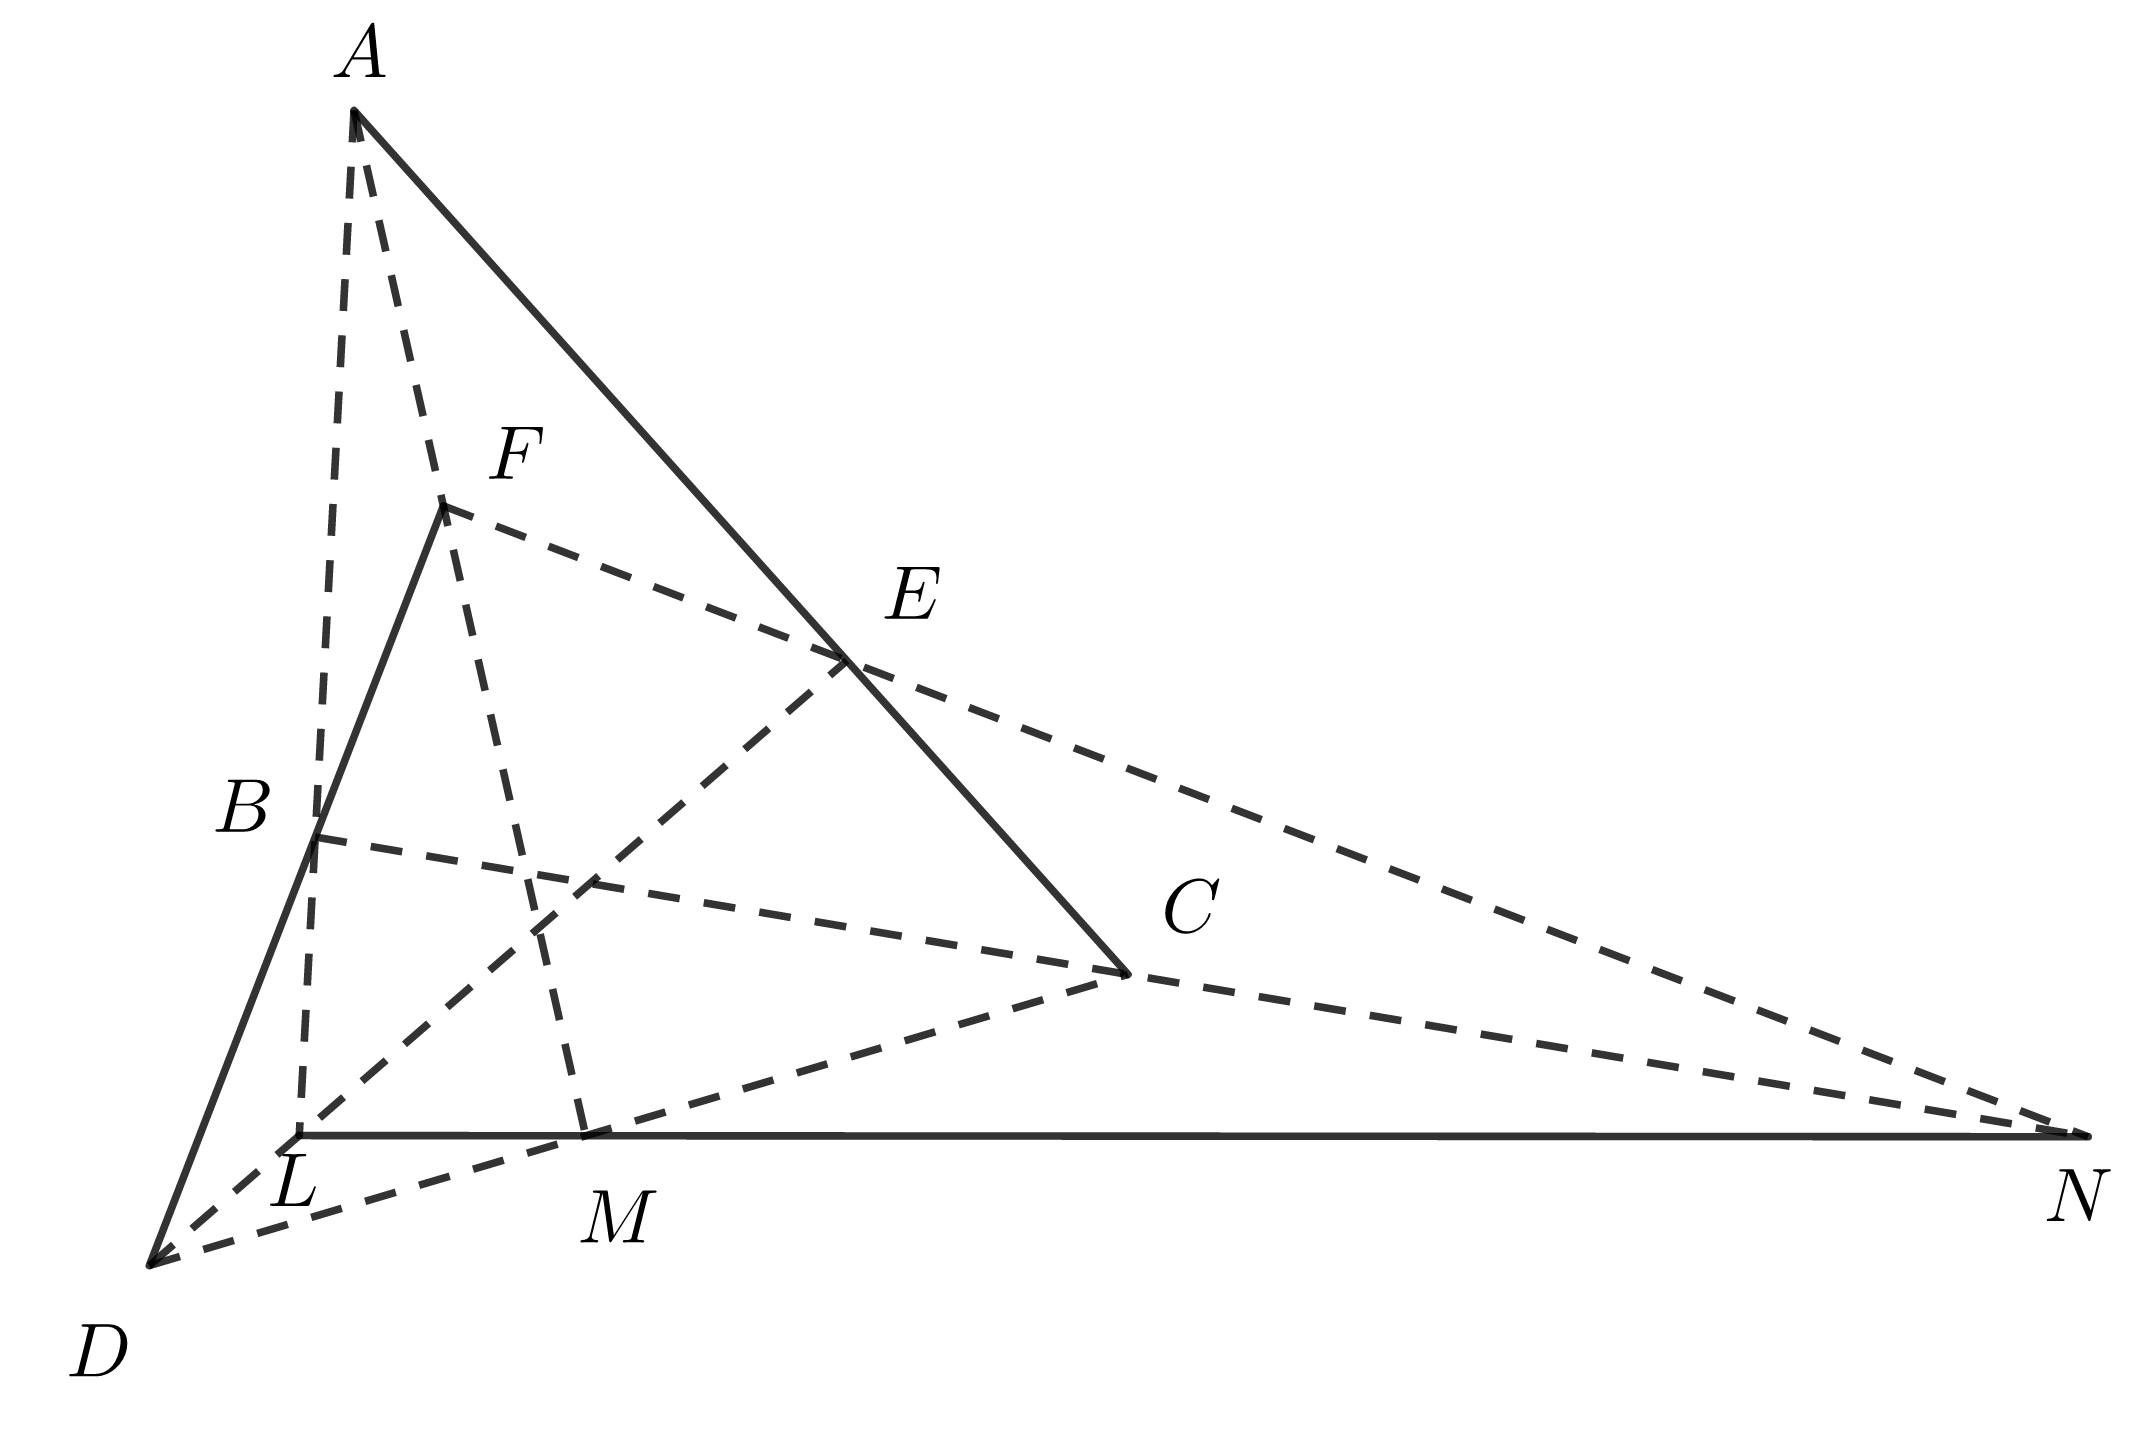
\includegraphics[scale=0.45]{pappus1.png} 
\end{center}
\begin{tabular}{p{15.9 cm} p{1cm}}
\textbf{Observación:} En cada uno de lo conjuntos de tres puntos colineales no importa cual punto está entre los otros dos; de hecho se pueden permutar cíclicamente las letras $A, B, C, D, E$ y $F$ siempre y cuando renombremos también  correctamente las intersecciones. Cualquiera de las siguientes dos figuras cumple las condiciones. para no considerar puntos en el infinito, supondremos que las rectas $AB$, $CD$, $EF$ forman un triángulo $UVW$, como se muestra en la siguiente figura.
\end{tabular}
\begin{center}
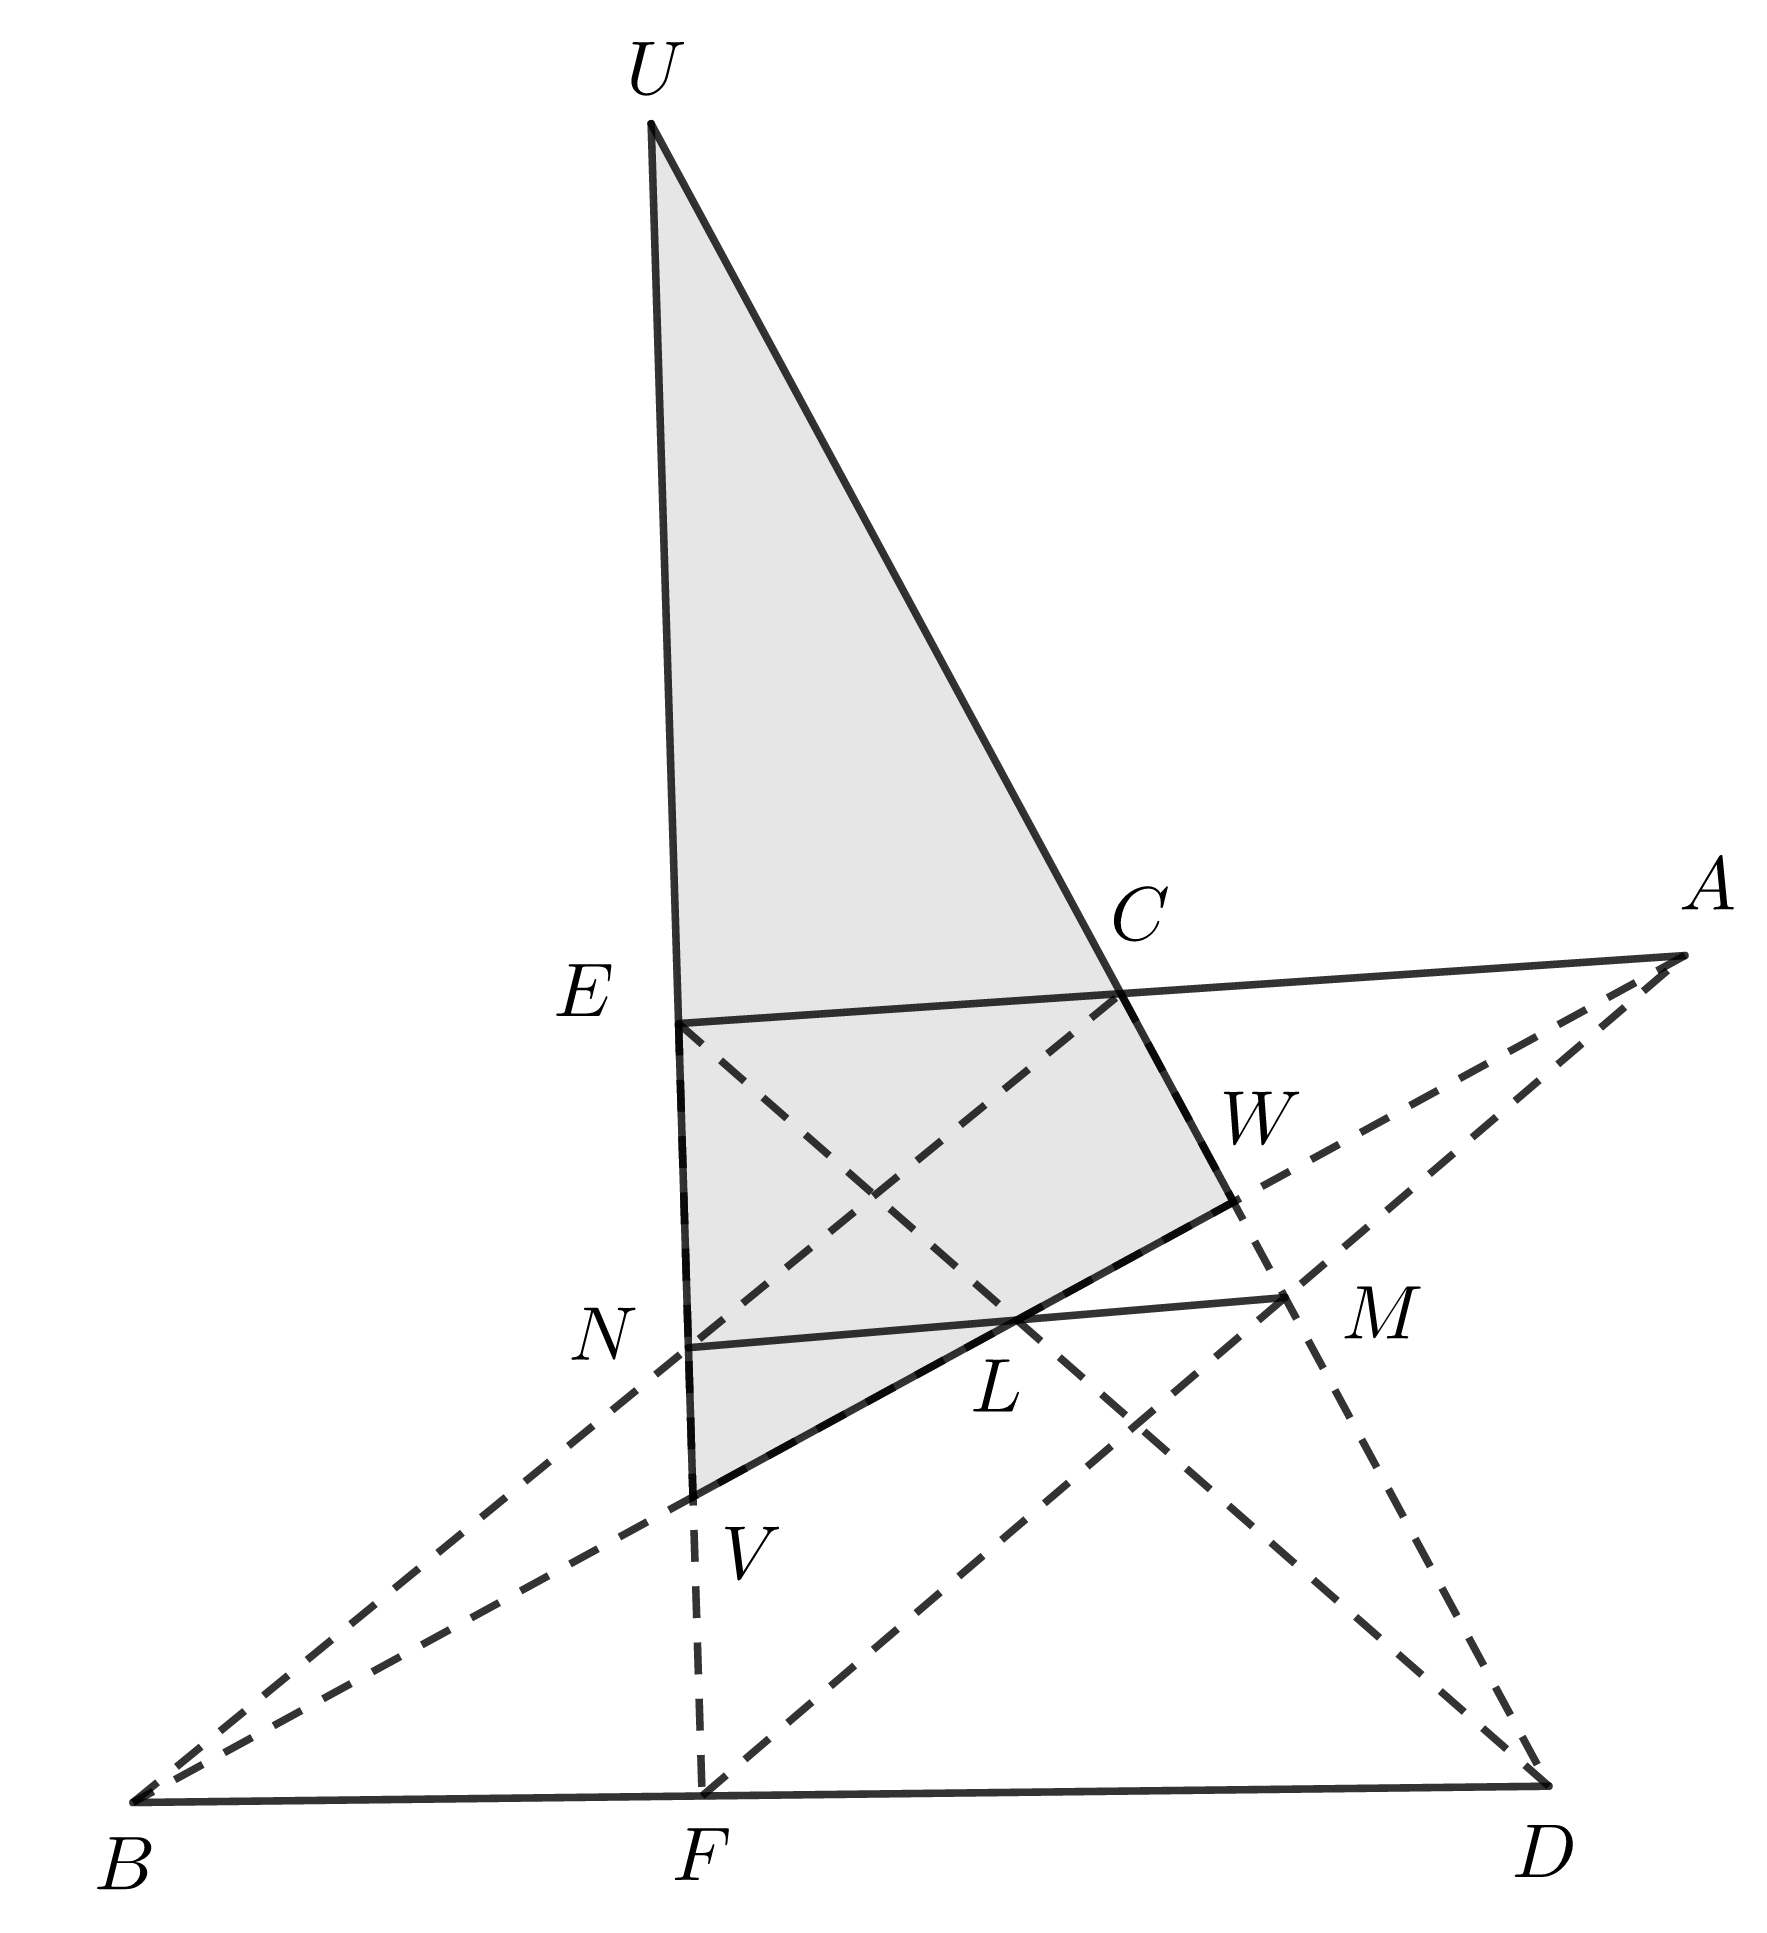
\includegraphics[scale=0.48]{pappus2.png} 
\end{center}
\newpage
\begin{tabular}{p{15.9 cm} p{1cm}}
Por el teorema de Menelao a las ternas de puntos $LDE$, $AMF$, $BCN$, $ACE$, $BDF$ en los lados del triángulo $UVW$ obtenemos:
$$\dfrac{VL}{LW}\cdot \dfrac{WD}{DU}\cdot \dfrac{UE}{EV}=-1,$$
$$\dfrac{VA}{AW}\cdot \dfrac{WM}{MU}\cdot \dfrac{UF}{FV}=-1,$$
$$\dfrac{VB}{BW}\cdot \dfrac{WC}{CU}\cdot \dfrac{UN}{NV}=-1,$$
$$\dfrac{VA}{AW}\cdot \dfrac{WC}{CU}\cdot \dfrac{UE}{EV}=-1,$$
$$\dfrac{VB}{BW}\cdot \dfrac{WD}{DU}\cdot \dfrac{UF}{FV}=-1.$$
Dividiendo el producto de las primeras tres expresiones entre el producto de las últimas dos y cancelando, $\dfrac{VL}{LW} \cdot \dfrac{WM}{MU} \cdot \dfrac{UN}{NV}.$
\\Por lo anterior y el teorema de Menelao, $L$, $M$ y $N$ son colineales como queríamos demostrar.

\end{tabular}
\subsection*{19.1 Teorema de Desargues.}
Si dos triángulos están perspectivas desde un punto y si sus pares de lados correspondientes si intersectan, entonces los tres puntos de intersección son colineales.
\subsection*{Demostración:}
\begin{center}
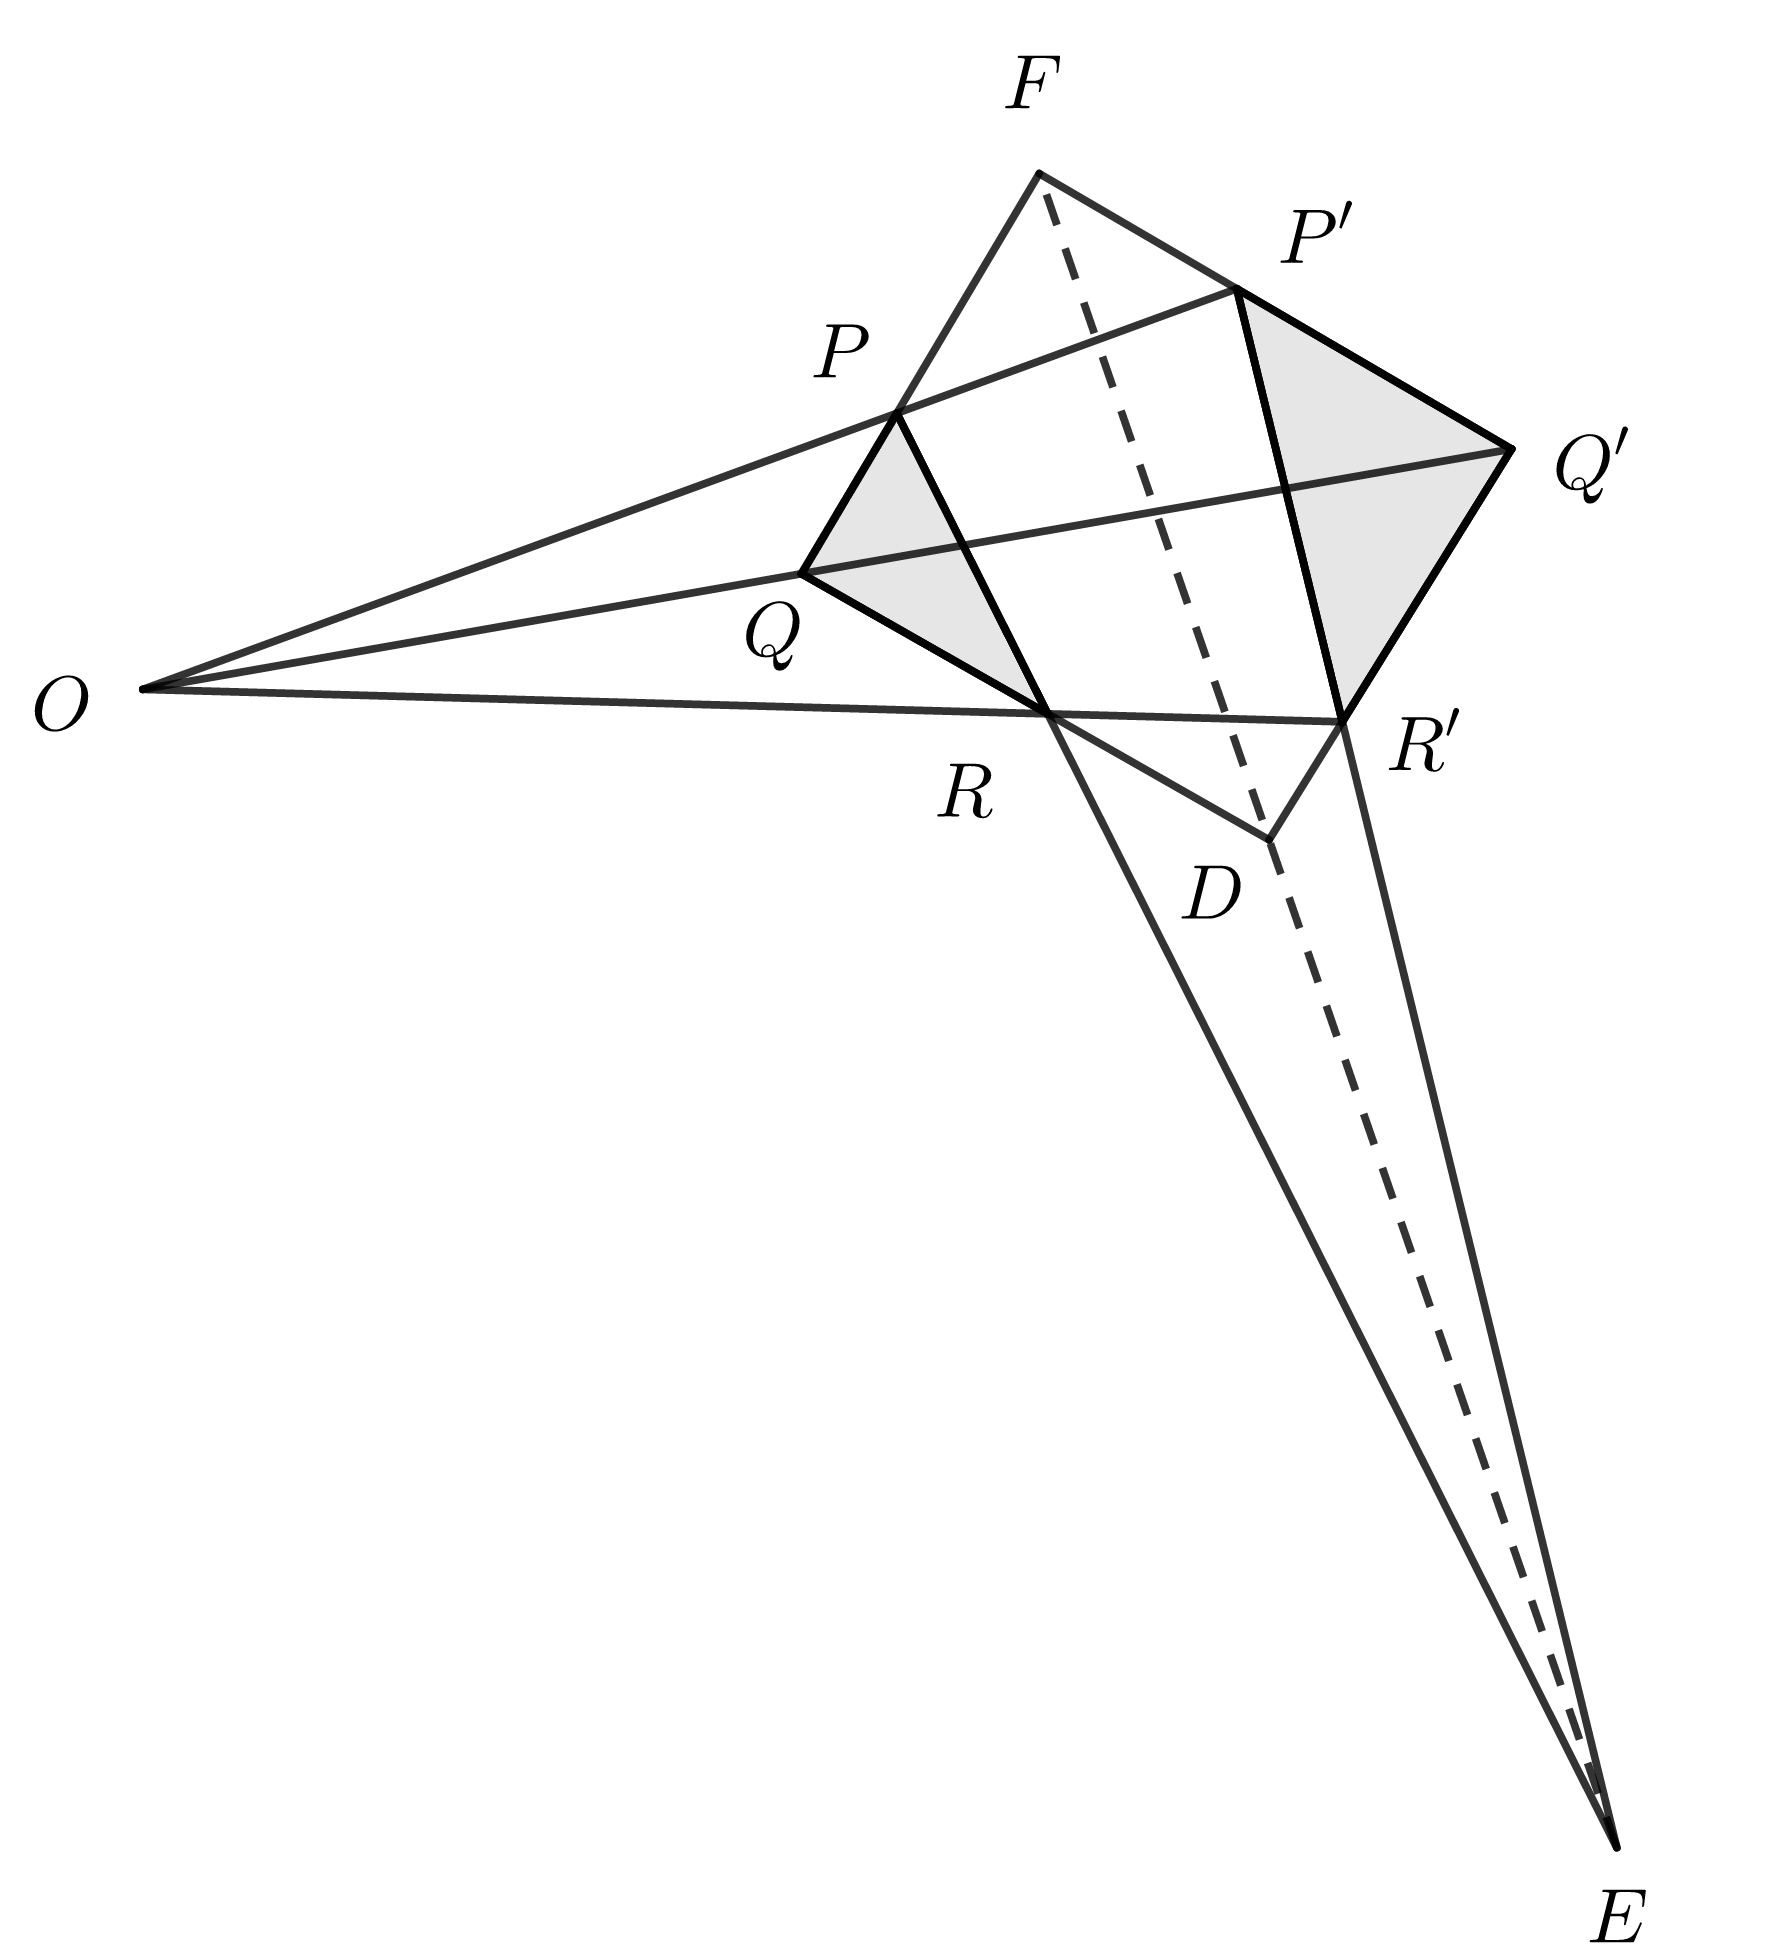
\includegraphics[scale=0.5]{desargue.png} 
\end{center}
\begin{tabular}{p{15.9 cm} p{1cm}}
En la figura los triángulos $PQR$ y $PQR$ están en perspectiva desde $O$ y su pares de lados correspondientes se intersectan en $D$, $E$, $F$ respectivamente.\\Aplicando el teorema de Menelao en las siguientes ternas de puntos, $DR'Q'$, $EP'R'$ y $FQ'P'$, en los lados de los triángulos, $OQR$, $ORP$ y $OPQ$, respectivamente; 
$$\dfrac{QD}{DR}\cdot\dfrac{RR'}{R'O}\cdot\dfrac{OQ'}{Q'Q}=-1,$$ 
$$\dfrac{RE}{EP}\cdot\dfrac{PP'}{P'O}\cdot \dfrac{OR'}{R'R}=-1,$$ $$\dfrac{PF}{FQ}\cdot\dfrac{QQ'}{Q'O}\cdot\dfrac{OP'}{P'P}=-1$$
\\Multiplicando y simplificando respectivamente, considerando los lados dirigidos; $$\dfrac{QD}{DR}\cdot \dfrac{RE}{EP}\cdot \dfrac{PF}{FQ}=-1$$ 
\\Por lo anterior y el teorema de Menelao; $D$, $E$, $F$ son colineales
\end{tabular}
\subsection*{19.2 Teorema.}
Si dos triángulos están están en perspectivas desde una recta, entonces las rectas que unen dos pares de vértices correspondientes son concurrentes; por lo que los triángulos están en perspectiva desde el punto de intersección de estas rectas.
\subsection*{Demostración:}
\begin{tabular}{p{15.9 cm} p{1cm}}
Cuando decimos que los triángulos PQR y P'Q'R' están en perspectiva desde una recta, sabemos que hay tres puntos que son colineales, a saber, los puntos donde se intersectan los lados correspondientes. Llamamos D al punto de intersección de las rectas QR y Q'R', E el punto de intersección de las rectas RP y R'P' y F al punto de intersección de las rectas PQ y P'Q', como se muestra en la figura siguiente.
\\Definimos O como la intersección de las rectas PP' y RR'. Si queremos que QQ' pase por el punto O bastará probar que O es colineal con Q y Q'. Como los triángulos FPP' y DRR' están en perspectiva desde el punto E, aplicamos el teorema directo de Desargues a estos triángulos y concluimos que los puntos de intersección de los lados correspondientes, a saber, O, Q' y Q, son colineales como queríamos.
\end{tabular}
\subsection*{19.3 Teorema.}
Si $PQR$ y $P'Q'R'$ son dos triángulos  en perspectiva desde un punto y éstos tienen dos pares de lados correspondientes paralelos entonces los otros dos lados correspondientes paralelos entonces los otros dos lados correspondientes son paralelos. Recíprocamente, si los triángulos $PQR$ y $P'Q'R'$ tienen lados correspondientes paralelos y dos rectas que unen puntos correspondientes se intersectan en un punto $O$ entonces los triángulos están en perspectiva desde $O$.
\subsection*{20. Teorema.}
El centroide $G$ es el único punto dentro del triángulo $ABC$ que tiene la propiedad de que los triángulos $BCG$, $CAG$ y $ABG$ tienen la misma área.
\subsection*{Demostración:}
\begin{tabular}{p{15.9 cm} p{1cm}}
Sea $A'$, $B'$ y $C'$ los puntos medios de las medianas que van desde $A$, $B$ y $C$, respectivamente. 
\\Sea $M$ un punto en el triángulo $(ABC)$, tal que $(ABM)=(AMC).$
\\Por ser $(ABM)=(AMC)$ y tener los triángulos $ABM$ y $AMC$ a $AM$ como base común, las alturas de $B$ a $AM$ y de $C$ a $AM$ son iguales. 
\\Sea $X$ la intersección de $AM$ con $BC$.
\\Por ser $MX$ común a los triángulos $XMB$ y $XCM$ tener la misma altura sobre las bases $BX$ y $XC$, $BX=XC$. &(1)
\\Por (1), $X$ es punto medio de $BC$. &(2)
\\Por (2), $M$ se encuentra sobre la mediana $AA'$. &(3)
\\EL recíproco se sigue de que $(BA'M)=(A'MC)$ y $(BA'A)=(A'AC)$, donde $A'$ es el punto medio de $BC$.&(4)
\\Por (3) y (4), un punto $M$ dentro del triángulo $ABC$ cumple que $(ABM)=(BCM)=(CAM)$ si y sólo si $M$ se encuentra en las medianas $AA'$, $BB'$ y $CC'$, esto es si sólo si $M$ es el centroide. &\medskip \medskip(5)
\\Consideramos un triángulo $ABC$ y prolonguemos la recta que une los puntos $C'$, $B'$ hasta un punto $A"$ de manera que $A''B'=B'C'=\dfrac{1}{2}BC$.& \medskip (6)
\\Por (6) y paralela media, el cuadrilátero $BA'A''B'$ es un paralelogramo. &(7)
\\Por (7), $A''C=A'B'=\dfrac{1}{2}AB$. &(8)
\\Por (7), (8) y paralela medias, $AC'CA$ es otro paralelogramo &(9)
\\Por (9), $AA''= CC'$. &(10)
\\Por (6) hasta (10), $AA'A''$ es un triángulo donde sus lados $AA'$, $A'A''$, $A''A$ son iguales a las medianas del triángulo $ABC$ &(11)
\\Por paralelas medias, (7) y (9), $A'CA''B'$ es un paralelogramo.
\\Sea el punto de intersección $L$, de las diagonales $B'C$ y $A'A''$.
\\Por (12), $L$ es un punto medio de sus diagonales. &(13)
\\Por (13), $AL$ es mediana del triángulo $AA'A''$. &(14)
\\Análogamente a (14), por ser $AC'A'B'$ paralelogramo, $M$, la intersección de las diagonales $AA'$ y $B'C'$; es punto medio de ellas. &\medskip (15)
\\Por (15), $A''M$ se cortan en $B'$, resulta que $B'$ es el centroide del triángulo $AA'A''$.
\end{tabular} 
\subsection*{21. Teorema.}
El ortocentro de un triángulo acutángulo es el incentro del triángulo órtico.
\subsection*{Demostración:}
\begin{tabular}{p{15.9 cm} p{1cm}}
Veamos algo más sobre las alturas de un triángulo. Consideramos el triángulo ABC, $AD=h_a$ la altura desde el vértice A, O el centro del circuncírculo, y $AA_0$ el diámetro que pasa por A.
\\Los ángulos en B y en $A_0$ son iguales, ya que abren el mismo arco, entonces los triángulos rectángulos ABD y $AA_0C$ son semejantes, por lo que $\dfrac{h_a}{c}=\dfrac{b}{AA_0}$ de donde $h_a=\dfrac{bc}{2R}$
\\Sustrayendo del ángulo BAC los ángulos $A_0AC$ y $BAD$ que son iguales a $90^\circ - \angle B$, tenemos que
$\angle DAA_0 = \angle A -2(90^\circ - \angle B)=\angle A + 2\angle B- (\angle A+ \angle B + \angle C)$
$=\angle - \angle C$
\\Consideramos ahora la extensión de la altura AD hasta que toque al circuncírculo en el punto D'. Tenemos que $\angle DAB = \angle FCB$, ya que ambos son complementarios  del ángulo en B. También $\angle BCD' = \angle BAD'$, por abrir  el mismo arco, luego los triángulos rectángulos CDH y CDD' son congruentes y nos muestran que HD= DD'
\end{tabular}
\subsection*{22. Teorema.}
Las bisectrices externas de cualesquiera dos ángulos de un triángulo son concurrentes con la bisectriz interna del tercer triángulo son concurrentes con la bisectriz interna del tercer ángulo.
\subsection*{23. Teorema.}
Sea $\alpha$ y $\beta$ dos ángulos cualesquiera, se cumple que:$$\cos ( \alpha \pm \beta) = \cos \alpha \cos \alpha \mp \sin \alpha \sin \beta$$
$$\sin (\alpha \pm \beta) = \cos \alpha \sin \beta \pm \cos \beta \sin \alpha$$
\subsection*{Demostración:}
\begin{tabular}{p{15.9 cm} p{1cm}}
Sea $AD$ un segmento perpendicular a $OB$ como se muestra en la figura. Consideramos el triángulo rectángulo $OAD$ y el segmento $AC$ perpendicular a la recta $OE$.
\\Definimos $\alpha$ y $\beta$ como $\angle COA$ y $\angle BOC$, respectivamente
\\Por definición de coseno e hipótesis, $cos(\alpha + \beta) = \dfrac{OD}{OA}=\dfrac{OB-OD}{OA}=\dfrac{OB-CF}{OA}$ &(1)
\\Por definición de coseno e hipótesis,
$cos \beta = \dfrac{OC}{OA}, cos \alpha = \dfrac{OB}{OC}$ &(2)
\\Por definición de seno e hipótesis, $sen \beta = \dfrac{AC}{OA}$ &(3)
\\Por ambos estar formado por el rayo $OE$ y ser la recta $l$ paralela a $FH$ por construcción, $\angle ECH$ y $\alpha$ son iguales. &\medskip(4)
\\Por (4) y ser $AC$ perpendicular a $OE$, los triángulos $OGD$ y $AGC$ son semejantes &(5)
\\Por (5), $\alpha =\angle GAC$ &(6)
\\Por (6), $\alpha + \angle ACF= 90^{\circ}$  &(7)
\\Por (6) y (7), $\cos \angle ACF = \sen \alpha$&(8)
\\Por (1), (2), (3) y (8); $\cos \angle ACF = \dfrac{CF}{AC}$ &(9)
\\Por (8) y (9), $CF= AC \cos \angle ACF= AC \sen \alpha$
\\Sustituyendo respectivamente, $ \cos( \alpha + \beta)=\dfrac{OC \cos \alpha - AC \sen \alpha}{OA}$ $=\cos \beta \cos \alpha - \sen \beta \sen \alpha$ &(10)
\\Análogo a (10), $\cos (\alpha + \beta)= \cos \beta \cos \alpha + \sen \beta \sen \alpha $ &(11)
\\Análogo a (10), $\sin (\alpha \pm \beta) = \cos \alpha \sin \beta \pm \cos \beta \sin \alpha$
\end{tabular}
\subsection*{24. Teorema.}
Sea $\alpha$ un ángulo cualquiera,$$\cos^ 2 \alpha + \sin ^2 \alpha =1$$
\subsection*{25. Teorema de los cosenos.}
Sea un triángulo con $a$, $b$ y $c$ las longitudes de los lados y $\beta$ el ángulo opuesto al lado $b$.
$$b^2 = a^2 + c^2 =2ac \cos \beta$$
\subsection*{Demostración:}
\begin{tabular}{p{15.9 cm} p{1cm}}
Trazamos la altura desde el vértice $A$ y llamamos $D$ al pie de la altura. Definimos $x=BD$.
\\Por definición, $DC=a-x.$ &(1)
\\Por (1) y el teorema de Pitágoras aplicado a los triángulos $ADC$ y $ABD$, $b^2=(a-x)^2 + h^2$ y $c^2=x^2 +h^2$.  respectivamente. & \medskip (2)
\\Por (2), $b^2=a^2-2ax+x^2+h^2$ y $b^2=a^2- 2ax+c^2$. &(3)
\\Por definición de coseno e hipótesis, $cos\beta = \dfrac{x}{c}$  &(4)
\\Por (3) y (4) , $b^2= a^2 +c^2-2ac cos \beta$
\end{tabular}
\subsection*{26. Ley de los senos.}
Sea $ABC$ un triángulo inscrito en una circunferencia de radio $R$. Si $a$, $b$ y $c$ son los lados del triángulo opuestos a los vértices $A$, $B$ y $C$ respectivamente, entonces$$ \dfrac{a}{\sin A} = \dfrac{b}{\sin B}= \dfrac{c}{\sin C}= 2R$$
\subsection*{Demostración:}
\begin{tabular}{p{15.9 cm} p{1cm}}
Consideramos el triángulo $ABC$ y su circuncírculo de radio $R$. Dibujamos el diámetro $CJ$ y la cuerda $BJ$.
\\Por ser $CJ$ diámetro, $\angle CBJ$ es un ángulo recto. &(1)
\\Por subtender de la misma cuerda hacia el mismo  semiplano, $ \angle BJC= \angle BAC$ &(2)
\\Por (1) y (2), $sen \angle BAC = sen \angle BJC = \dfrac{a}{CJ}=\dfrac{a}{2R}$ &(3)
\\ Por (3), $\dfrac{a}{\sen A} = 2R$
\\Considerando el caso en que $\angle A$ es no obtuso, \\Consideramos la siguiente figura donde hemos trazado el diámetro $CJ$.
\\Por ser los ángulos opuestos en un cuadrilátero cíclico, $\angle BJC = 180^{\circ} - \angle BAC$. &(4)
\\Por propiedades de senos, $sen \theta = sen (180^{\circ}-\theta)$ &(5)
\\Por (4) y (5), $sen \angle BJC = sen \angle BAC$. &(6)
\\Por (6), $sen A= sen \angle BAC = sen \angle BJC = \dfrac{a}{2R}$
\end{tabular}
\subsection*{27. Teorema de Stewart.}
Sean $ABC$ un triángulo y $AX$ una ceviana de longitud $p$, que divide al segmento $BC$ en dos segmentos $BX=m$ y $XC=n$; $$a(p^2 +mn) = b^2m + c^2m$$
\begin{center}
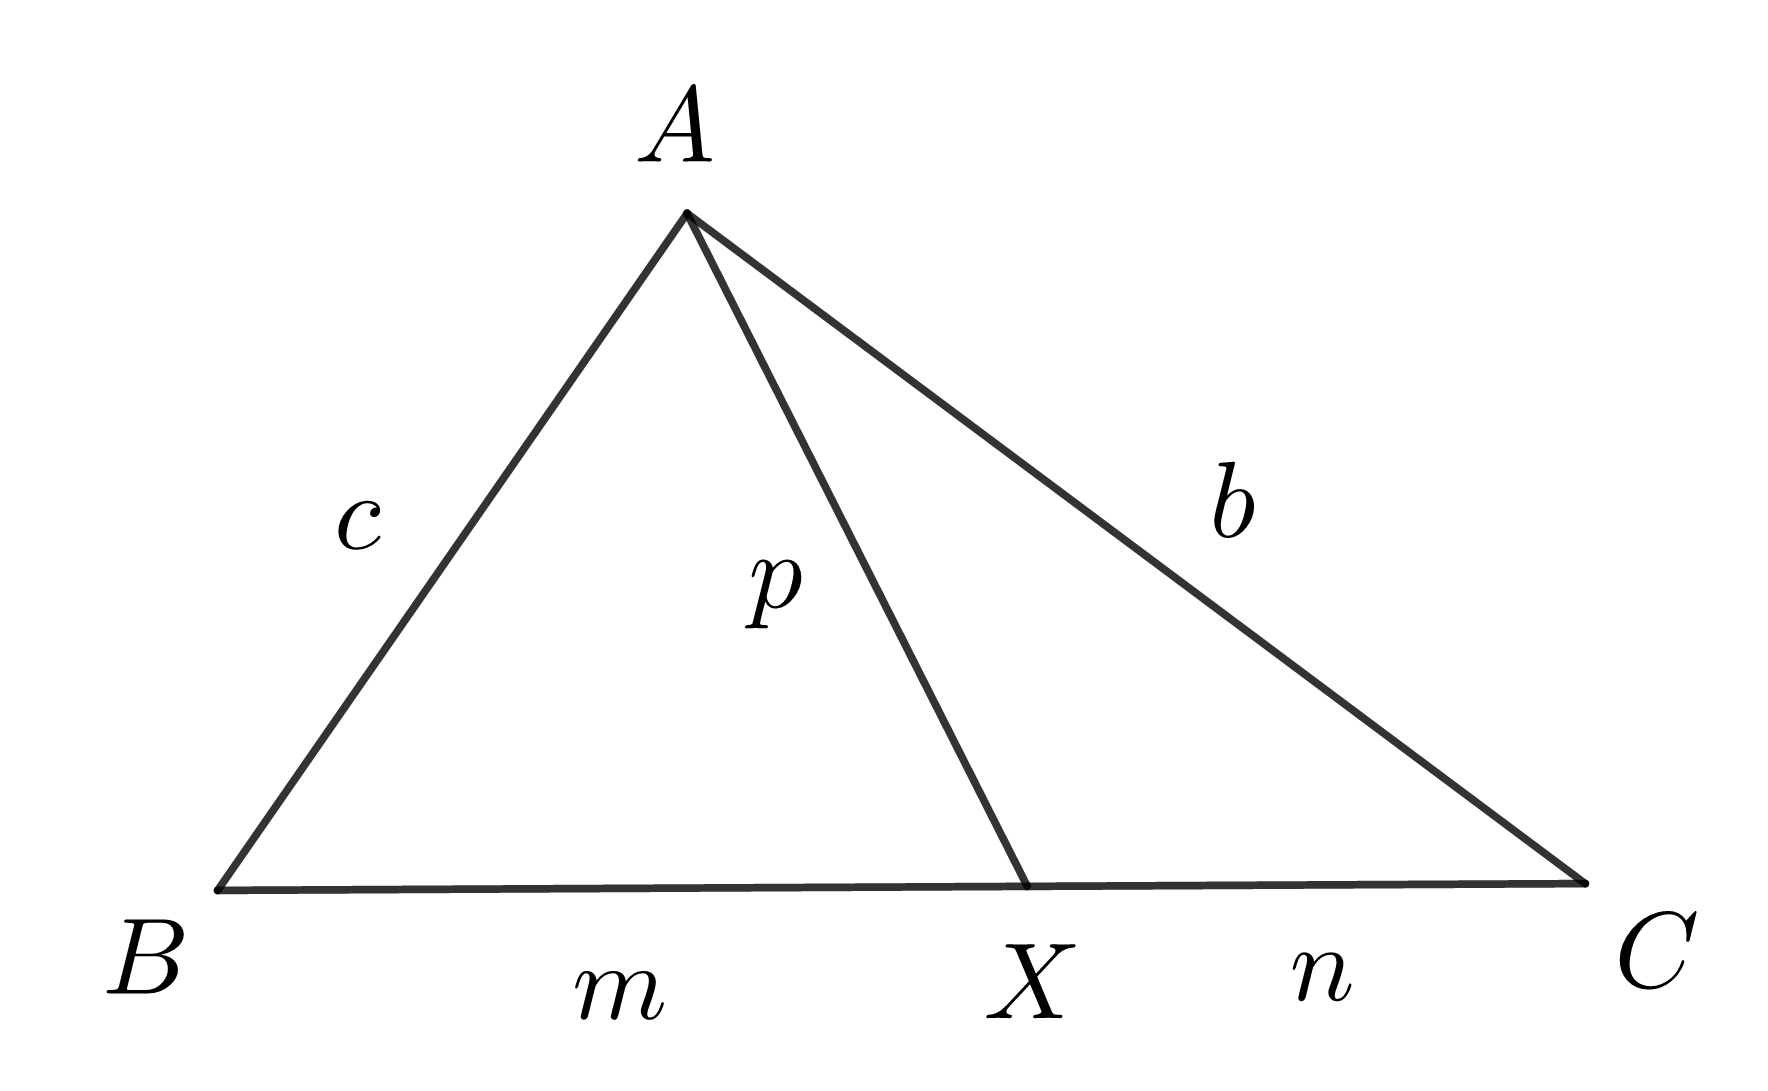
\includegraphics[scale=0.6]{stewart.png} 
\end{center}
\subsection*{Demostración:}
Definimos $\theta=\angle CXA$.
\\Por la ley de los cosenos aplicada en los ángulos suplementarios en $X$,
\setcounter{equation}{0}
\begin{align}
b^2&= p^2 + n^2-2pn \cos \theta,\\
c^2&= p^2 + m^2-2p \cos (180^{\circ}-\theta)
\end{align}
Multiplicando (1) por $m$, (2) por $n$, y sumando término a término, 
\begin{eqnarray}
b^2m + c^2n=\ p^2(m+n)+mn(m+n)-2mnp(cos(180^{\circ}-\theta)+cos \theta )
\end{eqnarray}
Por (3), propiedades de cosenos y ser $m+n=a$;
$$b^2m + c^2n=a(p^2+mn)$$
\subsection*{28. Fórmulas de área de un triángulo.}
Sea $ABC$ un triángulo con lados de longitud $a$, $b$, y $c$. Si $s$, $r$ y $R$ son el semiperímetro, el inradio y el circunradio del triángulo, respectivamente: Entonces su área las podemos calcular como:
\begin{eqnarray*}
(ABC)&=& \dfrac{ac \sin \angle CBA}{2}
\\&=& \dfrac{abc}{4R}
\\&=& sr
\\&=& \sqrt{s(s-a)(s-b)(s-c)}
\end{eqnarray*}
\subsection*{Demostración:}
1. Trazamos la altura sobre la BC desde el vértice A, tenemos dos casos: el pie de la altura D, se encuentra a la derecha de B o a la izquierda de B. En el primer casa $h_a= c sen \angle CBA$ y en el segundo caso $h_a= c sen \angle ABD$; pero como; pero $\angle CBA$ y $\angle ABD$ son ángulos sumplemetarios, tenemos que: $sen \angle CBA= sen \angle ABD,$ luego en cualquier caso $h_a=c sen \angle CBA$.
\\Ahora de 
esta última igualdad y del hecho que $(ABC)= \dfrac{a h_a}{2}$ tenemos que $(ABC)=\dfrac{ac sen \angle CBA}{2}$
2. El área del triángulo ABC es $(ABC)=\dfrac{ah_a}{2}$, al sustituir el valor de $h_a$. dado en la ecuación, tenemos que: $(ABC)=\dfrac{abc}{4R}$
\\3. Consideramos i el incentro del triángulo ABC y fijémonos en los striángulos ABI, BCI y CAI. El área del triángulo ABC es igual a la suna (ABI) + (BCI) y (CAI). Las áreas de cada uno de lo striángulos están dadas por $(ABI)= \dfrac{AB r}{2}= \dfrac{cr}{2}$, $(BCI)=\dfrac{ar}{2}$, $(CAI)=\dfrac{br}{2}$, donde r es el radio del incírculo, entonces:
$(ABC)=\dfrac{cr}{2}+\dfrac{ar}{2}+\dfrac{br}{2}=\dfrac{ar+br+cr}{2}=\dfrac{(a+b+c)}{2}=sr$
\\4.La ecuación de la nos dice que
$r=\sqrt{\dfrac{(s-a)(s-b)(s-c)}{s}}$
\\luego, multiplicando por $s$ tenemos
$ rs=\sqrt{s(s-a)(s-b)(s-c)}$
\subsection*{29. Desigualdad geométrica.}
Si $a$, $b$, $c$ son los lados de un triángulo de área $(ABC)$ entonces $$4\sqrt{3}(ABC) \leq a^2 + b^2 + c^2$$
\\con igualdad si y sólo si $a$, $b$, $c$ es equilátero.
\subsection*{Demostración:}
Como un tri;angulo equilátero de lado $a$ tiene área igual a $\dfrac{\sqrt{3}}{4}a^2$, la igualdad se alcanza en tal caso. Trataremos de comparar lo que sucede en un triángulo cualquiera respecto a lo que  pasa en  un triángulo equilátero de lado $a$. 
\\Si AD es el altura del triángulo desde A, su longitud la podemos escribir de la forma $h=\dfrac{\sqrt{3}}{2}a+y$, donde $y$ y mide su defecto con respecto a la altura del triángulo equilátero. También escribimos $BD=d=\dfrac{a}{2}-x$ y $DC=e=\dfrac{a}{2}+x$, donde $x$ se puede interpretar  como el defecto que tiene el pie de la altura con respectivo al pie de la altura en el caso equilátero ( que en caso es el punto medio del lado BC). Tenemos que:
\begin{eqnarray*}
a^2+ b^2+ c^2 -4\sqrt{3}(ABC) &=& a^2 + h^2 +(\dfrac{a}{2}+x)^2 + h^2+(\dfrac{a}{2}-x)^2- 4\sqrt{3}\dfrac{ah}{2}
\\&=& \dfrac{3}{2}a^2 +2h^2 + 2x^2 -2\sqrt{3}a(\dfrac{\sqrt{3}}{2}a+y)
\\&=&\dfrac{3}{2}a^2 + 2\dfrac{\sqrt{3}}{2}a+y)^2 +2x^2-3a^2-2\sqrt{3}ay
\\&=& \dfrac{3}{2}a^2 + \dfrac{3}{2}a^2 +2\sqrt{3}ay +2y^2+ 2x^2-3a^2- 2\sqrt{3}ay
\\&=&2(x^2+y^2)\geq 0
\end{eqnarray*}
Además la igualdad se da si y sólo si x=y=0 y sólo si el triángulo es equilátero
\subsection*{30. Desigualdad de Nesbitt.}
Sea $a$, $b$ y $c$ números positivos, se cumple que:
$$\dfrac{a}{b+c} + \dfrac{b}{c+a}+ \dfrac{c}{a+b} \geq \dfrac{3}{2}$$
\subsection*{Demostración:}
\begin{eqnarray*}
\dfrac{a}{b+c}+ \dfrac{b}{c+a}+\dfrac{c}{a+b}&=&
\dfrac{a+b+c}{b+c}+\dfrac{a+b+c}{c+a}+\dfrac{a+b+c}{a+b}-3
\\&=&(a+b+c)\left(\dfrac{1}{b+c}+\dfrac{1}{c+a}+\dfrac{1}{a+b}\right)-3
\\&=&\dfrac{1}{2}[(a+b)+(b+c)+(c+a)]\left(\dfrac{1}{b+c}+\dfrac{1}{c+a}+\dfrac{1}{a+b}\right)-3
\\&\geq&\dfrac{9}{2}-3=\dfrac{3}{2}
\end{eqnarray*}
\subsection*{31.1 Transformación de Ravi.}
Sea $a$, $b$ y $c$ lados del triángulo, entonces $a=x+y, b=y+z, c=z+x$ con $x$, $y$, $z$ pertenecientes a los reales positivos.
\subsection*{Demostración:}
Mostramos el incírculo del triágnulo ABC que, su centro es el punto de concurrencia de las bisectrices. LLamamos X, Y, Z los puntos,  de tangencia con el lado BC, CA y AB, respectivamente.
\\ Como las dos tangentes desde cualquier punto exterior a una circunferencia son iguales,, tenemos que Ay=AZ=x, BZ= BX=y, CX=CY=z. Entonces. y+z=a, z+x=b,  x+y =c
\subsection*{31.2 Teorema.}
Sea $a$, $b$ y $c$ lados del triángulo, con $a=x+y, b=y+z, c=z+x$, entonces:
$$i) x+y+z=s$$
$$ii) x=s-a , y=s-b, z=s-c$$
\subsection*{Demostración:}
\subsection*{32. Desigualdad geométrica.}
Sean $A$, $B$ y $C$ ángulos de un triángulo, $$\cos A =\cos B +\cos C \leq \dfrac{3}{2}$$ 
\subsection*{Demostración:}

\subsection*{33.1. Teorema de Potencia de punto.}
Si las cuerdas $AB$ y $CD$ son cuerdas; $A, B, C, D$ están sobre una misma circunferencia, si y sólo si intersectan en un punto $P$ y cumple que $$PA \cdot PB = PC \cdot PD$$
\subsection*{Demostración:}
Si el punto de intesección se encuentra sobre la circunferencia, ambos miembros de la ecuación son cero y la igualdad es inmediata. Supongamos que P se encuentra en el interior de la circunferncia. Los triángulos PAD y PCB son semejantes ya que los ángulos $\angle PAD$ y $\angle PCE$ son iguales por abrir el mismo arco, de igual manera por abrir el mismo arco los ángulos $\angle PDA$ y $\angle PBC$ son iguales. Por tanto $\dfrac{PA}{PC}=\dfrac{PD}{PB}$ y entonces: $PA \cdot PB = PC \cdot PD$
\\Si P se encuentra fuera de la circunferencia tenemos, por ser el cuadrilátero PAC y PDB son semejantes y $PA \cdot PB= PC \cdot PD$
\subsection*{33.2. Teorema del Centro Radical.}
Los ejes radicales de tres circunferencias se intersectan en un punto $P$.
\subsection*{34.Teorema de Fórmula de Euler.}
Una condición necesaria y suficiente para la existencia de un triángulo con circuncírculo $( O, R)$ e incírculo $(I, r)$ es la igualdad $$OI ^2= R^2 - 2Rr$$
\subsection*{Demostración:}
Sea A un punto sobre el circuncírculo C=(O, R), Sean B y C los puntos de intersección del circuncírculo C con las tangentes desde A al círculo C'=(I, r). El triángulo admite a C' como incírculo si y sólo si BC es tangente a C', si y sólo si $\angle ABI= \angle IBC$
\\Sea D el punto de intersección de la recta AI con círculo C. Como AI es bisectriz, tenemos que $\angle IAB= \angle CAI$. Además $\angle CAI= \angle CBD$, ya que ambos ángulos abren el mismo arco CD, luego $\angle IAB= \angle CBD$. Como el ángulo $\angle BID$ es ángulo exterior del triángulo ABI, tenemos que $\angle IAB= \angle BID =- \angle ABI$. Además como $\angle CBD = \angle IBD - \angle IBC$, y $angle IAB= \angle CBD$ obtenemos que $\angle BID - \angle ABI= \angle IBD - \angle IBC$. Luego la condición $\angle ABI = \angle IBC$ es verdadera si y sólo si $\angle BID = \angle IBD$. Pero estos dos ángulos, son los ángulos opuestos a los lados BD y ID dle triángulo IBD.
\\Podemos reformular el rpoblema como sigue: El triángulo ABC admite a C'=(I, r) como incírculo si y sólo si BD=ID.
\\Sea E el punto de tangencia del círculo C' con Ab y D' el punto diametralmente opuesto a D en C. Como los triángulos rectángulos AIE  y D'DB tienen los ángulos IAE y DD'B iguales  por abrir el mismo arco BD, resulta que son semejantes. Esta semejanza nos garantiza que $\dfrac{AI}{IE}= \dfrac{D'D}{DB}$, por lo que: $AI \cdot DB= 2Rr$
\\ AL tomar la potencia del punto I con respecto al círculo C, tenemos: $AI \cdot ID =(R-d)(R+d) $, donde $d=OI$. De las dos últimas igualdades obtenemos:
$\dfrac{DB}{ID}=\dfrac{2Rr}{(R-d)(R+d)}=\dfrac{2Rr}{(R^2-d^2)}$
\\Luego, BD=ID si y sólo si $ R^2- d^2=2Rr$
\subsection*{35. Teorema de Homotecia.}
Dos circunferencias de radio  y centros distintos, son figuras homotéticas.
\subsection*{36. Teorema de la Circunferencia de Apolonio.}
Si $A$, $B$ son dos puntos fijos y $\dfrac{p}{q}$ es una razón fija, el lugar geométrico de los puntos $P$ que satisfacen $\dfrac{AP}{PB}=\dfrac{p}{q}$ es una circunferencia.
\subsection*{37.1. Teorema de Inversión.}
Sea $C=(O, r)$ una circunferencia de inversión. 
\begin{enumerate}
\item Una recta que pasa por $O$, se invierte en ella misma.
\item El inverso de una recta que no pasa por $O$, es una circunferencia que pasa por $O$
\item El inverso de una circunferencia que pasa por $O$, es una recta que no pasa por $O$.
\end{enumerate}
\subsection*{37.2. Teorema.}
El inverso de una circunferencia que no pasa por el centro de inversión $O$ es una circunferencia que no pasa por $O$.
\subsection*{37.3. Teorema.}
Circunferencias ortogonales se invierten en circunferencias ortogonales.
\subsection*{37.4. Teorema.}
Sean $C(O. r)$ una circunferencia de inversión, $P$, $Q$ dos puntos del plano y $P'$, $Q'$ sus puntos inversos, entonces.$$Q'P'= \dfrac{r^2PQ}{OP \cdot OQ}$$
\subsection*{38. Teorema de Varignon.}
Los puntos medios de los lados de un cuadrilátero son los vértices de un paralelogramo. El perímetro del paralelogramo es igual a la suma de las longitudes de la diagonales y su área es igual a la mitad del área del cuadrilátero. 
\subsection*{Demostración:}
Sean P, Q, R, S, los puntos medios de los lados AB, BC, CD, DA. En los triángulos ABC y ACD, PQ y RS son segmentos paralelos a BD y de longitud la mitad de BD. Por tanto, PQRS es un paralelogramo AC+BD.
Demostraremos lo referente al área, utilizando el concepto de área con signo.
\begin{eqnarray*}
(PQRS) &=& (ABCD)- (PBQ)- (RDS) - (QCR)- (SAP)
\\&=&(ABCD)-\dfrac{1}{4}[(ABCD)+(CDA)+(BCD)+ (DAB) ]
\\&=&(ABCD)-\dfrac{1}{4}[(ABCD)+ (BCDA)]
\\&=&\dfrac{1}{2}(ABCD) 
\end{eqnarray*}

\subsection*{39. Teorema de cíclico.}
\begin{enumerate}
\item Un cuadrilátero es cíclico si sólo si sus ángulos opuestos son suplementarios.
\item Un cuadrilátero es cíclico si sólo si el ángulo entre un lado y una diagonal es igual al ángulo entre el aldo opuesto y la otra diagonal.
\end{enumerate}
\subsection*{40. Teorema de Ptolomeo.}
El cuadrilátero $ABCD$ es cíclico si y sólo si $AC \cdot BD = AB \cdot CD + BC \cdot AD$.
\subsection*{Demostración:}
Hacemos  la siguiente construcción. Consideramos el cuadrilátero ABCD y tomamos un punto O de manera que el AOB sea semejante al ACD. Es inmediato que: 
\\(a) ABCD es cíclico si sólo si O,B, C son colineales si sólo si OC=OB+BC
\\b) ABCD no es cíclico si sólo si OC $\leq$ OB + OC
\\Como los triángulos AOB y ACD son semejantes se tiene que 
\\c) $\dfrac{AO}{OC}=\dfrac{AB}{AD}=\dfrac{OB}{CD}$, luego por el criterio de semejanzas de triángulos LAL, tenemos que OAC y BAD son semejantes(los ángulos $\angle OAC$ y $\angle BAD$ son iguales). Por tanto
\\d) $\dfrac{OC}{BD}=\dfrac{AC}{AD}$
\\Supongamos ahora ABCD es cíclico, entonces por a) OC=OB +BC, usando (c) y (d) esta última del triángulo se reescribe como:
$\dfrac{AC \cdot BD}{AD}=\dfrac{AB \cdot CD}{AD}+BC$
\\por tanto $AC \cdot BD= AB \cdot CD +_ AD \cdot BC$
\\OC< OB+BC, entonces $AC \cdot BD < AB \cdot CD + AD \cdot BC$

\subsection*{41. Teorema de Simson.}
Las proyecciones de un punto sobre los lados de un triángulo son colineales si y sólo si el punto se encuentra sobre el circuncírculo del triángulo.
\subsection*{Demostración:}
Sea ABC el triángulo, P el punto y A', B' y C' las proyecciones de P sobre los lados BC, CA y AB respectivamente. La clave de la demostración está en observar que los cuadriláteros cíclicos, esto se debe a que los ángulos en A', B' y C' son rectos.
\\Veamos primeros que la condición es suficiente. Supongamos entonces que P se encuentra sobre el circuncírculo  del triángulo ABC, podemos suponer que está sobre el arco CA que no contiene a B, los demás casos se abordan de manera semejante
\\Como el cuadrilátero ABCP es cíclico, tenemos que $\angle APC= 180^0 - \angle ABC$ Además  BA'PC' es también cíclico, tenemos $\angle C'PA'= 180^\circ - \angle ABC.$ Igualando las dos relaciones y restando del ángulo común $\angle APA',$ obtenemos que $\angle A'PC = \angle C'PA$
\\Para conducir que A', B' y C' son colineales, bastará observar que  B'C" y B'A' forman con AC angulos iguales. En el cuadrilátero cíclico AB'PC' se tiene la igualdad $\angle C'B'A =\angle C'PA$ y como A'B'CP es también cíclico se tiene que $\angle A'B'C = \angle A'PC$. Estas dos últimas igualdades junto con la identidad (3.1) nos ayuda a concluir que $ \angle C'B'A = \angle A'B'C$ por lo que A', B' y C' son colineales
\\Veamos que la condición es necesaria. Si A', B' y C' son colineales, entonces la igualdad () es verdadera, por ser ángulos opuestos por el vértice. Como los cuadriláteros B'A'CP y AB'CP" son cíclicos tenemos que es () también  verdadera, al sumar de ambos lados de (3.1) el ángulo APA' tenemos que: $\angle APC = \angle C'PA'$ Como A'BC'P es cíclico $\angle C'PA'$ es suplementario al $\angle ABC,$ luego también $\angle APC + \angle ABC = 180 ^\circ$, por lo que ABCP es cíclico.
\\La recta por A', B' y C' se conoce como la recta de Simson de P con respecto al triángulo ABC
 
\subsection*{42. Teorema extendido de Ptolomeo.}
Para cuatros puntos $A$, $B$, $C$ y $D$ siempre es válida la desigualdad:$$AB \cdot DC + BC\cdot DA \geq CA \cdot DB$$ y la igualdad se da solamente en el caso que $A$, $B$, $C$ y $D$ sean concíclicos.
\subsection*{43. Teorema de Brahmagupta.}
El área $A$ de un cuadrilátero cíclico de lados $a$, $b$, $c$, $d$ y semiperímetro $s$ está dada por $$A^2=(s-a)(s-b)(s-c)(s-d)$$
\subsection*{Demostración:}
Es claro que si $\alpha$ y $\beta$ son los ángulos entre los lados $ a, b$ y $c, d$ respectivamente, entonces $A= \dfrac{1}{2}ab \cdot sen \alpha + \dfrac{1}{2}cd \cdot sen \beta$ Por tanto:
\begin{eqnarray*}
16 A^2&=& 4a^2b^2 sen^2 \alpha + 4c^2 d^2 sen ^2 \beta +8abcd \cdot sen \alpha \cdot sen \beta
\\&=& 4a^2b^2 + \alpha + 4c^2 d^2 -4a^2b^2cos \alpha - 4c^2 d^2 cos^2 \beta +8abcd\cdot sen \alpha \cdot sen \beta
\end{eqnarray*}
Por otro lado la ley de coseno nos garantiza que: 
$a^2+ b^2 - 2ab \cdot cos \alpha = c^2 + d^2 - 2cd \cdot cos \beta$
que al substituir  en la ecuación anterior nos da:
\begin{eqnarray*}
16 A^2&=& (2ab + 2cd)^2 -(a^2 + b^2 - c^2 -d^2)^2-8abcd (1+cos(\alpha + \beta))
\\&=& [2ab + 2cd- (a^2+ b^2 -c^2 -d^2)][2ab + 2cd + (a^2+ b^2- c^2 -d^2)]- 8abcd(1 + cos(\alpha + \beta))
\\&=&[c^2 +2cd +d^2 -(a^2-2ab+ b^2)][a^2+2ab+b^2-(c^2-2cd+d^2)]-8abcd(1+cos(\alpha + \beta))
\\&=&[(c+d)^2- (a-b)^2][(a+b)^2- (c-d)^2]-8abcd(1+ cos(\alpha + \beta))
\\&=&[c+d+b-a][c+d+a-b][a+b+d-c][a+b+c-d]-8abcd(1+cos(\alpha + \beta))
\\&=&(2s-2a)(2s-2b)(2s-2c)(2s-2d)-8abcd(1+cos(\alpha + \beta))
\end{eqnarray*}
Por tanto $A^2=(s-a)(s-b)(s-b)(s-d)-\dfrac{1}{2}abcd(1+cos(\alpha + \beta))$. Como el cuadrilátero es cíclico, $\alpha + \beta = 180^\circ$, luego se tiene que $1+cos(\alpha + \beta)=0$
\subsection*{44. Teorema.}
Entre los cuadriláteros de perímetro dado el cuadrado es el de mayor área.
\subsection*{Demostración:}
Es fácil convencerse de que el cuadrilátero deberá ser onvexo. Por ejemplo, en la siguiente figura, el área del cuadrilátero convexo ABCD' es mayor que el área del cuadrilátero entrante ABCD. También el área del cuadrilátero convexo PQR'S es mayor que el área del cuadrilátero cruzado PQRS, ( D' se obtiene  de reflejar D sobre AC y R' de reflejar R en QS)
\\Por la obsevación anterior el cuadrilátero debe ser cíclico. También  es claro que si el perímetro está fijo, lo está también el semiperímetro s, y entonces lo que buscamos es una descomposición del perímetro en segmentos a, b, c y d de manera que $A^2=(s-a)(s-b)(s-c)(s-d)$ sea máxima. 
\subsection*{45. Teorema de Pitot.}
El cuadrilátero $ABCD$ es circunscrito si y sólo si $$AB + CD = BC +DA$$
\subsection*{Demostración:}
Si el cuadrilátero es circunscrito y si w, x, y, z son las longitudes de las tangentes a la circunferencia desde A, B, C, D, respectivamente, es fácil ver que AB + CD - w+x+y+z= BC +DA
\\Recíprocamente  si AB+CD=BC+DA, tenemos, en el caso en que dos lados adyacentes sean iguales (y entonces los otros dos lados también iguales), que el resultado es inmediato.
\\Supongamos que AB>BC,  entonces AB-BC= AD-CD>0
\\Sea P un punto sobre AB de manera que BP = BC y sea Q sobre AD con DQ= Dc, tenemos entonces que AP=AQ
\\Los triángulos APQ, BCP, CDQ son isósceles y las bisectrices de los ángulos $\angle A, \angle B, \angle D$ son las mediatrices de los lados PQ, PC y CQ. Como sabemos que las mediatrices concurren en el circuncentro O del triángulo PQC, luego O es equidistante a los lados del cuadrilátero, por lo que el cuadrilátero admite un círculo inscrito.

\subsection*{46. Teorema de Brahmagupta.}
En un cuadrilátero cíclicos con diagonales perpendiculares, al que llamamos ortodiagonal, la recta que pasa por el punto de intersección de las diagonales y es perpendicular a un lado opuesto.
\subsection*{Demostración}
Sea P la intesección de las diagonales AC y BD del cuadrilátero ABCD. Trazamos PH la perpendicular desde P al lado BC y sea X la intersección de PH con el lado DA. \\La demostración se basa en observar que $\angle ACB = \angle ADB,$ ya que abren del mismo arco.
\\Además $\angle BPH =\angle XPD,$ ya que son ángulos opuesto por el vértice. Como BCP y BHP son tri;angulos semejantes, tenemso $\angle BPH = \angle PCB$
\\ LA ecuaciones () () (), impican que $\angle XDP = \angle XPD$. Por tanto, XP= XD y como triángulo APD es rectángulo se tiene que X es punto medio de AD.
\subsection*{47. Teorema del Punto de Miquel.}
Sea $ABC$ un triángulo, con puntos arbitrarios $A'$, $B'$ y $C'$ en lados $BC$, $AC$ y $AB$ , respectivamente. Dibuje tres circunferencias circunscritas a los triángulos $AB'C'$, $A'BC'$ y $A'B'C$. Estos círculos se intersectan en un punto $M$.
\subsection*{48. Teorema de Gergonne.}
Si el incircírculo de un triángulo $ABC$ es tangente a los lados $BC$, $CA$ y $AB$ en los puntos $X$, $Y$, $Z$ respectivamente, entonces las cevianas  $AX$, $BY$ y $CZ$ son concurrentes en un punto $G.$
\subsection*{49. Teorema de Nagel.}
Sea un triángulo $ABC$. Los puntos $L$, $M$ y $N$ están sobre los lados $BC$, $CA$ y $AB$ tales que $AB + BL = LC + CA, BC + CM= MA + AB$ y $CA + AN= NB + BC$, entonces $AL, BM$ y $CN$ son concurrentes.
\subsection*{50. Teorema de Blanchet.}
Sea un triángulo $ABC$ y sea $H$ la base de la altura $C$. $AX$, $BY$ y $CH$ se intersectan un punto $P$, entonces $$\angle CHY = \angle CHX$$
\subsection*{51. Teorema de la Mariposa.}
Sea $M$ el punto medio de la cuerda $AB$. Las cuerdas $CD$ y $EF$ pasan por $M$. $CF$ y $ED$ intersectan a $AB$ en $U$ y $V$ respectivamente, entonces $M$ también el punto medio de $UV$.
\subsection*{52. Teorema de Viviani.}
Sea $ABC$ un triángulo equilátero, $P$ un punto arbitrario y $h$ la altura del triángulos, entonces $$PX + PY +PZ = h$$
\subsection*{53. Teorema de Vecten.}
Sea un triángulo $ABC$. Se construye cuadrados externamente al triángulo sobre los lados $BC$, $CA$, $AB$ con centros $X$, $Y$, $Z$, respectivamente. Entonces $AX$, $BY$ y $CA$ son concurrentes.
\subsection*{54. Teorema de Van Aubel.}
Sea un cuadrilátero $ABCD$. Se trazan cuadrado externos al cuadrilátero sobre los lados $AB$, $BC$, $CD$, $DA$ con centros $W$, $X$, $Y$, $Z$ respectivamente. Entonces $WY= XZ$ y $WY$ es perpendicular $XZ$
\subsection*{55. Teorema de la cuaterna armónica.}
Sea un triángulo $ABC$. Los puntos $X$, $Y$ están sobre ${AC}$ y ${BC}$ y $D$ es la intersección de $XY$ con $AB$. Entonces se cumple que $$AD \cdot BC= AB \cdot CD$$

\subsection*{56. Teorema del punto cicloceviano conjugado.}
Sea $ABC$ un triángulo con puntos puntos $X$, $Y$, $Z$ sobre ${BC}$, ${CA}$ y ${AB}$, respectivamente, tales que $AX$, $BY$ y $CZ$ sean colineales. Los puntos $X'$, $Y'$, $Z'$ son las intersecciones del circuncírculo del triángulo $XYZ$ con $AX$, $BY$ y $CZ$ respectivamente. Entonces $AX'$, $BY'$ y $CZ'$ son colineales.
\subsection*{57. Teorema de Monge.}
Sean 3 circunferencias con centro $A$, $B$, $C$ no colineales, que cumple que sus centros y radios son diferentes. Los puntos $X$, $Y$, $Z$ son la intersección de la tangentes externas de los círculos con centro $A$ y $B$, $B$ y $C$, $C$ y $A$ respectivamente. Entonces $X$. $Y$, $Z$ son colineales. 
\subsection*{58. Teorema del Hexágono Místico de Pascal.}
Sea $ABCDEF$ un hexágono cíclico. Los puntos $X$, $Y$, $Z$ son las intersecciones de $AF$ con $CD$, $AB$ con $DE$, $BC$ con $EF$; respectivamente. Entonces $X$, $Y$, $Z$ son colineales.
\subsection*{59. Teorema de los círculos de Jhonson.}
Sean tres circunferencias de radio iguales que pasan por un punto $P$. Sin perdida de generalidad, sean $X$, $Y$, $Z$ las intersecciones de los pares de circunferencias diferentes $P$. El circuncírculo del triangulo $XYZ$ es congruente con las 3 circunferencias.
\subsection*{60. Teorema de Bevan.}
Sea un triángulo $ABC$ con excentros $E_A, E_B$ y $E_C$. Las rectas $L_A, L_B$ y $L_C$ que pasan por los excentros y son perpendiculares al correspondientes lado del triángulo, son concurrentes.
\subsection*{61. Teorema de Brocard.}
Sea $ABCD$ un triángulo cíclico. Sea $O$ el centro de la circunferencia del cuadrilátero $ABCD$. Los puntos $P$, $Q$ y $R$ son las intersecciones de $AB$ con $CD$, $BC$ con $AD$ y $AC$ con $BD$. Entonces el ortocentro del triángulo $PQR$ es $O$. 
\subsection*{62. Teorema de Adam.}
El incircírculo con incentro $I$ de un triángulo $ABC$ es tangente a los lados $BC$, $CA$ y $AB$ en los puntos $X$, $Y$, $Z$ respectivamente. Las cevianas  $AX$, $BY$ y $CZ$ son concurrentes en un punto $G.$ Las rectas paralelas a $XY$, $YZ$, $ZX$ que pasan por $G$, intersectan a $AB$, $BC$ y $CA$ en $P$ y $Q$, $R$ y $S$, $T$ y $U$; respectivamente. Entonces el hexágono $PQRSTUV$ es concíclico con centro $I$.
\subsection*{63. Teorema de la Hire.}
Si $Q$ pertenece a la polar de $P$, entonces $P$ pertenece a la polar de $Q$.

\end{document}
